\documentclass[12pt]{report}
\usepackage[utf8]{inputenc}
\usepackage[spanish]{babel}
\usepackage[T1]{fontenc}
\usepackage{geometry}
\geometry{a4paper, margin=3cm}

\usepackage{setspace}
\onehalfspacing\usepackage{graphicx}
\usepackage{float}
\usepackage{caption}
\usepackage{subcaption}
\usepackage{amsmath, amssymb}
\usepackage{array}
\usepackage{tabularx}
\usepackage{multirow}
\usepackage{booktabs}
\usepackage[most]{tcolorbox}
\usepackage{verbatim}
\usepackage{placeins}

% Citas
\usepackage{natbib}

% Hyperlinks: siempre debe ir antes de acronym
\usepackage{hyperref}

% Encabezados y pies de página personalizados
\usepackage{fancyhdr}

% Acrónimos (Después de hyperref)
\usepackage[printonlyused]{acronym}

\usepackage[absolute,overlay]{textpos}
\usepackage{babel}
\usepackage{lmodern}
\usepackage{iflang}
\usepackage{xspace}
\usepackage[table,xcdraw]{xcolor}
\usepackage{hyperref}
\usepackage{tabularx}
\usepackage{array}
\usepackage{titlesec}
\usepackage{eso-pic}

% Configuración del tamaño de secciones y subsecciones
\titleformat{\section}
  {\large\bfseries}{\thesection}{1em}{}
\titleformat{\subsection}
  {\normalsize\bfseries}{\thesubsection}{1em}{}
\titleformat{\subsubsection}
  {\normalsize\bfseries}{\thesubsubsection}{1em}{}

\usepackage[utf8]{inputenc}
\usepackage[spanish]{babel}
\usepackage[T1]{fontenc}
\usepackage{geometry}
\geometry{a4paper, margin=3cm}

\usepackage{setspace}
\onehalfspacing\usepackage{graphicx}
\usepackage{float}
\usepackage{caption}
\usepackage{subcaption}
\usepackage{amsmath, amssymb}
\usepackage{array}
\usepackage{tabularx}
\usepackage{multirow}
\usepackage{booktabs}
\usepackage[most]{tcolorbox}
\usepackage{verbatim}
\usepackage{placeins}

% Citas
\usepackage{natbib}

% Hyperlinks: siempre debe ir antes de acronym
\usepackage{hyperref}

% Encabezados y pies de página personalizados
\usepackage{fancyhdr}

% Acrónimos (Después de hyperref)
\usepackage[printonlyused]{acronym}

\newcommand{\mytype}{Tesis de pregrado}
\newcommand{\myname}{José Alejandro Arias Pinzón}
\newcommand{\matricle}{1002652342}
\newcommand{\mytitlea}{Solución arquitectónica de}
\newcommand{\mytitleb}{tecnologías de virtualización basada en }
\newcommand{\mytitlec}{contenedores para el grupo de investigación}
\newcommand{\mytitled}{ en redes, información y distribución}
\newcommand{\reviewerone}{Dra. Diana Marcela Rivera Valencia}
\newcommand{\advisor}{Ph.D. Luis Eduardo Sepúlveda Rodríguez}
\newcommand{\timeend}{Septiembre 2025}
\newcommand{\submissiontime}{16.07.2025}
\newcommand{\mynameb}{Anubis Haxard Correa Urbano}
\newcommand{\matricleb}{1004871385} 

% Configuración de encabezados y pies de página
\pagestyle{fancy}
\fancyhf{} % Limpia todos los encabezados y pies
\renewcommand{\headrulewidth}{0pt} % Sin línea en el encabezado
\renewcommand{\footrulewidth}{0pt} % Sin línea en el pie

% Configuración del banner inferior desde la página 1
% Ajustes de posición en puntos (1pt ≈ 1 pixel a 72 DPI)
\newcommand{\bannerHeight}{68.16pt} % 2.4cm = 68.16pt
\newcommand{\bannerXOffset}{0pt} % Desplazamiento horizontal del banner
\newcommand{\bannerYOffset}{0pt} % Desplazamiento vertical del banner
\newcommand{\pageNumXOffset}{28.35pt} % 1cm = 28.35pt - posición X del número
\newcommand{\pageNumYOffset}{35.05pt} % 3cm = 85.05pt - posición Y del número

\fancyfoot[C]{%
  \begin{tikzpicture}[remember picture, overlay]
    % Banner que ocupa todo el ancho de la página
    \node[anchor=south, inner sep=0pt] at ([xshift=\bannerXOffset, yshift=\bannerYOffset]current page.south) {%
      
\includegraphics[width=\paperwidth, height=\bannerHeight]{./images/banner-inferior.png}%
    };
    % Número de página sobre la imagen en la esquina inferior izquierda
    \node[anchor=south west, text=black, font=\bfseries] 
      at ([xshift=\pageNumXOffset, yshift=\pageNumYOffset]current page.south west) {\thepage};
  \end{tikzpicture}%
}


% Marcador para la sección de Siglas
\newcommand{\siglaref}{\hyperref[cap:siglas]{\nameref{cap:siglas}}}

% Ahora definimos cada sigla con enlace hacia la lista
\newcommand{\API}{\hyperref[cap:siglas]{API}\xspace}
\newcommand{\CMMI}{\hyperref[cap:siglas]{CMMI}\xspace}
\newcommand{\CPU}{\hyperref[cap:siglas]{CPU}\xspace}
\newcommand{\DAR}{\hyperref[cap:siglas]{DAR}\xspace}
\newcommand{\GRID}{\hyperref[cap:siglas]{GRID}\xspace}
\newcommand{\IT}{\hyperref[cap:siglas]{IT}\xspace}
\newcommand{\SMS}{\hyperref[cap:siglas]{SMS}\xspace}
\newcommand{\VBC}{\hyperref[cap:siglas]{VBC}\xspace}
\newcommand{\TI}{\hyperref[cap:siglas]{TI}\xspace}
\newcommand{\PMV}{\hyperref[cap:siglas]{PMV}\xspace}
\newcommand{\PMBOK}{\hyperref[cap:siglas]{PMBOK}\xspace}
\newcommand{\ISO}{\hyperref[cap:siglas]{ISO}\xspace}
\newcommand{\CNCF}{\hyperref[cap:siglas]{CNCF}\xspace}
\newcommand{\TOGAF}{\hyperref[cap:siglas]{TOGAF}\xspace}
\newcommand{\IEC}{\hyperref[cap:siglas]{IEC}\xspace}
\newcommand{\CS}{\hyperref[cap:siglas]{CS}\xspace}
\newcommand{\CLI}{\hyperref[cap:siglas]{CLI}\xspace}
\newcommand{\UI}{\hyperref[cap:siglas]{UI}\xspace}
\newcommand{\HPC}{\hyperref[cap:siglas]{HPC}\xspace}
\newcommand{\AWS}{\hyperref[cap:siglas]{AWS}\xspace}
\newcommand{\OCI}{\hyperref[cap:siglas]{OCI}\xspace}

% Comando para capítulos SIN numeración de página (páginas especiales)
\newcommand{\ChapterImageEmpty}[3][]{%
  \cleardoublepage
  \thispagestyle{fancy}%
  \refstepcounter{chapter}%
  \AddToShipoutPictureBG*{%
    \begin{tikzpicture}[remember picture,overlay]
      % Imagen de fondo al ancho de la página
      \node[inner sep=0pt, anchor=north west] at (current page.north west)
        {\includegraphics[width=\paperwidth]{#3}};
      % Caja blanca que se adapta al ancho del texto
      \node[
        anchor=north west,
        xshift=1.5cm, yshift=-1.0cm,
        text=black,
        fill=white, fill opacity=0.8,
        rounded corners=6pt,
        inner xsep=10pt, inner ysep=6pt
      ] at (current page.north west)
        {\Large\bfseries \thechapter\quad #2\strut};
    \end{tikzpicture}
  }%
}

% Comando para capítulos CON numeración de página (capítulos normales)
\newcommand{\ChapterImageStar}[3][]{%
  \cleardoublepage%
  \refstepcounter{chapter}%
  \AddToShipoutPictureBG*{%
    \begin{tikzpicture}[remember picture,overlay]
      % Imagen de fondo al ancho de la página
      \node[inner sep=0pt, anchor=north west] at (current page.north west)
        {\includegraphics[width=\paperwidth]{#3}};
      % Caja blanca que se adapta al ancho del texto
      \node[
        anchor=north west,
        xshift=1.5cm, yshift=-1.0cm,
        text=black,
        fill=white, fill opacity=0.8,
        rounded corners=6pt,
        inner xsep=10pt, inner ysep=6pt
      ] at (current page.north west)
        {\Large\bfseries \thechapter\quad #2\strut};
    \end{tikzpicture}
  }%
}

\newcommand\BackgroundPic{%
    \put(-25,-2){%
        \parbox[b][\paperheight]{\paperwidth}{%
            \vfill
            \centering
            
\includegraphics[scale=1,height=\paperheight]{./images/fondo-anteportada.png}%
            \vfill
}}}

\newcommand\PortadaPic{%
    \put(0,0){%
        \parbox[b][\paperheight]{\paperwidth}{%
            \vfill
            \centering
            
\includegraphics[width=\paperwidth,height=\paperheight]{images/portada.png}%
            \vfill
}}}

\begin{document}


\AddToShipoutPicture*{\BackgroundPic}
\begin{titlepage}
    \thispagestyle{empty} % quita encabezados/pies de página

    % Aquí sí usamos TikZ correctamente
    \begin{tikzpicture}[remember picture,overlay]
        \node[anchor=west] at ([xshift=6cm,yshift=-5cm]current page.north west)
            {\LARGE\bfseries \mytitlea};
    \end{tikzpicture}
    \begin{tikzpicture}[remember picture,overlay]
        \node[anchor=west] at ([xshift=3.5cm,yshift=-5.7cm]current page.north west)
            {\LARGE\bfseries \mytitleb};
    \end{tikzpicture}
    \begin{tikzpicture}[remember picture,overlay]
        \node[anchor=west] at ([xshift=2.8cm,yshift=-6.4cm]current page.north west)
            {\LARGE\bfseries \mytitlec};
    \end{tikzpicture}
    \begin{tikzpicture}[remember picture,overlay]
        \node[anchor=west] at ([xshift=4.5cm,yshift=-7.1cm]current page.north west)
            {\LARGE\bfseries \mytitled};
    \end{tikzpicture}

    \begin{tikzpicture}[remember picture,overlay]
        \node[anchor=west] at ([xshift=8cm,yshift=-19cm]current page.north west)
            {\normalsize \myname };
    \end{tikzpicture}
    \begin{tikzpicture}[remember picture,overlay]
        \node[anchor=west] at ([xshift=9cm,yshift=-19.5cm]current page.north west)
            {\small Cc: \matricle};
    \end{tikzpicture}

   \begin{tikzpicture}[remember picture,overlay] 
        \node[anchor=west] at ([xshift=8cm,yshift=-21cm]current page.north west)
            {\normalsize \mynameb};
    \end{tikzpicture}
    
    \begin{tikzpicture}[remember picture,overlay]
        \node[anchor=west] at ([xshift=9cm,yshift=-21.5cm]current page.north west)
            {\small Cc: \matricleb};
    \end{tikzpicture}
    \clearpage % fuerza nueva página después
\end{titlepage}
\ClearShipoutPicture
\AddToShipoutPicture*{\PortadaPic} % agrega la imagen de fondo
\begin{titlepage}
    \thispagestyle{empty} % sin encabezado ni pie

    % Usamos TikZ para colocar texto en posiciones absolutas
    \begin{tikzpicture}[remember picture,overlay]

        % Logo en (x,y) desde esquina superior izquierda

        % Título en coordenadas absolutas
        

        % Tipo de trabajo
        \node[anchor=west] at ([xshift=14cm,yshift=-6.5cm]current page.north west)
            {\Large \mytype};


        % Revisor y asesor
        \node[anchor=west] at ([xshift=8cm,yshift=-21.5cm]current page.north west)
            {\begin{tabular}{rl}
                Revisor: & \reviewerone \\
                Asesor: & \advisor
              \end{tabular}};

        % Fecha
        \node[anchor=west] at ([xshift=11cm,yshift=-24cm]current page.north west)
            {\normalsize \timeend};

    \end{tikzpicture}

\end{titlepage}
\ClearShipoutPicture%

% Página en blanco antes de la dedicatoria
\cleardoublepage%
\thispagestyle{empty}
\vspace*{\fill}
\begin{center}
\small\textit{Página en blanco intencionalmente}
\end{center}
\vspace*{\fill}
\newpage

\cleardoublepage\phantomsection\addcontentsline{toc}{chapter}{Dedicatoria}
\thispagestyle{empty}

\vspace*{4cm}

\begin{center}
\textit{
    A mi madre, por sus esfuerzos y sacrificios para brindarme una educación, además de enseñarme el valor del trabajo duro y la perseverancia. \\
    A mi padre, por enseñarme casi todo lo que sé y por ser un ejemplo de esfuerzo. \\
    A mi hermano, por su apoyo constante y por ser una fuente de inspiración.\\
    A mi esposa, por su amor, paciencia y comprensión, y por apoyarme de todas las maneras posibles en esta etapa de mi vida.\\
    A mis compañeros, por su colaboración y apoyo durante este proceso, y por hacer de esta experiencia algo más enriquecedor, sin ustedes no habría sido posible.\\
}

\vspace{2cm}

\hfill \textit{--- José Alejandro Arias Pinzón}

\vspace{3cm}

\textit{
A mi familia,\\
por creer siempre en mí y motivarme a alcanzar mis metas.
}

\vspace{2cm}

\hfill \textit{--- Anubis Haxard Correa Urbano}
\end{center}


% Página en blanco después de la dedicatoria
\cleardoublepage%
\thispagestyle{empty}
\vspace*{\fill}
\begin{center}
\small\textit{Página en blanco intencionalmente}
\end{center}
\vspace*{\fill}
\newpage

% redefinimos temporalmente el nombre del TOC
\renewcommand{\contentsname}{} % sin título automático

% portada bonita sin numeración de página
\ChapterImageEmpty{Índice general}{./images/fondo.png}
\vspace*{-3cm}
% ahora el índice sin entrada ni salto extra
\begingroup
  \renewcommand{\addcontentsline}[3]{} % no añade entrada
  \let\clearpage\relax
  \let\cleardoublepage\relax
  \tableofcontents
\endgroup
\ChapterImageStar[cap:resumen]{Resumen}{./images/fondo.png}\label{cap:resumen}
\mbox{}\\
Este es un breve resumen del contenido de la tesis.

\ChapterImageStar[cap:abstract]{Abstract}{./images/fondo.png}\label{cap:abstract}
\mbox{}\\
This is a brief summary of the thesis content in English.

% portada bonita
\ChapterImageStar{Índice de figuras}{./images/fondo.png}

% pegamos la lista sin salto extra
\begingroup
  \renewcommand{\addcontentsline}[3]{} % no añade entrada
  \let\clearpage\relax
  \let\cleardoublepage\relax
  \makeatletter
    \@starttoc{lof}% genera la lista de figuras directamente
  \makeatother
\endgroup
% portada bonita
\ChapterImageStar{Índice de tablas}{./images/fondo.png}

\mbox{}\\
% pegamos la lista sin salto extra
\begingroup
  \renewcommand{\addcontentsline}[3]{} % no añade entrada
  \let\clearpage\relax
  \let\cleardoublepage\relax
  \makeatletter
    \@starttoc{lot}% genera la lista de tablas directamente
  \makeatother
\endgroup

\ChapterImageStar[cap:introduccion]{Introducción}{./images/fondo.png}\label{cap:introduccion}
\mbox{}\\
La computación en la nube \textit{(Cloud Computing)} es uno de los conceptos con más crecimiento en la industria de la tecnología\citep{Jayaweera2024}. Las organizaciones han identificado en esta forma de computación una manera de aprovisionamiento de recursos informáticos rápida y según la demanda. Entre sus principales beneficios se incluyen la flexibilidad, la escalabilidad y la eficiencia en costos\citep{Ahmadi2024}. La adopción de estos recursos ha transformado el desarrollo de soluciones tecnológicas, lo cual ha posibilitado que la planificación, el análisis, el diseño, el desarrollo, las pruebas y el mantenimiento se realicen completamente en la nube. Esto ha dado origen a aplicaciones nativas de este entorno, conocidas como \textit{cloud native apps}.\\
Las \textit{cloud native apps} permiten a las organizaciones implementar soluciones complejas con un rendimiento mejorado, distribuyendo sus cargas de trabajo en múltiples entornos de nube y optimizando el retorno de inversión\citep{Alonso2023}. Con el aumento en el uso de estas aplicaciones nativas, ha aumentado también la demanda por por infraestructura que las soporte. Para mitigar los costos que implica el crecimiento de estos equipos físicos se busca la posibilidad de consolidar cada vez más los recursos de \TI. La virtualización es útil debido a que permite una consolidación de recursos según las necesidades organizacionales. Anteriormente el despliegue de aplicaciones se realizaba directamente sobre el sistema de la máquina física; actualmente, la gran mayoría se ejecuta sobre sistemas virtualizados\citep{Jain2016}. Las máquinas virtuales, o de sistema completo, han sido hasta ahora el estándar de facto para la segmentación de infraestructura de \TI;\@ sin embargo, la virtualización ligera, también conocida como Virtualización Basada en Contenedores (\textbf{\VBC})\footnote{Las siglas utilizadas en este documento se explican en el capítulo~\ref{cap:siglas}.}, se ha ido posicionando como una alternativa moderna a las máquinas virtuales.\\ \\
En este contexto, desde la aparición de Docker en 2013, la virtualización ligera ha transformado el desarrollo de software, fortaleciendo prácticas como DevOps, donde la escalabilidad y la replicabilidad son fundamentales\citep{Docker2021}. Docker ha experimentado un notable crecimiento en su adopción, debido a su capacidad para ejecutar aplicaciones en el mismo entorno en el que fueron construidas, sin importar el lugar donde se implementen. El crecimiento de Docker se ve evidenciado en el uso de \textit{Docker images} por parte de los desarrolladores. En 2023 se registraron 130 mil millones de descargas, cifra que aumentó a 242 mil millones en 2024\citep{Docker2024}. A partir del auge de Docker, surgieron nuevas tecnologías de contenerización, la aparición de estas puede percibirse inicialmente como una ventaja para organizaciones, desarrolladores y demás actores de \TI\;\@ sin embargo, la proliferación de estas herramientas puede representar un reto al momento de elegir la idónea en una arquitectura de solución.\\
Este trabajo aborda la situación ya expuesta, cuyo objetivo principal es proponer una arquitectura de solución basada en contenedores para el Grupo de Investigación en Redes, Información y Distribución (\GRID) de la Universidad del Quindío. Inicialmente, se realiza una valoración de necesidades de la organización cliente, destacando sus objetivos misionales enfocados en el apoyo a la docencia, la investigación y la extensión. El desafío consiste en el aprovechamiento de la infraestructura actual del \GRID\ aportando al cumplimiento de sus objetivos misionales. Lo anterior, haciendo uso de los aportes del presente trabajo. Posteriormente, se profundiza en una revisión del estado del arte mediante un estudio de mapeo sistemático \textit{(Systematic Mapping Study --- \SMS\ )}, con el objetivo de comprender las tecnologías de \VBC\ y los dominios de \TI\ en los que se desarrollan. Paso seguido, se realiza un análisis \DAR\ \textit{(Decision Analysis and Resolution)} basado en el modelo de \CMMI\, el cual permite definir la tecnología de contenedores adecuada
en la implementación de una solución. A partir de este análisis, se desarrolla la arquitectura de solución con base en las necesidades del grupo de investigación.
\ChapterImageStar[cap:glosario]{Glosario}{./images/fondo.png}\label{cap:glosario}

En este apartado se encuentran términos clave y conceptos relevantes utilizados a lo largo de este proyecto.

\section*{B}
\begin{description}
  \item[Benchmarking:] Mide el rendimiento o el grado de éxito alcanzado en comparación con otras empresas para una actividad, flujo de valor u otros factores de interés determinados. Estas medidas se convierten en la base para el análisis y el rediseño \citep{PeterWootton2024}.
\end{description}

\section*{C}
\begin{description}
  \item[Cloud Computing:] La computación en la nube es un modelo que permite el acceso a la red, ubicuo, práctico y bajo demanda, a un conjunto compartido de recursos informáticos configurables que pueden aprovisionarse y liberarse rápidamente con un mínimo esfuerzo de gestión o interacción con el proveedor de servicios \citep{Mell2011}.
\end{description}

\section*{E}
\begin{description}
  \item[Escalabilidad:] El escalado automático en computación se refiere al ajuste automático de los recursos informáticos a medida que aumenta la carga de trabajo. Los servicios en la nube aumentan automáticamente sus recursos informáticos en respuesta al aumento de la carga de trabajo, las solicitudes y las actividades. Como parte de este proceso, se asignan servidores adicionales, se asignan recursos de memoria y se gestionan los requisitos de red \citep{TARI2024100650}.
\end{description}

\section*{H}
\begin{description}
  \item[Hypervisor:] Es responsable de crear, administrar y programar máquinas virtuales, que representan máquinas reales para los sistemas operativos que se ejecutan en ellas \citep{Cinque2024}.
\end{description}

\section*{P}
\begin{description}
  \item[Private Cloud:] Una nube privada virtual se refiere a una nube privada alojada en un entorno de nube pública o compartida. Permite la conexión entre la infraestructura heredada y los servicios en la nube mediante una conexión de red virtual segura \citep{Collins2016}.
  
  \item[Producto mínimo viable (PMV):] El producto mínimo viable es aquella versión de un nuevo producto que permite a un equipo recopilar la máxima cantidad de aprendizaje validado sobre los clientes con el menor esfuerzo \citep{Ries2020}.
\end{description}

\section*{V}
\begin{description}
  \item[Virtualización:] Virtualización significa máquina virtual, que no existe pero proporciona todas las facilidades del mundo real, que se utilizan para mejorar la eficiencia de la computación en la nube \citep{Meena2021}.
\end{description} 
\ChapterImageStar[cap:siglas]{Siglas y Abreviaturas}{./images/fondo.png}\label{cap:siglas}
\mbox{}\\
A continuación, se presentan las siglas y abreviaturas utilizadas en este documento, junto con su significado completo para facilitar la comprensión.
\begin{description}
  \item[API] Interfaz de Programación de Aplicaciones
  \item[CMMI] Capability Maturity Model Integration
  \item[CPU] Unidad Central de Procesamiento
  \item[DAR] Decision Analysis and Resolution
  \item[GRID] Grupo de Investigación en Redes, Información y Distribución
  \item[TI] Tecnologías de la Información
  \item[SMS] Systematic Mapping Study
  \item[VBC] Virtualización Basada en Contenedores
  \item[PMV] Producto Mínimo Viable
  \item[PMBOK] Project Management Body of Knowledge
  \item[ISO] Organización Internacional de Normalización (\textit{International Organization for Standardization})
  \item[CNCF] Cloud Native Computing Foundation
  \item[TOGAF] The Open Group Architecture Framework
  \item[IEC] Comisión Electrotécnica Internacional (\textit{International Electrotechnical Commission})
  \item[CPU] Unidad Central de Procesamiento (\textit{Central Processing Unit})
  \item[CS] Ciencia de la Computación (\textit{Computer Science})
  \item[CLI] Interfaz de Línea de Comandos (\textit{Command Line Interface})
  \item[UI] Interfaz de Usuario (\textit{User Interface})
  \item[HPC] Computación de Alto Rendimiento (\textit{High Performance Computing})
  \item[AWS] Amazon Web Services
  \item[OCI] Iniciativa de Contenedores Abiertos (\textit{Open Container Initiative})
\end{description}
\ChapterImageStar[cap:objetivos]{Objetivos}{./images/fondo.png}\label{cap:objetivos}
\mbox{}\\
En este capítulo se establece un conjunto de objetivos que orientan el desarrollo del trabajo, articulando el propósito general con metas específicas que permiten su cumplimiento de manera sistemática. Estos objetivos se centran en la definición, análisis y validación de una arquitectura basada en tecnologías de virtualización con contenedores (\VBC), con el fin de responder a las necesidades y oportunidades del Grupo de Investigación en Redes, Información y Distribución (\GRID). 

\section{Objetivo general}
\addcontentsline{toc}{section}{Objetivo general}\label{cap:objetivoGeneral}

Especificar una arquitectura de tecnologías de virtualización basadas en contenedores (\VBC), evaluando sus características a través de un benchmarking, seleccionando la que mejor se adapte a la necesidad, problema y oportunidad del \GRID\ (Grupo de Investigación en Redes, Información y Distribución), haciendo un análisis \DAR\ e implementando un producto mínimo viable (\PMV).

\section{Objetivos específicos}
\addcontentsline{toc}{section}{Objetivos específicos}\label{cap:objetivosEspecificos}
\begin{itemize}
    \item Reconocer necesidades del \GRID\ con relación a las tecnologías de virtualización basadas en contenedores.
    \item Identificar las tecnologías de virtualización basadas en contenedores.
    \item Caracterizar tecnologías de virtualización basadas en contenedores.
    \item Seleccionar un conjunto de tecnologías de contenedores para realizar pruebas de concepto.
    \item Diseñar una especificación arquitectónica para las herramientas seleccionadas.
    \item Implementar el prototipo funcional.
    \item Validar casos con relación a la necesidad del cliente.
\end{itemize}
\ChapterImageStar[cap:justificacion]{Justificación}{./images/fondo.png}\label{cap:justificacion}
\mbox{}\\
Actualmente, el Grupo de Investigación en Redes, Información y Distribución 
(\GRID) enfrenta diversas necesidades y oportunidades en relación con los servicios 
tecnológicos que ofrece a la Universidad del Quindío, en apoyo a sus objetivos 
misionales de docencia, investigación y extensión. En este contexto, el \GRID\ 
orienta sus esfuerzos hacia la identificación de tecnologías emergentes que fortalezcan 
su capacidad de ofrecer servicios tecnológicos avanzados, tanto para beneficio propio 
como para la comunidad académica de su área de influencia. En este marco, la virtualización basada en procesos se vislumbra como una alternativa 
estratégica para la gestión de recursos y servicios de tecnología informática 
(\TI). Si bien el \GRID\ dispone de una infraestructura sustentada en máquinas virtuales, 
gestionadas mediante un hipervisor tipo I, persiste la necesidad de contar con instancias 
computacionales más livianas que permitan ampliar la oferta de servicios hacia la comunidad 
académica, particularmente a los estudiantes del programa de Ingeniería de Sistemas y 
Computación de la Universidad del Quindío.\\
Como señalan diversos autores, las tecnologías de virtualización han experimentado un 
crecimiento acelerado en los últimos años, consolidándose como la base fundamental de 
infraestructuras modernas, entre ellas el cloud computing~\citep{Sepulveda-Rodriguez2022}. 
En este sentido, la virtualización basada en contenedores (\VBC) se presenta como una opción 
al requerir recursos computacionales más ligeros para su operación~\citep{Xavier2013}. 
Su incorporación, en complemento a las máquinas virtuales ya desplegadas en el \GRID, 
posibilita el diseño de un portafolio de servicios de \TI\ más diversificado, escalable, 
flexible y de fácil mantenimiento. De este modo, la adopción de tecnologías de virtualización basadas en contenedores no solo 
responde a las necesidades actuales del grupo de investigación, sino que también abre la 
puerta a nuevas oportunidades de innovación y transferencia de conocimiento dentro del 
contexto académico. Con ello, el \GRID\ podría consolidarse como un referente institucional 
en el aprovechamiento de tecnologías de virtualización, incrementando su capacidad para 
atender demandas crecientes de infraestructura computacional y apoyando con mayor solidez 
la misión universitaria.
\ChapterImageStar[cap:metodologia]{Metodología}{./images/fondo.png}\label{cap:metodologia}
\ChapterImageStar[cap:marcoConceptual]{Marco Conceptual}{./images/fondo.png}\label{cap:marcoConceptual}
\ChapterImageStar[cap:Marco-Teorico]{Marco Teórico}{./images/fondo.png}\label{cap:marcoTeorico}
\mbox{}\\
En el contexto de la gestión de proyectos y el desarrollo de software, contar con marcos de referencia sólidos es esencial para enfrentar los desafíos actuales con una estructura clara y metodologías bien definidas. Estos marcos permiten ubicar el proyecto dentro de una corriente de pensamiento ampliamente aceptada, al tiempo que proporcionan herramientas prácticas que facilitan su aplicación en contextos reales. Uno de los referentes más reconocidos en la gestión de proyectos es el \PMBOK\ (\textit{Project Management Body of Knowledge}), establecido por el Project Management Institute. Este estándar reúne un conjunto amplio de buenas prácticas aplicables a la mayoría de los proyectos, organizando el trabajo en áreas clave como el alcance, tiempo, costos, calidad, riesgos y recursos\citep{project2017guia}. La utilización del \PMBOK\ no solo mejora la gestión y control de los proyectos, sino que también permite alinearlos con los objetivos estratégicos de la organización, propendiendo la entrega de valor y la reducción de riesgos durante su ejecución\citep{Monday2022}.\\\\
Complementariamente, la norma \ISO\ 9000 aporta una perspectiva centrada en la calidad, promoviendo la estandarización de procesos y la mejora continua\citep{ISO9001}. Esta serie de normas internacionales busca garantizar que las organizaciones respondan de manera consistente a las expectativas de los clientes, mediante la implementación de principios que abarcan desde el liderazgo hasta la gestión de la información y el conocimiento. Aplicar este marco no solo mejora la operación, sino que también fortalece la confianza del cliente y asegura la calidad en los productos y servicios ofrecidos\citep{Gray2022}. Así, se establece una conexión directa entre la gestión de proyectos y los sistemas de calidad, lo que resulta especialmente útil cuando se busca garantizar la sostenibilidad de los resultados.\\ \\
Para abordar la complejidad técnica de los sistemas desarrollados, se recurre al modelo por capas, una arquitectura que permite dividir el sistema en distintos niveles con funciones específicas y autónomas. Esta forma de organización contribuye a una mayor claridad y modularidad, permitiendo que los componentes de una capa puedan ser modificados sin afectar el resto del sistema\citep{Spray2023}. De este modo, se facilita el mantenimiento, la escalabilidad y la gestión de cambios, cualidades esenciales en el desarrollo de software moderno. La interoperabilidad también se ve fortalecida, dado que esta arquitectura permite una integración más fluida entre distintos módulos y servicios.\\ \\
En ese mismo sentido, la Cloud Native Computing Foundation (\CNCF) introduce un enfoque moderno para el desarrollo de aplicaciones, orientado a tecnologías nativas de la nube. Este marco promueve prácticas como el uso de contenedores, microservicios y la automatización continua, con el objetivo de construir soluciones más eficientes, escalables y resilientes\citep{CNCF2023}. La \CNCF\ también proporciona herramientas que buscan la portabilidad y la interoperabilidad entre diferentes entornos de nube, lo que permite a las organizaciones adaptarse con mayor agilidad a un entorno cambiante y competitivo. Su enfoque abierto e interoperable lo convierte en un aliado clave para iniciativas que busquen aprovechar al máximo las capacidades de la nube.\\ \\
Junto a estas herramientas técnicas y de gestión, el Design Thinking aporta una perspectiva centrada en las personas, enfocándose en comprender profundamente las necesidades del usuario para proponer soluciones innovadoras\citep{CombellesC.LucenaP.2020}. Esta metodología fomenta la empatía, la experimentación y la colaboración interdisciplinaria, promoviendo la creación de productos y servicios que se ajusten con mayor precisión a las demandas reales del contexto. Su inclusión en proyectos tecnológicos no solo impulsa la innovación, sino que también fortalece la toma de decisiones ágiles y adaptativas, favoreciendo entornos flexibles en constante evolución.\\ \\
Por su parte, \TOGAF\ (The Open Group Architecture Framework) complementa este conjunto de marcos al enfocarse en la alineación entre la estrategia del negocio y los procesos de tecnología de la información. Mediante su enfoque estructurado por fases —que abarca desde la planificación hasta la implementación y el monitoreo— \TOGAF\ permite gestionar arquitecturas empresariales de forma coherente y flexible. Su aplicación ayuda en el uso recursos, integración de sistemas y toma de decisiones estratégicas con una visión holística de la organización\citep{Mumtaza2025}.\\ \\
Finalmente, la norma \ISO/\IEC\ 25010 establece un modelo integral para la evaluación de la calidad del software, considerando atributos como la funcionalidad, usabilidad, seguridad, mantenibilidad y portabilidad\citep{ISO25010}. Este marco teórico es fundamental para asegurar que los sistemas desarrollados cumplan con los requisitos tanto del negocio como del usuario final, proporcionando un enfoque riguroso que permite identificar áreas de mejora en las distintas etapas del ciclo de vida del software. Su adopción permite fortalecer la confianza en los productos desarrollados y garantizar su robustez en contextos dinámicos.\\ \\
Todos estos marcos, aunque distintos en su enfoque, se complementan entre sí y permiten establecer una base para la formulación y ejecución de proyectos tecnológicos. Su integración permite abordar los retos desde múltiples dimensiones —estratégica, técnica, organizacional y humana—, ayudando al diseño de soluciones innovadoras y sostenibles.
\ChapterImageStar[cap:desarrollo-metodologico]{Desarrollo metodológico}{./images/fondo.png}\label{cap:desarrolloMetodologico}
\mbox{}\\
El presente capítulo describe el procedimiento metodológico seguido para alcanzar los objetivos planteados en esta investigación. La metodología se estructuró en fases sucesivas y complementarias que permiten pasar de la caracterización del contexto institucional y tecnológico, hacia la selección, diseño, implementación y validación de una arquitectura basada en tecnologías de virtualización por contenedores (\VBC).

\section{Caracterización del GRID}
El Grupo de Investigación en Redes, Información y Distribución (\GRID) de la Universidad del Quindío desarrolla actividades en los ejes misionales de la institución: educación, investigación y extensión. En el marco de esta investigación, se caracterizó el \GRID\ con el propósito de identificar sus capacidades actuales, necesidades y oportunidades relacionadas con la adopción de tecnologías de virtualización. Este diagnóstico inicial permitió contextualizar la pertinencia de las \VBC\ como una alternativa tecnológica para fortalecer los servicios académicos y de investigación, especialmente en beneficio de los estudiantes de Ingeniería de Sistemas y Computación.

\section{Revisión de la literatura}
Con el fin de fundamentar la investigación en el estado del arte, se realizó un mapeo sistemático de estudios (\SMS). Este consistió en la búsqueda, filtrado, selección y análisis de literatura académica, artículos técnicos y reportes de caso relacionados con las \VBC. El objetivo fue obtener una visión global y estructurada sobre las tecnologías disponibles, sus tendencias de adopción y las principales dimensiones de análisis empleadas en la comunidad científica y profesional.

\section{Identificación y caracterización de tecnologías VBC}
A partir de los resultados del \SMS, se seleccionaron las tecnologías de virtualización basadas en contenedores con mayor relevancia e impacto en la literatura y la práctica. Para cada una de ellas se realizó una caracterización técnica, evaluando aspectos como arquitectura interna, facilidad de integración, seguridad, escalabilidad y comunidad de soporte. Esta fase permitió construir un marco comparativo preliminar que orienta la elección de herramientas candidatas para el \GRID.

\section{Benchmarking de tecnologías VBC}
Posteriormente, se diseñó y ejecutó un proceso de benchmarking enfocado en medir y contrastar el desempeño de las tecnologías seleccionadas bajo condiciones controladas. Los criterios de evaluación incluyeron consumo de \CPU, uso de memoria, throughput de red y operaciones de entrada/salida (I/O). Los resultados permitieron establecer métricas que evidencian fortalezas y limitaciones de cada tecnología, facilitando la selección informada de la alternativa adecuada para el contexto institucional.

\section{Análisis de Decisión y Resolución (DAR)}
Con base en los resultados del benchmarking, se aplicó un análisis de Decisión y Resolución (\DAR). Este método permitió ponderar los beneficios, riesgos y oportunidades asociados con la adopción de las \VBC\ en el \GRID. El \DAR\ integró tanto los criterios técnicos como los organizacionales, priorizando aquellos que garantizan la sostenibilidad de la solución a mediano y largo plazo. Asimismo, se plantearon estrategias de mitigación para los riesgos identificados.

\section{Diseño de la solución arquitectónica}
En esta fase se elaboró la propuesta de arquitectura tecnológica que articula la infraestructura existente en el \GRID\ con las capacidades de la tecnología seleccionada. El diseño incluyó la definición de componentes, interacciones, flujos de información y políticas de gestión, buscando escalabilidad, resiliencia y facilidad de administración de la solución.

\section{Implementación de la solución}
Con el diseño arquitectónico como guía, se procedió a implementar un producto mínimo viable (\PMV) que materializa la adopción de la tecnología seleccionada. La implementación se llevó a cabo en el entorno del \GRID, integrando las configuraciones necesarias y desplegando servicios básicos que permiten evaluar la funcionalidad del sistema en condiciones reales.

\section{Validación de la solución}
Finalmente, se realizó la validación del \PMV\ mediante pruebas de desempeño, disponibilidad y escalabilidad, contrastando los resultados con los requerimientos definidos en la fase de caracterización del \GRID. Adicionalmente, se consideraron percepciones de los usuarios del grupo de investigación como insumo para verificar la pertinencia y aplicabilidad de la solución propuesta.

\ChapterImageStar[cap:caracterizacionGRID]{Caracterización del GRID}{./images/fondo.png}
\label{cap:caracterizacionGRID}
\mbox{}\\
El Grupo de Investigación en Redes, Información y Distribución (\GRID) de la Universidad del Quindío se enmarca en los objetivos misionales de la institución: educación, investigación y extensión. Su propósito central es impulsar el desarrollo a través de proyectos de investigación aplicada, formación académica y transferencia de conocimiento. En particular, el \GRID busca ofrecer servicios tecnológicos avanzados a la comunidad académica, con énfasis en los estudiantes de Ingeniería de Sistemas y Computación, quienes encuentran en este grupo un espacio de formación e innovación en temas de infraestructura, software y tecnologías emergentes.\\
La caracterización del \GRID\@resulta esencial para comprender su estructura, capacidades y necesidades en relación con la adopción de tecnologías de virtualización basadas en contenedores (\VBC). A continuación, se presenta un análisis detallado de los diferentes aspectos que definen el contexto institucional y tecnológico del grupo.

\section{Análisis de stakeholders del GRID}
Con el fin de identificar los actores internos y externos que influyen en el desarrollo de las actividades del grupo, se realizó un análisis de \textit{stakeholders}. Este ejercicio permitió reconocer los diferentes intereses, roles y niveles de influencia que cada actor tiene en relación con la posible implementación de una solución basada en tecnologías de virtualización por contenedores. Los principales \textit{stakeholders} identificados incluyen: investigadores del grupo, estudiantes de pregrado y posgrado, docentes de la Facultad de Ingeniería, y en un nivel más amplio, la comunidad académica de la Universidad del Quindío.\\
La tabla~\ref{tab:stakeholders} presenta el análisis de los principales interesados en la adopción de tecnologías de virtualización dentro del contexto institucional. Se identifican actores internos y externos, especificando su rol, el tipo de relación con el proyecto, el nivel de impacto esperado, así como su poder de influencia, interés y compromiso frente a la iniciativa. Este análisis permite reconocer que el Grupo de Investigación \GRID constituye el beneficiario principal y el decisor estratégico, mientras que los docentes y estudiantes de Ingeniería de Sistemas representan usuarios clave y finales que validarán la utilidad de la solución en actividades académicas y de investigación. A nivel institucional, el programa de ingeniería de sistemas y computación actúa como facilitador de recursos y lineamientos, mientras que los proveedores de tecnología aportan las herramientas de virtualización requeridas. De forma complementaria, los investigadores externos y otros grupos de investigación pueden beneficiarse indirectamente de los resultados, y el sector empresarial se perfila como un potencial socio estratégico si percibe ventajas competitivas en la solución.
\begin{table}[H]
\centering
\scriptsize % reduce el tamaño de la letra en 2 puntos aprox.
\renewcommand{\arraystretch}{1.3} % espacio entre filas
\begin{tabularx}{\textwidth}{%
    >{\raggedright\arraybackslash}X
    >{\raggedright\arraybackslash}X
    >{\raggedright\arraybackslash}X
    >{\raggedright\arraybackslash}X
    >{\raggedright\arraybackslash}X
    >{\raggedright\arraybackslash}X
    >{\raggedright\arraybackslash}X}
\toprule
\textbf{Interesado} & \textbf{Rol} & \textbf{Relación} & \textbf{Impacto} & \textbf{Poder de influencia} & \textbf{Interés} & \textbf{Compromiso} \\
\midrule
Grupo de Investigación GRID & Beneficiario principal & Provee infraestructura, evalúa la solución y su impacto & Alto & Alto, decide la adopción de la tecnología & Alto, busca mejorar sus servicios & Alto, ya que su infraestructura será potenciada \\
\midrule
Docentes de Ingeniería de Sistemas & Usuarios clave & Harán uso de los entregables para proyectos y enseñanza & Medio-Alto & Medio, pueden sugerir mejoras pero no decidir implementación & Medio-Alto, esperan decisiones sobre tecnología para enseñanza e investigación & Medio, dependerá de la utilidad de la solución \\
\midrule
Estudiantes de Ingeniería de Sistemas & Usuarios finales & Usarán los servicios en sus cursos y proyectos. Podrán informarse sobre el estudio. & Medio & Bajo, no tienen poder de decisión, pero su uso validará la solución & Alto, necesitan un entorno estable y eficiente & Medio-Alto, dependiendo de la accesibilidad y usabilidad \\
\midrule
Programa de ingeniería de sistemas y computación & Facilitador & Puede apoyar con recursos y normativas para la adopción & Alto & Alto, puede aprobar recursos & Medio, su interés es institucional y estratégico & Bajo-Medio, si la solución no afecta directamente a su gestión \\
\midrule
Proveedores de tecnología (Docker, Kubernetes, etc.) & Proveedores de herramientas & Proveen la tecnología de virtualización a utilizar & Bajo & Bajo, la decisión de uso recae en el GRID y la universidad & Bajo aunque buscan ampliar su base de usuarios & Bajo, su involucramiento es indirecto \\
\midrule
Investigadores y otros grupos de investigación & Potenciales beneficiarios & Pueden usar los resultados en búsqueda de mejoras para sus proyectos & Medio & Medio, pueden influir con solicitudes de mejora & Medio, dependiendo de su relación con GRID & Bajo, solo si ven beneficios concretos \\
\midrule
Sector empresarial & Potencial inversor o socio & Podría apoyar la solución si ve ventajas en la adopción de TVBC & Bajo-Medio & Bajo, no decide en la universidad, pero puede ofrecer incentivos & Bajo-Medio, si la tecnología ofrece valor comercial & Bajo, depende de la alineación con sus intereses \\
\bottomrule
\end{tabularx}
\caption{Análisis de stakeholders}\label{tab:stakeholders}
\end{table}

\section{Priorización de stakeholders}
Tras la identificación de los \textit{stakeholders}, se realizó un proceso de priorización para determinar cuáles poseen mayor impacto y poder de decisión en el proyecto. Esta clasificación resulta crucial para establecer estrategias de comunicación, gestión de expectativas y participación activa en la definición de requerimientos. De esta manera, se garantiza que los actores más influyentes en la toma de decisiones y en la adopción tecnológica sean atendidos de forma prioritaria, aumentando las probabilidades de éxito en la implementación.  

\begin{figure}[H]
    \centering
    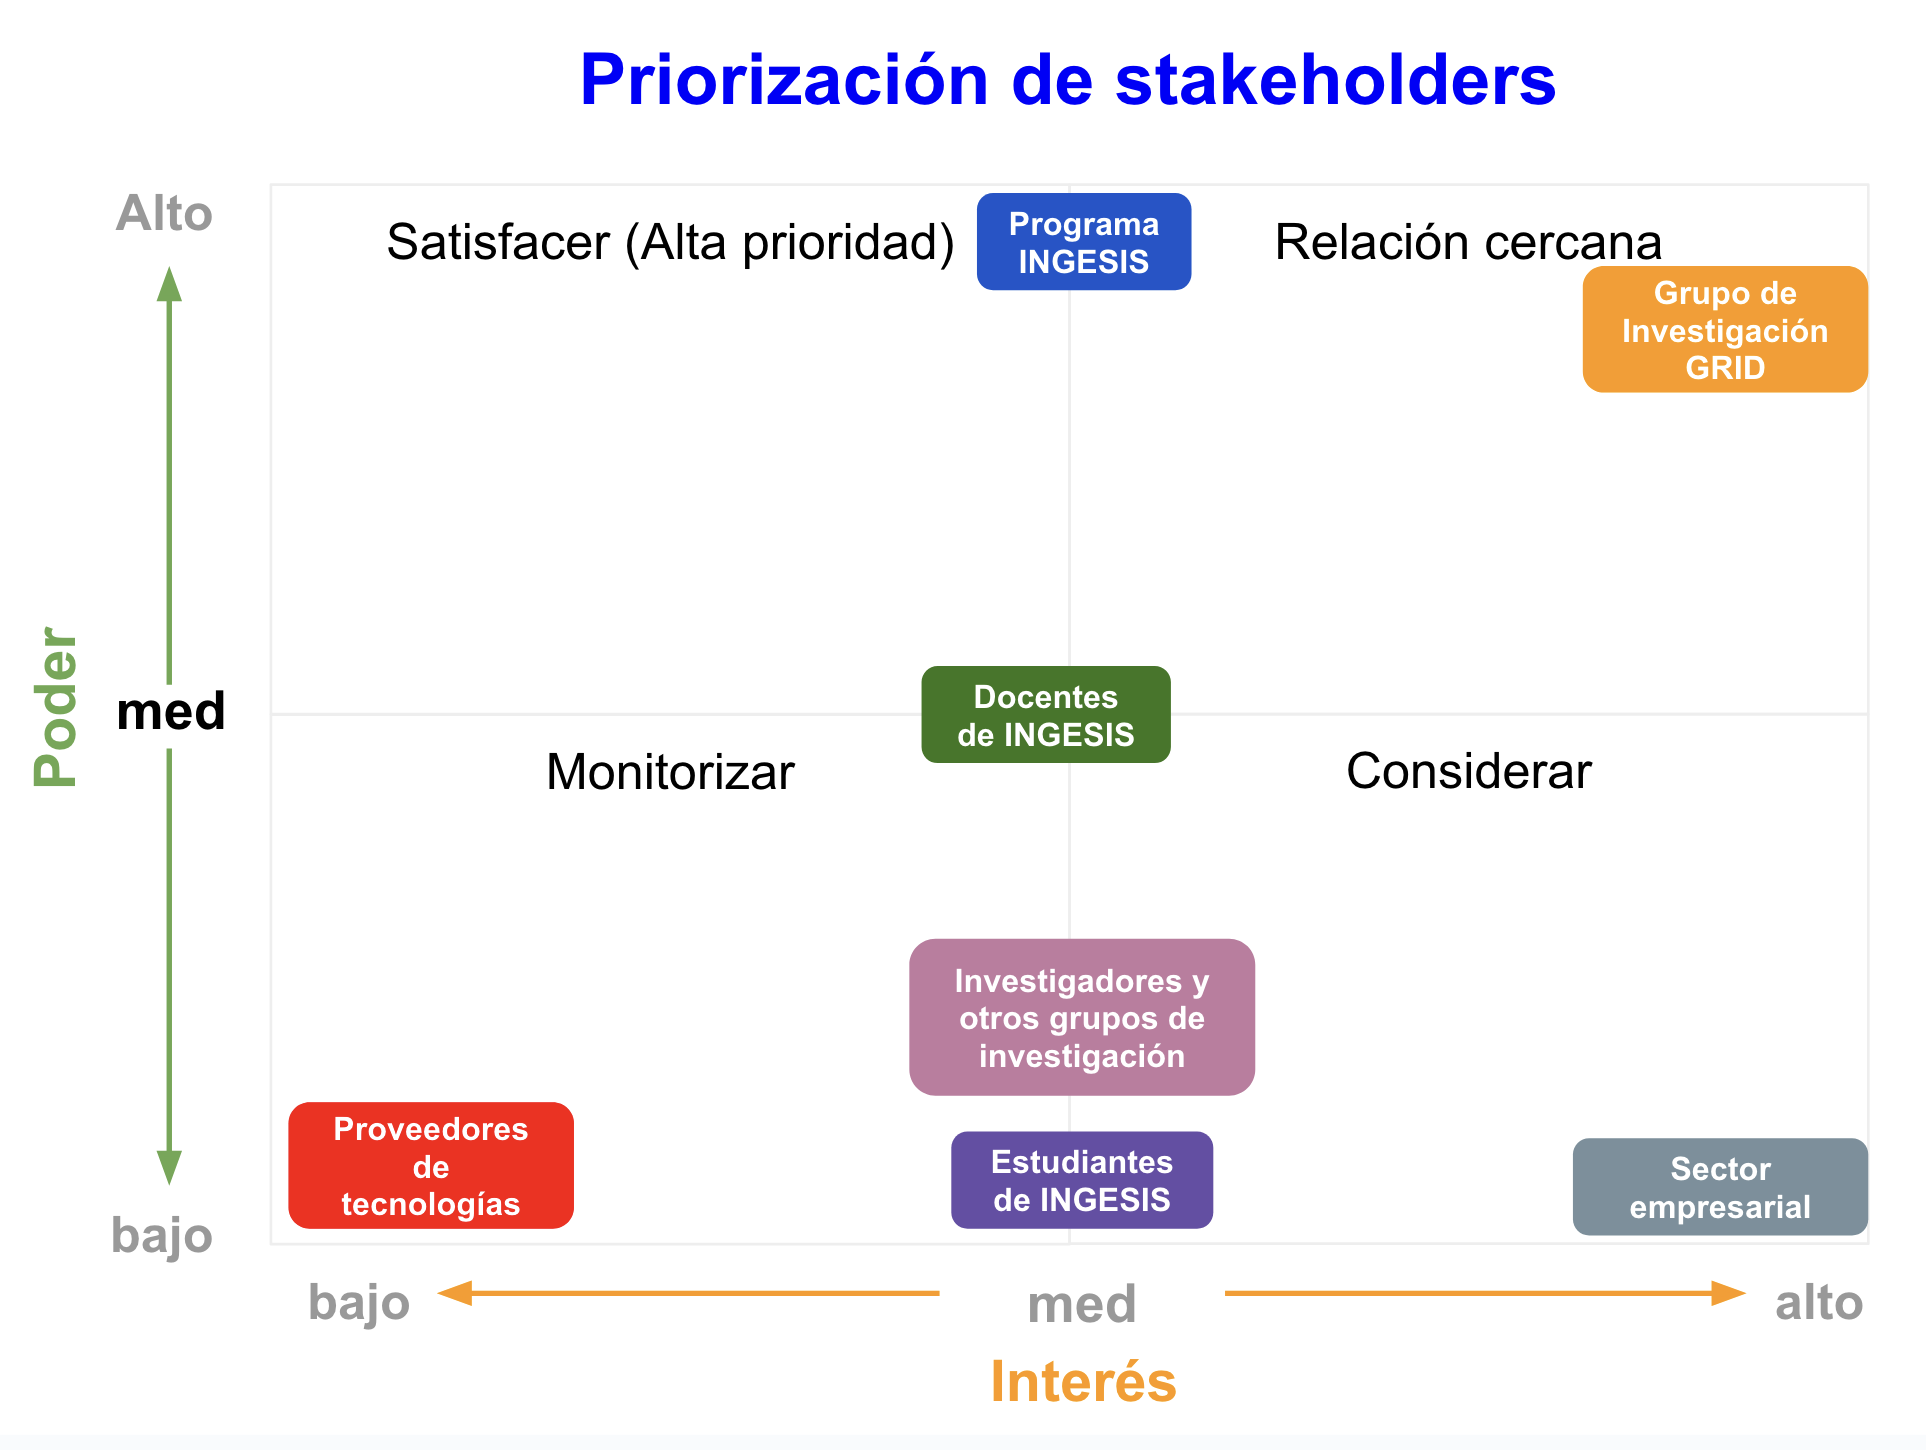
\includegraphics[width=\textwidth] {tablas-images/cp1/priorizacionStakeholders.png}
    \caption{Priorización de stakeholders del proyecto}\label{fig:tabla-priorizacion-stakeholders}
\end{figure}

\section{Integrantes y áreas de trabajo del GRID}
El \GRID está conformado por un equipo multidisciplinario de investigadores y profesionales que, desde sus diferentes áreas de experticia, contribuyen al avance en campos como computación de alto rendimiento, \textit{big data}, inteligencia artificial, redes y desarrollo de software. A continuación, se listan sus integrantes junto con las principales líneas de investigación y trabajo:  

\begin{itemize}
  \item \href{https://scienti.minciencias.gov.co/cvlac/visualizador/generarCurriculoCv.do?cod_rh=0000210897}{\underline{{\textbf{Christian Andrés Candela Uribe}}}}: Microservicios, desarrollo de software, minería de datos, infraestructura TI.\@
  \item \href{https://scienti.minciencias.gov.co/cvlac/visualizador/generarCurriculoCv.do?cod_rh=0001383939}{\underline{{\textbf{Luis Eduardo Sepúlveda Rodríguez}}}}: Infraestructura de TI, HPC, computación paralela.
  \item \href{https://scienti.minciencias.gov.co/cvlac/visualizador/generarCurriculoCv.do?cod_rh=0001638854}{\underline{{\textbf{Carlos Andrés Flórez Villarraga}}}}: Programación y algoritmia, inteligencia artificial.
  \item \href{https://scienti.minciencias.gov.co/cvlac/visualizador/generarCurriculoCv.do?cod_rh=0001343801}{\underline{{\textbf{Carlos Eduardo Gómez Montoya}}}}: Redes, ingeniería de software, cloud computing.
  \item \href{https://scienti.minciencias.gov.co/cvlac/visualizador/generarCurriculoCv.do?cod_rh=0001398775}{\underline{{\textbf{Sergio Augusto Cardona Torres}}}}: Big data y análisis de datos, ingeniería de software, sistemas adaptativos, informática educativa.
  \item \href{https://scienti.minciencias.gov.co/cvlac/visualizador/generarCurriculoCv.do?cod_rh=0000193550}{\underline{{\textbf{Sonia Jaramillo Valbuena}}}}: Big data, electroquímica, inteligencia artificial.
  \item \href{https://scienti.minciencias.gov.co/cvlac/visualizador/generarCurriculoCv.do?cod_rh=0000283495}{\underline{{\textbf{Julián Esteban Gutiérrez Posada}}}}: Microservicios, desarrollo de software, minería de datos, infraestructura TI, HPC, computación paralela, redes, ingeniería de software.
\end{itemize}

La diversidad de líneas de trabajo de los integrantes fortalece la capacidad del grupo para abordar proyectos de carácter transversal y multidisciplinario, lo cual resulta particularmente relevante para el diseño e implementación de soluciones arquitectónicas soportadas en tecnologías de virtualización.

\section{Misión del GRID}
La misión del GRID es heredada de la Universidad del Quindío. A continuación se presenta la misión del GRID:\@

\begin{quote}
\textit{La Universidad del Quindío contribuye a la transformación de la sociedad, mediante la formación integral desde el ser, el saber y el hacer, de líderes reflexivos y gestores del cambio; con estándares de calidad, a través de una oferta de formación en diferentes metodologías, que responda a una sociedad basada en el conocimiento; una investigación pertinente, que aporte a la solución de las problemáticas del desarrollo e integrada con la extensión y proyección social; educando en tiempos del posconflicto y de la consolidación de la paz, apoyada en una gestión creativa y con estándares de calidad.}
\end{quote}

A partir de esta misión, se identifican los siguientes pilares fundamentales:

\begin{itemize}
    \item \textbf{Docencia:} La Universidad del Quindío contribuye a la transformación de la sociedad, mediante la formación integral desde el ser, el saber y el hacer, de líderes reflexivos y gestores del cambio; con estándares de calidad, a través de una oferta de formación en diferentes metodologías, que responda a una sociedad basada en el conocimiento.

    \item \textbf{Investigación:} Una investigación pertinente, que aporte a la solución de las problemáticas del desarrollo e integrada con la extensión y proyección social.

    \item \textbf{Extensión y Desarrollo Social:} Apoyada en una gestión creativa y con estándares de calidad.

    \item \textbf{Responsabilidad Social:} Educando en tiempos del posconflicto y de la consolidación de la paz.
\end{itemize}

\section{Visión del GRID}
La misión de la Universidad del Quindío se complementa con su visión institucional, la cual también es adoptada por el \GRID. A continuación se presenta la visión del \GRID:\@

\begin{quote}
\textit{En el año 2025, la Universidad del Quindío estará consolidada como una institución \textit{Pertinente --- Creativa --- Integradora}, acreditada de alta calidad, con reconocimiento nacional e internacional en sus procesos de formación a través de diferentes metodologías, de investigación, extensión, proyección y responsabilidad social.}
\end{quote}

A partir de esta visión, se destacan los siguientes enfoques estratégicos:

\begin{itemize}
    \item \textbf{Gestión:} La Universidad del Quindío estará consolidada como una institución \textit{Pertinente --- Creativa --- Integradora}.

    \item \textbf{Docencia:} Acreditada de alta calidad en sus procesos de formación a través de diferentes metodologías.

    \item \textbf{Investigación:} Consolidada como pertinente y de alta calidad en sus procesos de investigación.

    \item \textbf{Extensión y Desarrollo Social:} Procesos creativos e integradores en proyección social.

    \item \textbf{Responsabilidad Social:} Reconocimientos en sus procesos de responsabilidad social.
\end{itemize}

\section{Impacto del proyecto en el GRID}

El proyecto tiene como objetivo apoyar los procesos de docencia, investigación
y extensión mediante la especificación de una arquitectura de tecnologías de 
virtualización basada en contenedores (\VBC). 

Este trabajo se enfoca en la identificación de una tecnología de contenerización que 
\textbf{agregue valor a los procesos del \GRID}, beneficiando a docentes, estudiantes
y cualquier parte interesada que participe en los proyectos y actividades desarrolladas 
por este grupo de investigación.

\section{Caracterización de la infraestructura tecnológica del GRID}
En el siguiente formato se van a especificar las características técnicas de la infraestructura tecnológica del GRID disponible para temas de virtualización.\ \href{https://docs.google.com/spreadsheets/d/14NBv72ucVTrLqGIldYdIsjdBGt3QlgwcblcVRis-DaQ/edit?usp=sharing}{Macro de la ficha técnica}
% Archivo de caracterización de infraestructura corregido

% Torre HP 1
\begin{table}[H]
\centering
\scriptsize % Tamaño de fuente más pequeño
\setlength{\tabcolsep}{2pt} % Menor espacio entre columnas
\renewcommand{\arraystretch}{1.0} % Espaciado más ajustado
\caption{Ficha técnica --- Torre 1}\label{tab:torre-hp-1}
\begin{tabular}{|p{0.5\textwidth}|p{0.2\textwidth}|} % Columnas más estrechas
\hline
\multicolumn{2}{|l|}{\textbf{DESCRIPCIÓN FÍSICA:} Servidor tipo torre} \\ \hline
\textbf{TIPO DE RECURSO:} Torre &
\multirow{5}{*}{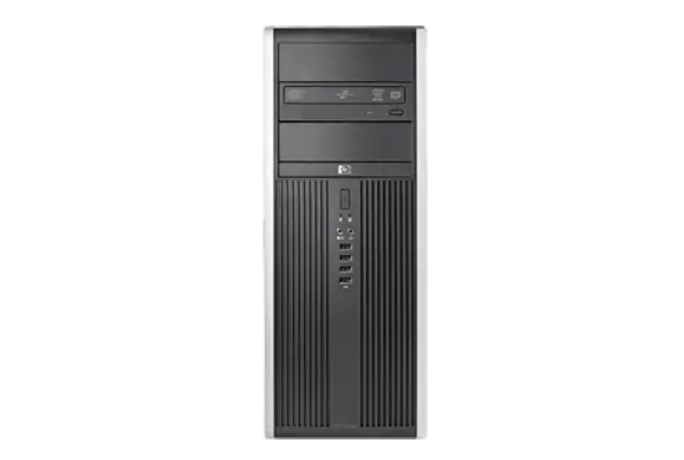
\includegraphics[width=0.18\textwidth,keepaspectratio]{tablas-images/cp1/torres/torre-1.png}} \\ \cline{1-1}
\textbf{MODELO:} Desconocido & \\ \cline{1-1}
\textbf{MARCA:} HP & \\ \cline{1-1}
\textbf{CÓDIGO DE INVENTARIO:} 7 24390 49867 3 & \\ \cline{1-1}
\textbf{NÚMERO EN CPD:} 14 & \\ \hline
\multicolumn{2}{|l|}{\textbf{ESPECIFICACIONES TÉCNICAS}} \\ \hline
\multicolumn{2}{|p{0.7\textwidth}|}{ % Ancho ajustado
- 8 USB (4 frontal, 4 trasera)
- Audio y micrófono
- HDMI
- Lector DVD
- 3 Ethernet
- DisplayPort
- PS/2 (Teclado/Ratón)
} \\ \hline
\multicolumn{2}{|l|}{\textbf{PROPÓSITO:} Hipervisor XCP-ng} \\ \hline
\multicolumn{2}{|l|}{\textbf{OPORTUNIDAD DE USO:} Proyectos del \GRID} \\ \hline
\multicolumn{2}{|p{0.7\textwidth}|}{\textbf{OBSERVACIONES:} Sin modelo. Equipo adaptado para virtualización.} \\ \hline
\end{tabular}
\end{table}

% Torre 2
\begin{table}[H]
\centering
\scriptsize
\setlength{\tabcolsep}{2pt}
\renewcommand{\arraystretch}{1.0}
\caption{Ficha técnica --- Torre 2}\label{tab:torre-2}
\begin{tabular}{|p{0.5\textwidth}|p{0.2\textwidth}|}
\hline
\multicolumn{2}{|l|}{\textbf{DESCRIPCIÓN FÍSICA:} Servidor tipo torre} \\ \hline
\textbf{TIPO DE RECURSO:} Torre & 
\multirow{5}{*}{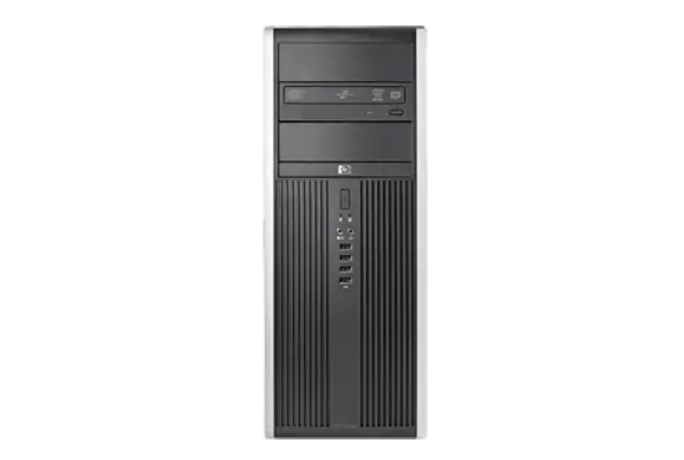
\includegraphics[width=0.18\textwidth,keepaspectratio]{tablas-images/cp1/torres/torre-1.png}} \\ \cline{1-1}
\textbf{MODELO:} Desconocido & \\ \cline{1-1}
\textbf{MARCA:} HP & \\ \cline{1-1}
\textbf{CÓDIGO DE INVENTARIO:} 7 24390 49861 1 & \\ \cline{1-1}
\textbf{NÚMERO EN CPD:} 12 & \\ \hline
\multicolumn{2}{|l|}{\textbf{ESPECIFICACIONES TÉCNICAS}} \\ \hline
\multicolumn{2}{|p{0.7\textwidth}|}{
- 8 USB (4 frontal, 4 trasera)
- Audio y micrófono
- HDMI
- Lector DVD
- 3 Ethernet
- DisplayPort
- PS/2 (Teclado/Ratón)
} \\ \hline
\multicolumn{2}{|l|}{\textbf{PROPÓSITO:} Hipervisor XCP-ng} \\ \hline
\multicolumn{2}{|l|}{\textbf{OPORTUNIDAD DE USO:} Proyectos del \GRID} \\ \hline
\multicolumn{2}{|p{0.7\textwidth}|}{\textbf{OBSERVACIONES:} Sin modelo. Equipo adaptado para virtualización.} \\ \hline
\end{tabular}
\end{table}

% Torre 3
\begin{table}[H]
\centering
\scriptsize
\setlength{\tabcolsep}{2pt}
\renewcommand{\arraystretch}{1.0}
\caption{Ficha técnica -- Torre 3}
\label{tab:torre-3}
\begin{tabular}{|p{0.5\textwidth}|p{0.2\textwidth}|}
\hline
\multicolumn{2}{|l|}{\textbf{DESCRIPCIÓN FÍSICA:} Servidor tipo torre} \\ \hline
\textbf{TIPO DE RECURSO:} Torre & 
\multirow{5}{*}{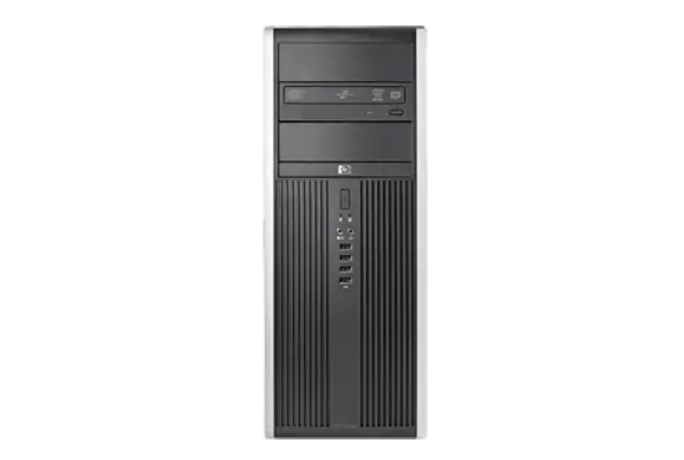
\includegraphics[width=0.18\textwidth,keepaspectratio]{tablas-images/cp1/torres/torre-1.png}} \\ \cline{1-1}
\textbf{MODELO:} Desconocido & \\ \cline{1-1}
\textbf{MARCA:} HP & \\ \cline{1-1}
\textbf{CÓDIGO DE INVENTARIO:} 7 24390 49969 4 & \\ \cline{1-1}
\textbf{NÚMERO EN CPD:} 13 & \\ \hline
\multicolumn{2}{|l|}{\textbf{ESPECIFICACIONES TÉCNICAS}} \\ \hline
\multicolumn{2}{|p{0.7\textwidth}|}{
- 8 USB (4 frontal, 4 trasera)
- Audio y micrófono
- HDMI
- Lector DVD
- 3 Ethernet
- DisplayPort
- PS/2 (Teclado/Ratón)
} \\ \hline
\multicolumn{2}{|l|}{\textbf{PROPÓSITO:} Hipervisor XCP-ng} \\ \hline
\multicolumn{2}{|l|}{\textbf{OPORTUNIDAD DE USO:} Proyectos del \GRID} \\ \hline
\multicolumn{2}{|p{0.7\textwidth}|}{\textbf{OBSERVACIONES:} Sin modelo. Equipo adaptado para virtualización.} \\ \hline
\end{tabular}
\end{table}

% Torre 4
\begin{table}[H]
\centering
\scriptsize
\setlength{\tabcolsep}{2pt}
\renewcommand{\arraystretch}{1.0}
\caption{Ficha técnica --- Torre 4}\label{tab:torre-4}
\begin{tabular}{|p{0.5\textwidth}|p{0.2\textwidth}|}
\hline
\multicolumn{2}{|l|}{\textbf{DESCRIPCIÓN FÍSICA:} Servidor tipo torre} \\ \hline
\textbf{TIPO DE RECURSO:} Torre & 
\multirow{5}{*}{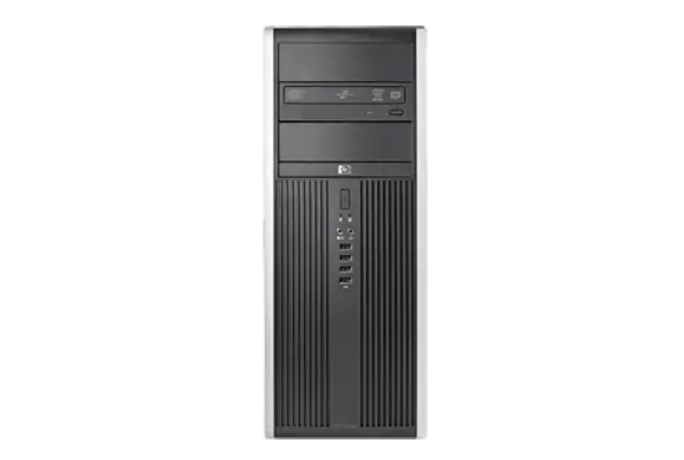
\includegraphics[width=0.18\textwidth,keepaspectratio]{tablas-images/cp1/torres/torre-1.png}} \\ \cline{1-1}
\textbf{MODELO:} Desconocido & \\ \cline{1-1}
\textbf{MARCA:} HP & \\ \cline{1-1}
\textbf{CÓDIGO DE INVENTARIO:} 7 24390 49879 4 & \\ \cline{1-1}
\textbf{NÚMERO EN CPD:} 14 & \\ \hline
\multicolumn{2}{|l|}{\textbf{ESPECIFICACIONES TÉCNICAS}} \\ \hline
\multicolumn{2}{|p{0.7\textwidth}|}{
- 8 USB (4 frontal, 4 trasera)
- Audio y micrófono
- HDMI
- Lector DVD
- 3 Ethernet
- DisplayPort
- PS/2 (Teclado/Ratón)
} \\ \hline
\multicolumn{2}{|l|}{\textbf{PROPÓSITO:} Hipervisor XCP-ng} \\ \hline
\multicolumn{2}{|l|}{\textbf{OPORTUNIDAD DE USO:} Proyectos del \GRID} \\ \hline
\multicolumn{2}{|p{0.7\textwidth}|}{\textbf{OBSERVACIONES:} Sin modelo. Equipo adaptado para virtualización.} \\ \hline
\end{tabular}
\end{table}

% Torre 5
\begin{table}[H]
\centering
\scriptsize
\setlength{\tabcolsep}{2pt}
\renewcommand{\arraystretch}{1.0}
\caption{Ficha técnica --- Torre 5}
\label{tab:torre-5}
\begin{tabular}{|p{0.5\textwidth}|p{0.2\textwidth}|}
\hline
\multicolumn{2}{|l|}{\textbf{DESCRIPCIÓN FÍSICA:} Servidor tipo torre} \\ \hline
\textbf{TIPO DE RECURSO:} Torre & 
\multirow{5}{*}{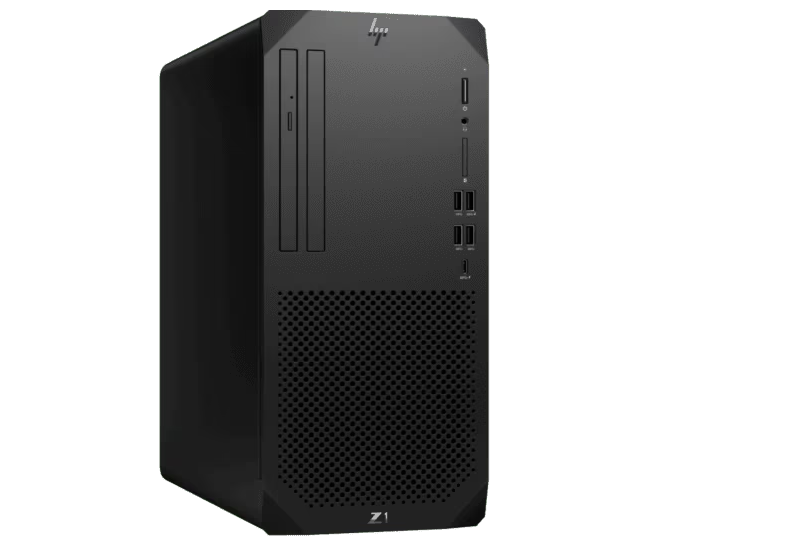
\includegraphics[width=0.18\textwidth,keepaspectratio]{tablas-images/cp1/torres/torre-2.png}} \\ \cline{1-1}
\textbf{MODELO:} G9 & \\ \cline{1-1}
\textbf{MARCA:} HP & \\ \cline{1-1}
\textbf{CÓDIGO DE INVENTARIO:} 72992 & \\ \cline{1-1}
\textbf{NÚMERO EN CPD:} 22 & \\ \hline
\multicolumn{2}{|l|}{\textbf{ESPECIFICACIONES TÉCNICAS}} \\ \hline
\multicolumn{2}{|p{0.7\textwidth}|}{
- 9 USB (4 frontal, 5 trasera)
- Audio y micrófono
- HDMI
- Lector DVD
- 1 Ethernet
- 2 DisplayPort
- Procesador Intel vPro i9
} \\ \hline
\multicolumn{2}{|l|}{\textbf{PROPÓSITO:} Hipervisor XCP-ng} \\ \hline
\multicolumn{2}{|l|}{\textbf{OPORTUNIDAD DE USO:} Proyectos del \GRID} \\ \hline
\multicolumn{2}{|p{0.7\textwidth}|}{\textbf{OBSERVACIONES:} Equipo adaptado para virtualización.} \\ \hline
\end{tabular}
\end{table}

% Torre 6
\begin{table}[H]
\centering
\scriptsize
\setlength{\tabcolsep}{2pt}
\renewcommand{\arraystretch}{1.0}
\caption{Ficha técnica --- Torre 6}
\label{tab:torre-6}
\begin{tabular}{|p{0.5\textwidth}|p{0.2\textwidth}|}
\hline
\multicolumn{2}{|l|}{\textbf{DESCRIPCIÓN FÍSICA:} Servidor tipo torre} \\ \hline
\textbf{TIPO DE RECURSO:} Torre & 
\multirow{5}{*}{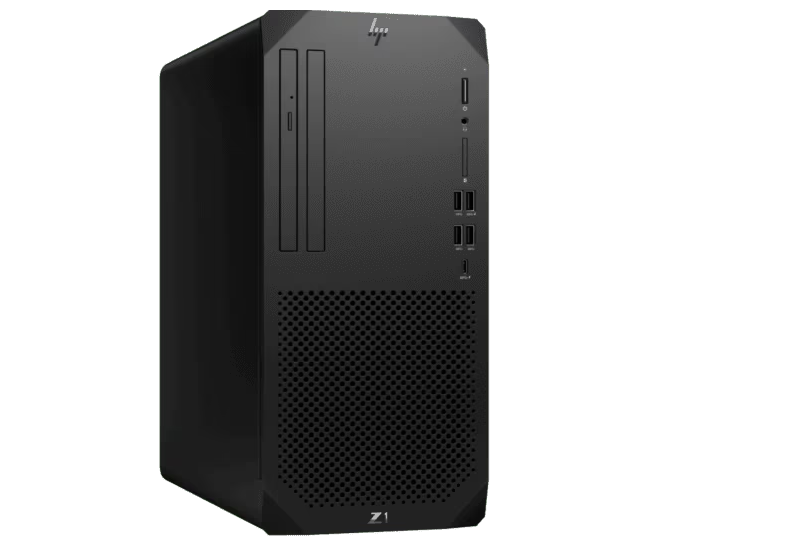
\includegraphics[width=0.18\textwidth,keepaspectratio]{tablas-images/cp1/torres/torre-2.png}} \\ \cline{1-1}
\textbf{MODELO:} G9 & \\ \cline{1-1}
\textbf{MARCA:} HP & \\ \cline{1-1}
\textbf{CÓDIGO DE INVENTARIO:} 72976 & \\ \cline{1-1}
\textbf{NÚMERO EN CPD:} 21 & \\ \hline
\multicolumn{2}{|l|}{\textbf{ESPECIFICACIONES TÉCNICAS}} \\ \hline
\multicolumn{2}{|p{0.7\textwidth}|}{
- 9 USB (4 frontal, 5 trasera)
- Audio y micrófono
- HDMI
- Lector DVD
- 1 Ethernet
- 2 DisplayPort
- Procesador Intel vPro i9
} \\ \hline
\multicolumn{2}{|l|}{\textbf{PROPÓSITO:} Hipervisor XCP-ng} \\ \hline
\multicolumn{2}{|l|}{\textbf{OPORTUNIDAD DE USO:} Proyectos del \GRID} \\ \hline
\multicolumn{2}{|p{0.7\textwidth}|}{\textbf{OBSERVACIONES:} Equipo adaptado para virtualización.} \\ \hline
\end{tabular}
\end{table}

% Torre 7
\begin{table}[H]
\centering
\scriptsize
\setlength{\tabcolsep}{2pt}
\renewcommand{\arraystretch}{1.0}
\caption{Ficha técnica --- Torre 7}
\label{tab:torre-7}
\begin{tabular}{|p{0.5\textwidth}|p{0.2\textwidth}|}
\hline
\multicolumn{2}{|l|}{\textbf{DESCRIPCIÓN FÍSICA:} Servidor tipo torre} \\ \hline
\textbf{TIPO DE RECURSO:} Torre & 
\multirow{5}{*}{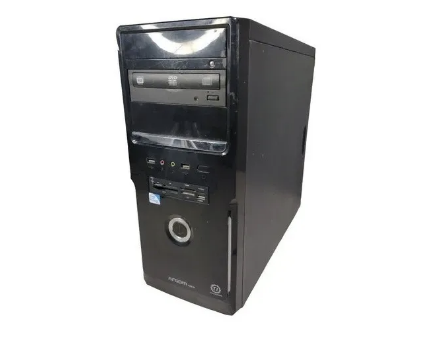
\includegraphics[width=0.18\textwidth,keepaspectratio]{tablas-images/cp1/torres/ATX.png}} \\ \cline{1-1}
\textbf{MODELO:} Argom tech & \\ \cline{1-1}
\textbf{MARCA:} Argom tech & \\ \cline{1-1}
\textbf{CÓDIGO DE INVENTARIO:} Sin código & \\ \cline{1-1}
\textbf{NÚMERO EN CPD:} 11 & \\ \hline
\multicolumn{2}{|l|}{\textbf{ESPECIFICACIONES TÉCNICAS}} \\ \hline
\multicolumn{2}{|p{0.7\textwidth}|}{
- Procesador: Intel Pentium 62030 3.00GHz
- Arquitectura: X64
- RAM: 16GB
- Disco: 1024GB
- Unidad CD/DVD: Sí
- Tarjeta video: Integrada
- Tarjeta sonido: Integrada
} \\ \hline
\multicolumn{2}{|l|}{\textbf{PROPÓSITO:} Hipervisor XCP-ng} \\ \hline
\multicolumn{2}{|l|}{\textbf{OPORTUNIDAD DE USO:} Proyectos del \GRID} \\ \hline
\multicolumn{2}{|p{0.7\textwidth}|}{\textbf{OBSERVACIONES:} Equipo adaptado para virtualización.} \\ \hline
\end{tabular}
\end{table}

% Rack 1
\begin{table}[H]
\centering
\scriptsize
\setlength{\tabcolsep}{2pt}
\renewcommand{\arraystretch}{1.0}
\caption{Ficha técnica --- Rack 1}
\label{tab:rack-1}
\begin{tabular}{|p{0.5\textwidth}|p{0.2\textwidth}|}
\hline
\multicolumn{2}{|l|}{\textbf{DESCRIPCIÓN FÍSICA:} Servidor tipo rack} \\ \hline
\textbf{TIPO DE RECURSO:} Servidor & 
\multirow{5}{*}{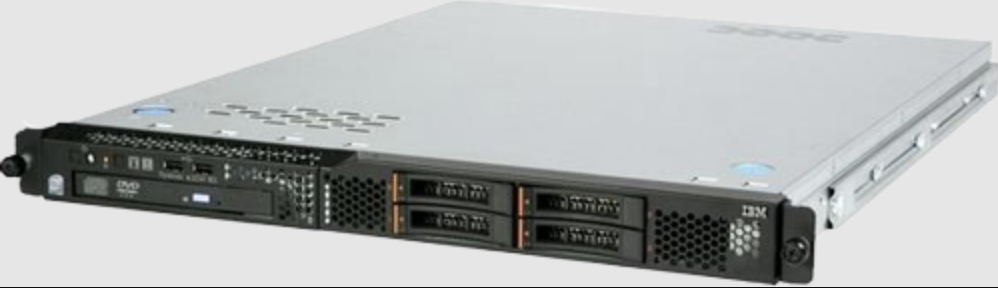
\includegraphics[width=0.18\textwidth,keepaspectratio]{tablas-images/cp1/racks/rack-1.png}} \\ \cline{1-1}
\textbf{MODELO:} System x3250 M4 & \\ \cline{1-1}
\textbf{MARCA:} IBM & \\ \cline{1-1}
\textbf{CÓDIGO DE INVENTARIO:} 7 24390 50981 & \\ \cline{1-1}
\textbf{NUMERO EN CPD:} 55 & \\ \hline
\multicolumn{2}{|l|}{\textbf{ESPECIFICACIONES TÉCNICAS}} \\ \hline
\multicolumn{2}{|p{0.7\textwidth}|}{
- Procesador Intel Xeon E3-1220v2
- Controlador SATA integrado
- 2 ranuras PCI Express
- 4 SAS/SATA intercambio en caliente
- Fuente redundante 460W
- Gestión del sistema
- 4 puertos USB (2 frontal, 2 trasero)
- Lector DVD
} \\ \hline
\multicolumn{2}{|l|}{\textbf{PROPÓSITO:} Prestación de servicios de cómputo} \\ \hline
\multicolumn{2}{|p{0.7\textwidth}|}{\textbf{IMPACTO:} 
- Servicios a estudiantes
- Máquinas virtuales para prácticas} \\ \hline
\multicolumn{2}{|p{0.7\textwidth}|}{\textbf{OBSERVACIONES:} Ninguna} \\ \hline
\end{tabular}
\end{table}

% Rack 2
\begin{table}[H]
\centering
\scriptsize
\setlength{\tabcolsep}{2pt}
\renewcommand{\arraystretch}{1.0}
\caption{Ficha técnica --- Rack 2}
\label{tab:rack-2}
\begin{tabular}{|p{0.5\textwidth}|p{0.2\textwidth}|}
\hline
\multicolumn{2}{|l|}{\textbf{DESCRIPCIÓN FÍSICA:} Servidor tipo rack} \\ \hline
\textbf{TIPO DE RECURSO:} Servidor & 
\multirow{5}{*}{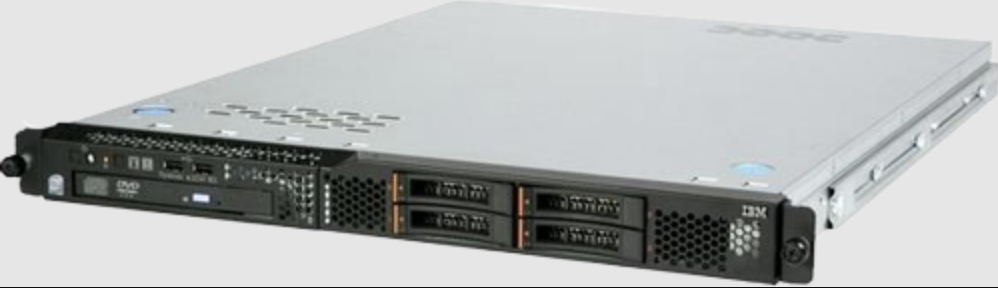
\includegraphics[width=0.18\textwidth,keepaspectratio]{tablas-images/cp1/racks/rack-1.png}} \\ \cline{1-1}
\textbf{MODELO:} System x3250 M4 & \\ \cline{1-1}
\textbf{MARCA:} IBM & \\ \cline{1-1}
\textbf{CÓDIGO DE INVENTARIO:} 7 24390 50980 & \\ \cline{1-1}
\textbf{NUMERO EN CPD:} 54 & \\ \hline
\multicolumn{2}{|l|}{\textbf{ESPECIFICACIONES TÉCNICAS}} \\ \hline
\multicolumn{2}{|p{0.7\textwidth}|}{
- Procesador Intel Xeon E3-1220v2
- Controlador SATA integrado
- 2 ranuras PCI Express
- 4 SAS/SATA intercambio en caliente
- Fuente redundante 460W
- Gestión del sistema
- 4 puertos USB (2 frontal, 2 trasero)
- Lector DVD
} \\ \hline
\multicolumn{2}{|l|}{\textbf{PROPÓSITO:} Prestación de servicios de cómputo} \\ \hline
\multicolumn{2}{|p{0.7\textwidth}|}{\textbf{IMPACTO:} 
- Servicios a estudiantes
- Máquinas virtuales para prácticas} \\ \hline
\multicolumn{2}{|p{0.7\textwidth}|}{\textbf{OBSERVACIONES:} Ninguna} \\ \hline
\end{tabular}
\end{table}

% Rack 3
\begin{table}[H]
\centering
\scriptsize
\setlength{\tabcolsep}{2pt}
\renewcommand{\arraystretch}{1.0}
\caption{Ficha técnica --- Rack 3}
\label{tab:rack-3}
\begin{tabular}{|p{0.5\textwidth}|p{0.2\textwidth}|}
\hline
\multicolumn{2}{|l|}{\textbf{DESCRIPCIÓN FÍSICA:} Servidor tipo rack} \\ \hline
\textbf{TIPO DE RECURSO:} Servidor & 
\multirow{5}{*}{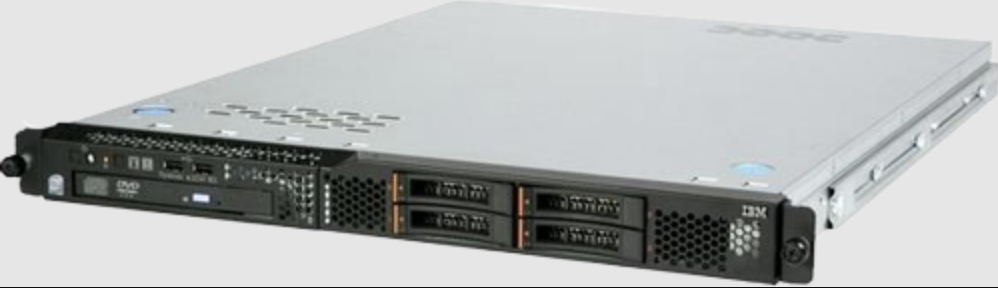
\includegraphics[width=0.18\textwidth,keepaspectratio]{tablas-images/cp1/racks/rack-1.png}} \\ \cline{1-1}
\textbf{MODELO:} System x3250 M4 & \\ \cline{1-1}
\textbf{MARCA:} IBM & \\ \cline{1-1}
\textbf{CÓDIGO DE INVENTARIO:} 7 24390 50980 & \\ \cline{1-1}
\textbf{NUMERO EN CPD:} 53 & \\ \hline
\multicolumn{2}{|l|}{\textbf{ESPECIFICACIONES TÉCNICAS}} \\ \hline
\multicolumn{2}{|p{0.7\textwidth}|}{
- Procesador Intel Xeon E3-1220v2
- Controlador SATA integrado
- 2 ranuras PCI Express
- 4 SAS/SATA intercambio en caliente
- Fuente redundante 460W
- Gestión del sistema
- 4 puertos USB (2 frontal, 2 trasero)
- Lector DVD
} \\ \hline
\multicolumn{2}{|l|}{\textbf{PROPÓSITO:} Prestación de servicios de cómputo} \\ \hline
\multicolumn{2}{|p{0.7\textwidth}|}{\textbf{IMPACTO:} 
- Servicios a estudiantes
- Máquinas virtuales para prácticas} \\ \hline
\multicolumn{2}{|p{0.7\textwidth}|}{\textbf{OBSERVACIONES:} Ninguna} \\ \hline
\end{tabular}
\end{table}

% Rack 4
\begin{table}[H]
\centering
\scriptsize
\setlength{\tabcolsep}{2pt}
\renewcommand{\arraystretch}{1.0}
\caption{Ficha técnica --- Rack 4}
\label{tab:rack-4}
\begin{tabular}{|p{0.5\textwidth}|p{0.2\textwidth}|}
\hline
\multicolumn{2}{|l|}{\textbf{DESCRIPCIÓN FÍSICA:} Servidor tipo rack} \\ \hline
\textbf{TIPO DE RECURSO:} Servidor & 
\multirow{5}{*}{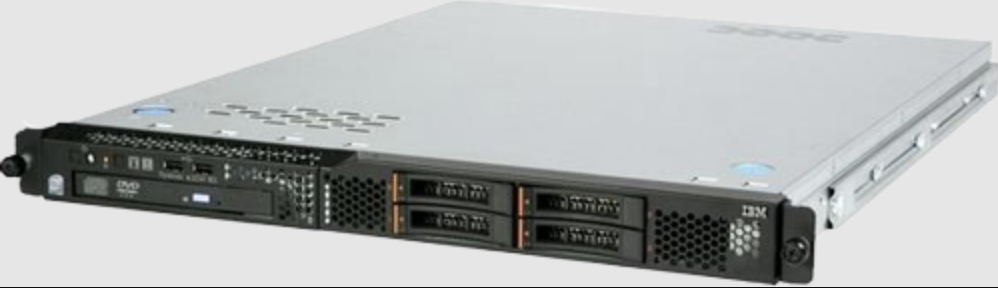
\includegraphics[width=0.18\textwidth,keepaspectratio]{tablas-images/cp1/racks/rack-1.png}} \\ \cline{1-1}
\textbf{MODELO:} System x3250 M4 & \\ \cline{1-1}
\textbf{MARCA:} IBM & \\ \cline{1-1}
\textbf{CÓDIGO DE INVENTARIO:} 7 24390 48735 & \\ \cline{1-1}
\textbf{NUMERO EN CPD:} 52 & \\ \hline
\multicolumn{2}{|l|}{\textbf{ESPECIFICACIONES TÉCNICAS}} \\ \hline
\multicolumn{2}{|p{0.7\textwidth}|}{
- Procesador Intel Xeon E3-1220v2
- Controlador SATA integrado
- 2 ranuras PCI Express
- 4 SAS/SATA intercambio en caliente
- Fuente redundante 460W
- Gestión del sistema
- 4 puertos USB (2 frontal, 2 trasero)
- Lector DVD
} \\ \hline
\multicolumn{2}{|l|}{\textbf{PROPÓSITO:} Prestación de servicios de cómputo} \\ \hline
\multicolumn{2}{|p{0.7\textwidth}|}{\textbf{IMPACTO:} 
- Servicios a estudiantes
- Máquinas virtuales para prácticas} \\ \hline
\multicolumn{2}{|p{0.7\textwidth}|}{\textbf{OBSERVACIONES:} Ninguna} \\ \hline
\end{tabular}
\end{table}

% Rack 5
\begin{table}[H]
\centering
\scriptsize
\setlength{\tabcolsep}{2pt}
\renewcommand{\arraystretch}{1.0}
\caption{Ficha técnica --- Rack 5}\label{tab:rack-5}
\begin{tabular}{|p{0.5\textwidth}|p{0.2\textwidth}|}
\hline
\multicolumn{2}{|l|}{\textbf{DESCRIPCIÓN FÍSICA:} Servidor tipo rack} \\ \hline
\textbf{TIPO DE RECURSO:} Servidor & 
\multirow{5}{*}{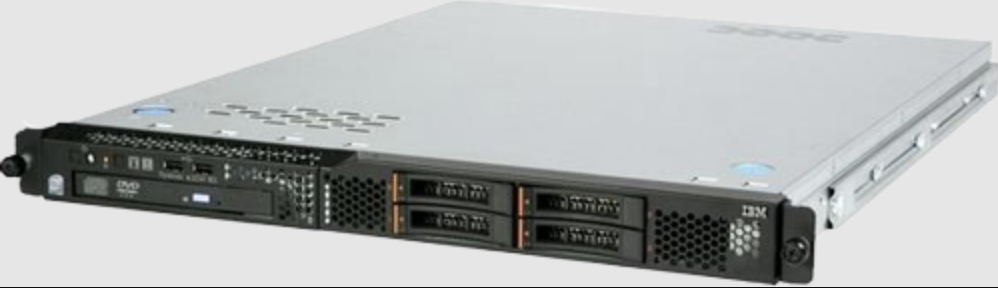
\includegraphics[width=0.18\textwidth,keepaspectratio]{tablas-images/cp1/racks/rack-1.png}} \\ \cline{1-1}
\textbf{MODELO:} System x3250 M4 & \\ \cline{1-1}
\textbf{MARCA:} IBM & \\ \cline{1-1}
\textbf{CÓDIGO DE INVENTARIO:} 51474 & \\ \cline{1-1}
\textbf{NUMERO EN CPD:} 52 & \\ \hline
\multicolumn{2}{|l|}{\textbf{ESPECIFICACIONES TÉCNICAS}} \\ \hline
\multicolumn{2}{|p{0.7\textwidth}|}{
- Procesador Intel Xeon E3-1220v2
- Controlador SATA integrado
- 2 ranuras PCI Express
- 4 SAS/SATA intercambio en caliente
- Fuente redundante 460W
- Gestión del sistema
- 4 puertos USB (2 frontal, 2 trasero)
- Lector DVD
} \\ \hline
\multicolumn{2}{|l|}{\textbf{PROPÓSITO:} Prestación de servicios de cómputo} \\ \hline
\multicolumn{2}{|p{0.7\textwidth}|}{\textbf{IMPACTO:} 
- Servicios a estudiantes
- Máquinas virtuales para prácticas} \\ \hline
\multicolumn{2}{|p{0.7\textwidth}|}{\textbf{OBSERVACIONES:} Ninguna} \\ \hline
\end{tabular}
\end{table}

% NAS 1
\begin{table}[H]
\centering
\scriptsize
\setlength{\tabcolsep}{2pt}
\renewcommand{\arraystretch}{1.0}
\caption{Ficha técnica --- NAS 1}\label{tab:nas-1}
\begin{tabular}{|p{0.5\textwidth}|p{0.2\textwidth}|}
\hline
\multicolumn{2}{|l|}{\textbf{DESCRIPCIÓN FÍSICA:} Sistema de almacenamiento en red} \\ \hline
\textbf{TIPO DE RECURSO:} NAS & 
\multirow{5}{*}{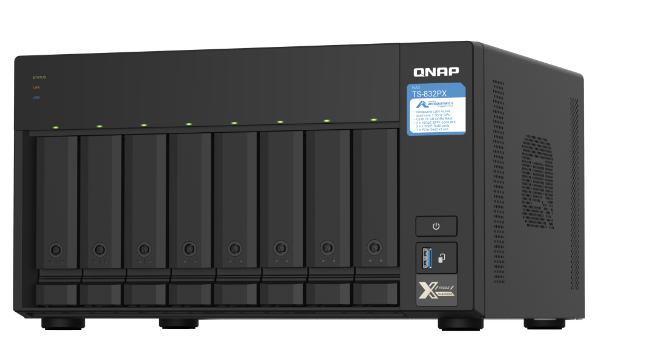
\includegraphics[width=0.18\textwidth,keepaspectratio]{tablas-images/cp1/NAS/nas-1.png}} \\ \cline{1-1}
\textbf{MODELO:} TS-832PX-4G & \\ \cline{1-1}
\textbf{MARCA:} QNAP & \\ \cline{1-1}
\textbf{CÓDIGO DE INVENTARIO:} Por definir & \\ \cline{1-1}
\textbf{FECHA DE ADQUISICIÓN:} & \\ \hline
\multicolumn{2}{|l|}{\textbf{ESPECIFICACIONES TÉCNICAS}} \\ \hline
\multicolumn{2}{|p{0.7\textwidth}|}{
- Procesador: Annapurna Labs Alpine AL-324, 4 núcleos
- RAM: 4 GB DDR4 (exp. a 16 GB)
- Bahías: 8 para discos SATA 3.5"/2.5"
- Puertos Red: 2 x RJ45 2.5GbE, 2 x 10GbE
- Puertos USB: 3 x USB 3.2 Gen 1
- Consumo: 50.8 W (func.), 27 W (reposo)
- Expansión: Ranuras PCIe
} \\ \hline
\multicolumn{2}{|p{0.7\textwidth}|}{\textbf{PROPÓSITO:} Almacenamiento compartido y redundante en red} \\ \hline
\multicolumn{2}{|p{0.7\textwidth}|}{\textbf{IMPACTO:} - Sin NAS: no hay backups ni acceso a archivos} \\ \hline
\multicolumn{2}{|p{0.7\textwidth}|}{\textbf{OBSERVACIONES:} Ninguna} \\ \hline
\end{tabular}
\end{table}

% Firewall 1
\begin{table}[H]
\centering
\scriptsize
\setlength{\tabcolsep}{2pt}
\renewcommand{\arraystretch}{1.0}
\caption{Ficha técnica --- Firewall}\label{tab:firewall-1}
\begin{tabular}{|p{0.5\textwidth}|p{0.2\textwidth}|}
\hline
\multicolumn{2}{|l|}{\textbf{DESCRIPCIÓN FÍSICA:} Sistema de seguridad de red} \\ \hline
\textbf{TIPO DE RECURSO:} Firewall & 
\multirow{5}{*}{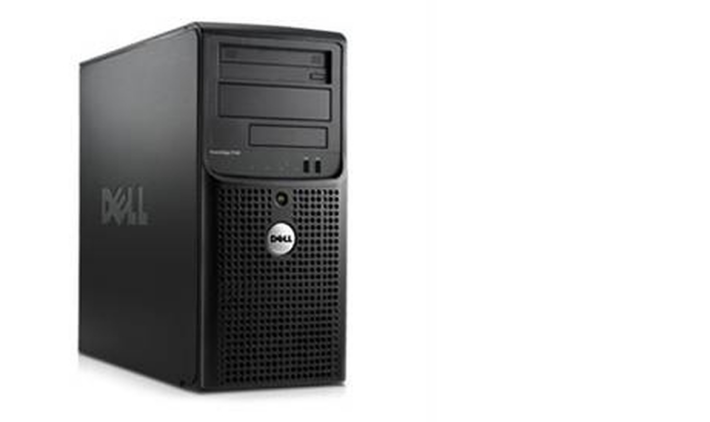
\includegraphics[width=0.18\textwidth,keepaspectratio]{tablas-images/cp1/firewall/firewall.png}} \\ \cline{1-1}
\textbf{MODELO:} PowerEdge T100 & \\ \cline{1-1}
\textbf{MARCA:} DELL & \\ \cline{1-1}
\textbf{CÓDIGO DE INVENTARIO:} 7 24390 46288 9 & \\ \cline{1-1}
\textbf{NÚMERO EN CPF:} No especificado & \\ \hline
\multicolumn{2}{|l|}{\textbf{ESPECIFICACIONES TÉCNICAS}} \\ \hline
\multicolumn{2}{|p{0.7\textwidth}|}{
- Procesador: Intel Xeon E3110 3 GHz
- Memoria: 4 GB DDR2 (2 x 2 GB)
- Almacenamiento: 1 TB HDD 3.5"
- Fuente alimentación: 305 W
- Unidad óptica: DVD-ROM
- Tipo chasis: Torre
- Ethernet
} \\ \hline
\multicolumn{2}{|l|}{\textbf{PROPÓSITO:} Seguridad de la red de servidores} \\ \hline
\multicolumn{2}{|p{0.7\textwidth}|}{\textbf{IMPACTO:} - Protege equipos de usuarios no autorizados} \\ \hline
\multicolumn{2}{|p{0.7\textwidth}|}{\textbf{OBSERVACIONES:} Ninguna} \\ \hline
\end{tabular}
\end{table}

\section{Caracterización de servicios del GRID}
El \GRID\ ofrece una variedad de servicios tecnológicos a la comunidad académica, especialmente a los estudiantes de Ingeniería de Sistemas y Computación. Estos servicios incluyen:

\subsection{Servicios actuales}
Los servicios actuales del GRID se centran en la provisión de infraestructura de \TI\, incluyendo máquinas virtuales, almacenamiento y redes. Estos servicios son utilizados principalmente por estudiantes y docentes, los cuales se especifican en el cuadro~\ref{tab:servicios}

\begin{table}[H]
\centering
\renewcommand{\arraystretch}{1.2}
\setlength{\tabcolsep}{3pt}
\tiny
\begin{tabularx}{\textwidth}{|>{\raggedright\arraybackslash}p{0.25\textwidth}|X|}
\hline
\textbf{NOMBRE DEL SERVICIO} & Máquinas Virtuales para estudiantes y docentes \\
\hline
\textbf{TIPO DE SERVICIO} & Servicio educativo \\
\hline
\textbf{PROPÓSITO} & Proveer máquinas virtuales a profesores, estudiantes y administrativos para prácticas académicas mediante XCP-ng. \\
\hline
\textbf{HORARIO DISPONIBILIDAD} & 24/7 \\
\hline
\textbf{TIEMPO FUNCIONAMIENTO} & 3 años \\
\hline
\textbf{RECURSOS} & Servidores torre y rack \\
\hline
\textbf{TECNOLOGÍAS} & Hipervisor tipo I (XCP-ng) \\
\hline
\textbf{IMPACTO} & Indisponibilidad afecta actividades misionales del grupo de investigación y programa de Ingeniería de sistemas. \\
\hline
\end{tabularx}
\caption{Caracterización de los servicios actuales del GRID}
\label{tab:servicios}
\end{table}

\subsection{Servicios esperados}

Los servicios esperados por el GRID se orientan al aprovisionamiento de contenedores a traves de tecnologias VBC. Se espera que los usuarios de distintos dominios ( educación, investigación, extensión ) puedan beneficiarse de este nuevo servicio que se especifica en el cuadro ~\ref{tab:servicios-nuevos}

\begin{table}[H]
\centering
\renewcommand{\arraystretch}{1.2}
\setlength{\tabcolsep}{3pt}
\tiny
\begin{tabularx}{\textwidth}{|>{\raggedright\arraybackslash}p{0.25\textwidth}|X|}
\hline
\textbf{NOMBRE DEL SERVICIO} & Ambientes computacionales basados en \VBC\\
\hline
\textbf{TIPO DE SERVICIO} & Servicio de educación, investigación y extensión \\
\hline
\textbf{PROPÓSITO} & Proveer ambientes computacionales mediante tecnologías \VBC\ y mecanismo de orquestación \\
\hline
\textbf{HORARIO DISPONIBILIDAD} & 24/7 \\
\hline
\textbf{RECURSOS} & Servidores torre y rack \\
\hline
\textbf{TECNOLOGÍAS} & Por determinar \\
\hline
\textbf{IMPACTO} & Indisponibilidad afecta actividades misionales del grupo de investigación y programa de Ingeniería de sistemas. \\
\hline
\end{tabularx}
\caption{Caracterización de los servicios esperados del GRID}
\label{tab:servicios-nuevos}
\end{table}

\section{Descripción de la oportunidad}

Actualmente el Grupo de Investigación en Redes, Información y Distribución (\GRID) presenta diversas necesidades y oportunidades con relación a los servicios tecnológicos que ofrece a la Universidad del Quindío, en apoyo a sus objetivos misionales de docencia, investigación y extensión.

En este contexto, el \GRID\ busca identificar tecnologías emergentes que permitan potenciar su capacidad de brindar servicios tecnológicos avanzados, tanto para su propio beneficio como para la comunidad académica dentro de su ámbito de influencia.

Con relación a lo anterior, las \textbf{tecnologías de virtualización basadas en procesos} se presentan como una alternativa para optimizar la gestión de recursos y servicios de tecnología informática (\TI). Aunque el \GRID\ cuenta con una infraestructura basada en máquinas virtuales, gestionadas mediante el hipervisor tipo I XCP-ng, además de iniciativas de computación \textit{Desktop Cloud}, aún requiere de instancias computacionales más livianas para ampliar su oferta de servicios computacionales dirigidos a la comunidad académica, especialmente a los estudiantes del programa de Ingeniería de Sistemas y Computación de la Universidad del Quindío.

Como mencionan \textit{Sepúlveda et al.} (2022), las tecnologías de virtualización han proliferado en los últimos años y constituyen la base subyacente de infraestructuras modernas como el \textit{cloud computing}. A partir de esta proliferación, las Tecnologías de Virtualización Basadas en Contenedores (\VBC) se presentan como una alternativa que podría potenciar la gestión de los recursos relacionados con la infraestructura de \TI\ del \GRID.

Las tecnologías de \VBC\ representan una opción de virtualización que requiere menos recursos computacionales para su operación \citep{Xavier2013}, y que, en conjunto con las máquinas virtuales ya existentes en el \GRID\, podrían constituir una oferta de servicios de \TI\ con mayor diversificación, escalabilidad, flexibilidad y mantenibilidad, para satisfacer los requerimientos del contexto académico del grupo de investigación.

\section{Resumen de la entrevista con el cliente}

Para comprender mejor las necesidades y expectativas del \GRID\, se realizó una entrevista con el cliente.

\begin{itemize}
  \item \textbf{Entrevistado:} Luis Eduardo Sepúlveda Rodríguez
  \item \textbf{Fecha:} 6 de febrero de 2025
  \item \textbf{Duración:} 25 minutos
  \item \textbf{Link:} \href{https://drive.google.com/file/d/1rIc9xOsyDqumlTV-QXcw0inPyIbSEHLz/view?usp=sharing}{click aquí}
  \item \textbf{Asistentes:} Anubis Haxard Correa Urbano, José Alejandro Arias Pinzón
\end{itemize}

\subsection{Misión del grupo \GRID}
En el minuto 1:01 se menciona que: el grupo de investigación no declara una misión y visión distinta a la de su organización, la Universidad del Quindío. En consecuencia, estos elementos se heredan directamente de la institución.

\subsection{Actividades del grupo de investigación}
En el minuto 1:10 se menciona que: Aunque su nombre podría llevar al sesgo de pensar que se dedica exclusivamente a la investigación, el \GRID se desarrolla en los tres pilares misionales: docencia, investigación y extensión. Participa en actividades académicas como la enseñanza en el programa de Ingeniería de Sistemas y Computación, desarrolla investigaciones mediante el método científico, y realiza actividades de proyección social y formación complementaria.

\subsection{La virtualización basada en contenedores como una oportunidad}
En el minuto 3:01 se menciona que: Las tecnologías de \VBC pueden aportar al cumplimiento de la misión institucional. Actualmente se utiliza Docker por ser un estándar de facto, no por una evaluación formal. Existen alternativas como Podman, ContainerD y LXC que también podrían apoyar los tres pilares institucionales.

\subsection{El problema de la multitud de herramientas}
En el minuto 3:44 se menciona que: Existen muchas herramientas que podrían cumplir los objetivos institucionales. Escoger una tecnología adecuada no es trivial y requiere comprender el contexto organizacional. Por eso, este proyecto busca ofrecer una solución arquitectónica basada en \VBC\, que sirva a estudiantes y docentes para comprender el estado y las tendencias de estas tecnologías.

\subsection{Difusión para apoyar a otros grupos e instituciones}
En el minuto 5:32 se menciona que: Aunque el proyecto se enmarca en el \GRID\, sus resultados podrían ser útiles para otras universidades, grupos de investigación o incluso la industria. Elegir tecnologías \VBC\@estratégicamente puede tener gran valor, por lo que se plantea la necesidad de difundir los avances y resultados del proyecto.

\subsection{Restricción en los recursos}
En el minuto 7:08 se menciona que: El \GRID\ cuenta con infraestructura de \TI\, pero debe considerar su contexto y limitaciones. Soluciones que requieran licencias costosas o hardware especializado no son viables. Por tanto, las opciones de código abierto cobran especial relevancia.

\subsection{Impacto del proyecto en los campos de estudio del \GRID}
En el minuto 14:50 se menciona que: Los pilares misionales abarcan muchas actividades. El \GRID se enfoca en áreas como desarrollo de software, pensamiento computacional, computación paralela, análisis de datos, inteligencia artificial, redes, infraestructura de \TI, y HPC.\@Este proyecto busca fortalecer esas áreas mediante el uso de tecnologías \VBC.\@

\subsection{Necesidad de orquestación entre máquinas virtuales y contenedores}
Fuera del audio se menciona que: Actualmente los servicios se ejecutan sobre máquinas virtuales con XCP-ng. Se considera deseable —aunque no obligatorio— que la solución propuesta permita integrar contenedores con máquinas virtuales completas mediante un clúster, para maximizar el aprovechamiento de la infraestructura existente.

\bigskip\noindent \textit{Nota:} Este documento es solo un resumen de la entrevista. El audio incluye una explicación adicional del mapeo SMS que no se encuentra transcrita aquí.
\ChapterImageStar[cap:revisionLiteratura]{Revisión sistemática de la literatura}{./images/fondo.png}\label{cap:revisionLiteratura}

\mbox{}\\
\section{Construcción de la bitácora}

En búsqueda de una base teórica para la elección de una tecnología de virtualización basada en contenedores, 
se realizó una revisión del estado del arte. Esta revisión se completó en diferentes etapas:

\subsection{Planeación}

Esta etapa consistió en establecer el propósito general que se buscaba alcanzar con el \SMS\ (\textit{Systematic Mapping Study}). 
A su vez, definió aspectos como objetivos ver cuadro ~\ref{tab:metas}, preguntas de investigación ver cuadro~\ref{tab:preguntas} y métricas ver cuadro~\ref{tab:metricas}. Para ello, se siguió el modelo 
Objetivo-Pregunta-Métrica (\textit{Goal-Question-Metric}, GQM). A continuación, se definen los objetivos del \SMS\ aplicado 
a las tecnologías de virtualización basadas en contenedores en el cuadro.

\subsubsection{Definición de metas para el \SMS}

\begin{table}[H]
\centering
\renewcommand{\arraystretch}{1.2} % Espaciado reducido
\footnotesize % Texto más pequeño
\begin{tabular}{|c|p{13cm}|}  % Columna más ancha (12cm)
\hline
\textbf{Meta} & \textbf{Descripción} \\ \hline
G1 & Identificar trabajos con \VBC\ en docencia, investigación y extensión. \\ \hline
G2 & Clasificar trabajos con \VBC\ en dominios de \TI: desarrollo software, pensamiento computacional, computación paralela, análisis datos, IA, redes, infraestructura \TI, HPC, etc. \\ \hline
\end{tabular}
\caption{Definición de metas del SMS}
\label{tab:metas}
\end{table}

\subsubsection{Definición de preguntas de investigación}
\begin{table}[H]
\centering
\renewcommand{\arraystretch}{1.2} % Espaciado reducido
\scriptsize % Texto más pequeño
\begin{tabular}{|c|c|p{6cm}|p{6cm}|} % Columnas más estrechas
\hline
\textbf{Meta} & \textbf{Pregunta} & \textbf{Descripción} & \textbf{Motivación} \\ \hline

G1 & Q1 &
\textit{¿Cuáles trabajos con \VBC\ impactan positivamente en docencia, investigación y extensión?} &
\VBC\ ofrece transversalidad y reproducibilidad, facilitando transporte de soluciones TI entre dominios. \\ \hline

G2 & Q2 &
\textit{¿Cuáles trabajos con \VBC\ contribuyen en dominios de \TI?} &
Proporcionar base sólida para comprender estado del arte de \VBC\ sin análisis profundo. \\ \hline

\end{tabular}
\caption{Definición de preguntas de investigación del SMS}
\label{tab:preguntas}
\end{table}

\subsubsection{Definición de métricas}

\begin{table}[H]
\centering
\renewcommand{\arraystretch}{1.2} % Menor espaciado entre filas
\footnotesize % Texto más pequeño
\begin{tabular}{|c|p{9cm}|} % Columna de descripción más estrecha
\hline
\textbf{Métrica} & \textbf{Descripción} \\ \hline
M1 & Cantidad de trabajos identificados en cada dominio de \TI. \\ \hline
M2 & Cantidad de trabajos incluidos en educación. \\ \hline
M3 & Cantidad de trabajos incluidos en investigación. \\ \hline
M4 & Cantidad de trabajos incluidos en extensión. \\ \hline
\end{tabular}
\caption{Definición de métricas del SMS}
\label{tab:metricas}
\end{table}

\section{Búsqueda de estudios}

Esta etapa comprendió las siguientes secciones: 
\begin{enumerate}
  \item Estrategia de búsqueda, ya sea independiente o combinada;
  \item Identificación general de estudios;
  \item Revisión de estudios; y finalmente,
  \item Selección de estudios para incluir en el SMS.\@
\end{enumerate}

\subsection{Estrategia de búsqueda}

Este trabajo combinó las estrategias de búsqueda en bases de datos y búsqueda en bola de nieve. 
Para la estrategia de búsqueda en bases de datos, se seleccionaron las siguientes bases de datos: ACM, IEEE Xplore, Springer, Taylor \& Francis y Science Direct.

\subsection{Búsqueda en bases de datos}\label{subsec:busquedaBasesDatos}
Se seleccionaron las siguientes bases de datos para este propósito: ACM, IEEE Xplore, Springer, Taylor \& Francis y Science Direct.

\subsubsection{Identificación de estudios mediante búsqueda en bases de datos}\label{subsubsec:identificacionEstudios}
En esta etapa del proceso fue necesario establecer las palabras clave que serían útiles en las cadenas de búsqueda para cada una de las bases de datos seleccionadas. 
Los términos consideran los elementos identificados en la etapa de planificación, para lo cual también se utilizó el modelo PICOC ( \textit{Population}, \textit{Intervention}, \textit{Comparator}, \textit{Outcome}, and \textit{Context} ) como guía metodológica.

\begin{table}[H]
\centering
\renewcommand{\arraystretch}{1.2} % Espaciado reducido
\footnotesize % Texto más pequeño
\begin{tabularx}{\textwidth}{|p{0.18\textwidth}|X|} % Columna izquierda más estrecha
\hline
\textbf{Componente} & \textbf{Descripción} \\ \hline

Población & Trabajos sobre \VBC\ aplicadas en \TI, con énfasis en educación, investigación y extensión. \\ \hline

Intervención & Identificación y clasificación de trabajos \VBC\ en dominios de \TI. \\ \hline

Comparación & 
\textbf{1.} Comparación de proyectos \VBC\ por tasa de éxito en cada dominio \TI.\@        
\textbf{2.} Análisis de impacto de \VBC\ vs. otras soluciones en docencia, investigación y extensión. \\ \hline
Salida & Estructura de clasificación de trabajos \VBC\ que impactan en docencia, investigación y extensión. \\ \hline
Contexto & Docencia, investigación y extensión con apropiación de \VBC\ en \TI. \\ \hline
\end{tabularx}
\caption{Modelo PICOC}
\end{table}

\begin{table}[H]
\centering
\scriptsize
\setlength{\tabcolsep}{3pt}
\renewcommand{\arraystretch}{1.1}
\begin{tabular}{|p{3cm}|p{2.5cm}|p{2.5cm}|p{3cm}|p{3cm}|}
\hline
\textbf{Población} & \textbf{Intervención} & \textbf{Comparación} & \textbf{Salida} & \textbf{Contexto} \\
\hline
VBC \newline Dominios de \TI Educación Investigación Extensión & Identificación \newline Clasificación & Tasa de éxito \newline Evidencia de uso & Clasificación de trabajos \newline relacionados con VBC en cada dominio de \TI & Docencia Investigación Extensión \\
\hline
\end{tabular}
\caption{Palabras clave identificadas usando el modelo PICOC}
\label{tab:picoc}
\end{table}

\begin{table}[H]
\centering
\scriptsize
\setlength{\tabcolsep}{4pt}
\begin{tabular}{|p{5cm}|p{9.5cm}|}
\hline
\textbf{Palabras clave} & \textbf{Sinónimos} \\
\hline
Container-based virtualization & Application virtualization, Docker, Lightweight Virtualization \\
\hline
Education & Education System, Education Development, Higher Education \\
\hline
Research & Research Group, Research Proposal \\
\hline
Outreach & \IT\ Services, Technology Infrastructure, Cloud Computing \\
\hline
\end{tabular}
\caption{Palabras clave para la búsqueda en base de datos}
\label{tab:keywords}
\end{table}

\begin{table}[H]
\centering
\scriptsize
\setlength{\tabcolsep}{4pt}
\renewcommand{\arraystretch}{1.2}
\begin{tabular}{|p{4cm}|p{5cm}|p{5.5cm}|}
\hline
\textbf{Categoría} & \textbf{Inclusión} & \textbf{Exclusión} \\
\hline
Campos & Resumen & --- \\
\hline
Tipo de publicación & Artículos de revistas y conferencias & Tesis y capítulos de libros \\
\hline
Área/Disciplina & Management, \CS\, IT Management, engineering & Áreas no relacionadas con virtualización, \CS\ y \IT\ Management \\
\hline
Período & 2022 a 2024 & Antes de 2022 \\
\hline
Idioma & Inglés & --- \\
\hline
\end{tabular}
\caption{Criterios de Inclusión/Exclusión}\label{tab:criterios-inclusion-exclusion}
\end{table}

\subsubsection{Búsqueda en bases de datos}\label{par:busquedaBasesDatos}
Las cadenas de búsqueda se construyeron utilizando las palabras clave y sinónimos identificados en la tabla \ref{tab:keywords}.
Las cadenas de búsqueda específicas para cada base de datos se encuentran en~\ref{sec:cadenas-busqueda}.

\subsubsection{Resumen de la búsqueda en bases de datos sin criterios de inclusión/exclusión}\label{subsubsec:resumenBusqueda}
Este es el resultado antes de aplicar criterios de exclusión

\begin{table}[H]
\centering
\scriptsize
\setlength{\tabcolsep}{4pt}
\renewcommand{\arraystretch}{1.1}
\begin{tabular}{|l|c|c|c|c|c|c|}
\hline
\textbf{Bases de datos} & \textbf{ACM} & \textbf{IEEE} & \textbf{Springer} & \textbf{Science Direct} & \textbf{Taylor \& Francis} & \textbf{Total} \\
\hline
Sin aplicar criterios & 189 & 426 & 4562 & 353 & 1000 & 6530 \\
\hline
Con criterios aplicados & 48 & 134 & 592 & 46 & 156 & 976 \\
\hline
\end{tabular}
\caption{Resumen de la búsqueda en bases de datos con criterios de inclusión/exclusión}
\label{tab:resumen-busqueda}
\end{table}
\begin{figure}[H]
    \centering
    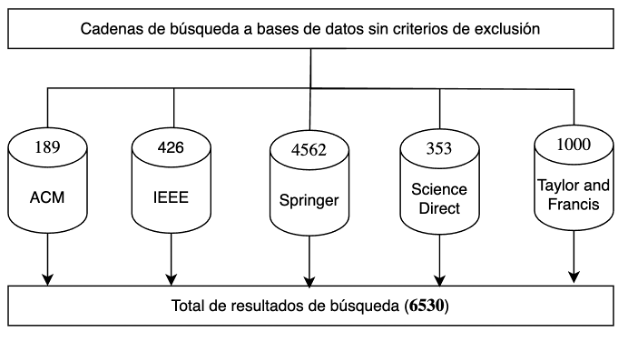
\includegraphics[scale=0.9]{tablas-images/cp2/bases-sin-criterio.png}
    \caption{Resumen de la búsqueda en bases de datos sin criterios de inclusión/exclusión}\label{fig:tabla-resumen-busqueda}
\end{figure}

\subsubsection{Aplicación de criterios de exclusión de las bases de datos}
Esta búsqueda se realizó considerando los criterios de exclusión e inclusión definidos previamente.

Las cadena de búsqueda son exactamente iguales que antes, este punto se diferencia por la aplicación de 
filtros. Para ver las capturas de pantalla veáse el apéndice B sección 2.

\subsection{Resumen de la búsqueda en bases de datos con criterios de inclusión/exclusión}\label{subsec:resumenBusquedaCriterios}

\begin{table}[H]
\centering
\scriptsize
\setlength{\tabcolsep}{4pt}
\renewcommand{\arraystretch}{1.1}
\begin{tabular}{|l|c|c|c|c|c|c|}
\hline
\textbf{Bases de datos} & \textbf{ACM} & \textbf{IEEE} & \textbf{Springer} & \textbf{Science Direct} & \textbf{Taylor \& Francis} & \textbf{Total} \\
\hline
Sin aplicar criterios & 189 & 426 & 4562 & 353 & 1000 & 6530 \\
\hline
Con criterios aplicados & 48 & 134 & 592 & 46 & 156 & 976 \\
\hline
\end{tabular}
\caption{Resumen de la búsqueda en bases de datos con criterios de inclusión/exclusión}\label{tab:resumen-busqueda}
\end{table}
\begin{figure}[H]
    \centering
    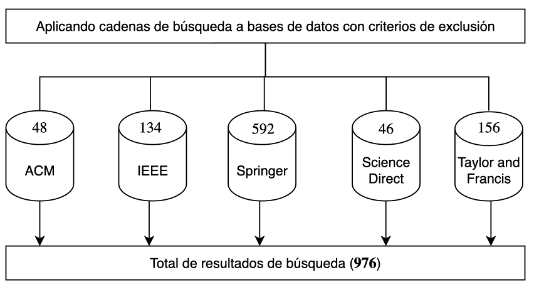
\includegraphics[scale=0.9] {tablas-images/cp2/bases-con-criterio.png}
    \caption{Resumen de la búsqueda en bases de datos con criterios de inclusión/exclusión}\label{fig:tabla-resumen-busqueda-con-criterio}
\end{figure}

\section{Eliminación de duplicados}\label{sec:eliminacionDuplicados}
La eliminación de duplicados se realizó haciendo uso de la herramienta de gestión de referencias Mendeley. Luego de obtener los artículos se agregaron a Mendeley y esta herramienta se encargó de eliminar duplicados. En este punto se eliminaron 274 artículos duplicados.

\section{Priorización de estudios}\label{sec:priorizacionEstudios}

Luego de la selección inicial de los artículos, se procedió a revisar el \textit{title}, \textit{abstract} y \textit{keywords} de cada uno. Como resultado de esta revisión, se generaron métricas de calidad para cada artículo, con el fin de priorizar aquellos más relevantes para la investigación. Las métricas utilizadas fueron las siguientes:

\begin{itemize}
    \item \textbf{SCI} (Science Citation Index)
    \item \textbf{CVI} (Core Value Index)
    \item \textbf{IRRQ} (Index Relation Research Question)
\end{itemize}

Este proceso inició con un total de 771 artículos, los cuales fueron evaluados según su alineamiento con los objetivos de la investigación. La evaluación temática permitió identificar un total de 110 artículos con una relación directa con el enfoque planteado.

\section{Estrategia de búsqueda usando bola de nieve}\label{sec:bolaDeNieve}

En esta etapa, se seleccionó el primer cuartil según el índice \textbf{IRRQ}, lo que resultó en un total de 24 artículos. Adicionalmente, se incluyeron dos artículos por criterio de inclusión directa, estableciendo así una línea base de \textbf{26 artículos}. 

Sobre esta base, se aplicó la estrategia de \textit{bola de nieve} en ambas direcciones: hacia adelante y hacia atrás. Como resultado, se obtuvieron \textbf{87 artículos} mediante la técnica hacia atrás y \textbf{495 artículos} mediante la técnica hacia adelante. 

Esto definió un nuevo conjunto de artículos para un proceso de selección adicional (\textit{screening}). En esta fase, se eliminaron \textbf{14 duplicados} y \textbf{452 artículos} fueron descartados por no estar alineados con la investigación. 

Finalmente, se obtuvo un total de \textbf{116 artículos} mediante esta estrategia de búsqueda ampliada.

\section{Diagrama de búsqueda}\label{sec:diagramaBusqueda}

\subsection{Usando cadenas de búsqueda}
En el diagrama~\ref{tab:tabla-diagrama-cadena-busqueda} se puede apreciar la estrategia de búsqueda de artículos por medio de base de datos, aplicando las cadenas de búsqueda, se consolidaron los resultados de distintas bases de datos para obtener un total de 6530 resultados, posteriormente y aplicando criterios de exclusión se redujo esta cantidad a menos de 1000 resultados. Adicional a los criterios de exclusión, también se hizo eliminación de artículos duplicados, 205 por parte del ~\textit{Reference Manager} (Mendeley), y 69 por parte del ~\textit{SMS-Builder} para un total de 274 artículos removidos. Finalmente, se realiza la etapa de screening, donde se leen las secciones claves de los artículos, como ~\textit{abstract}, ~\textit{keywords} e introducción, a través de esto se pudo descargar 671 artículos que no eran pertinentes para el estudio.
\begin{table}[H]
    \centering
    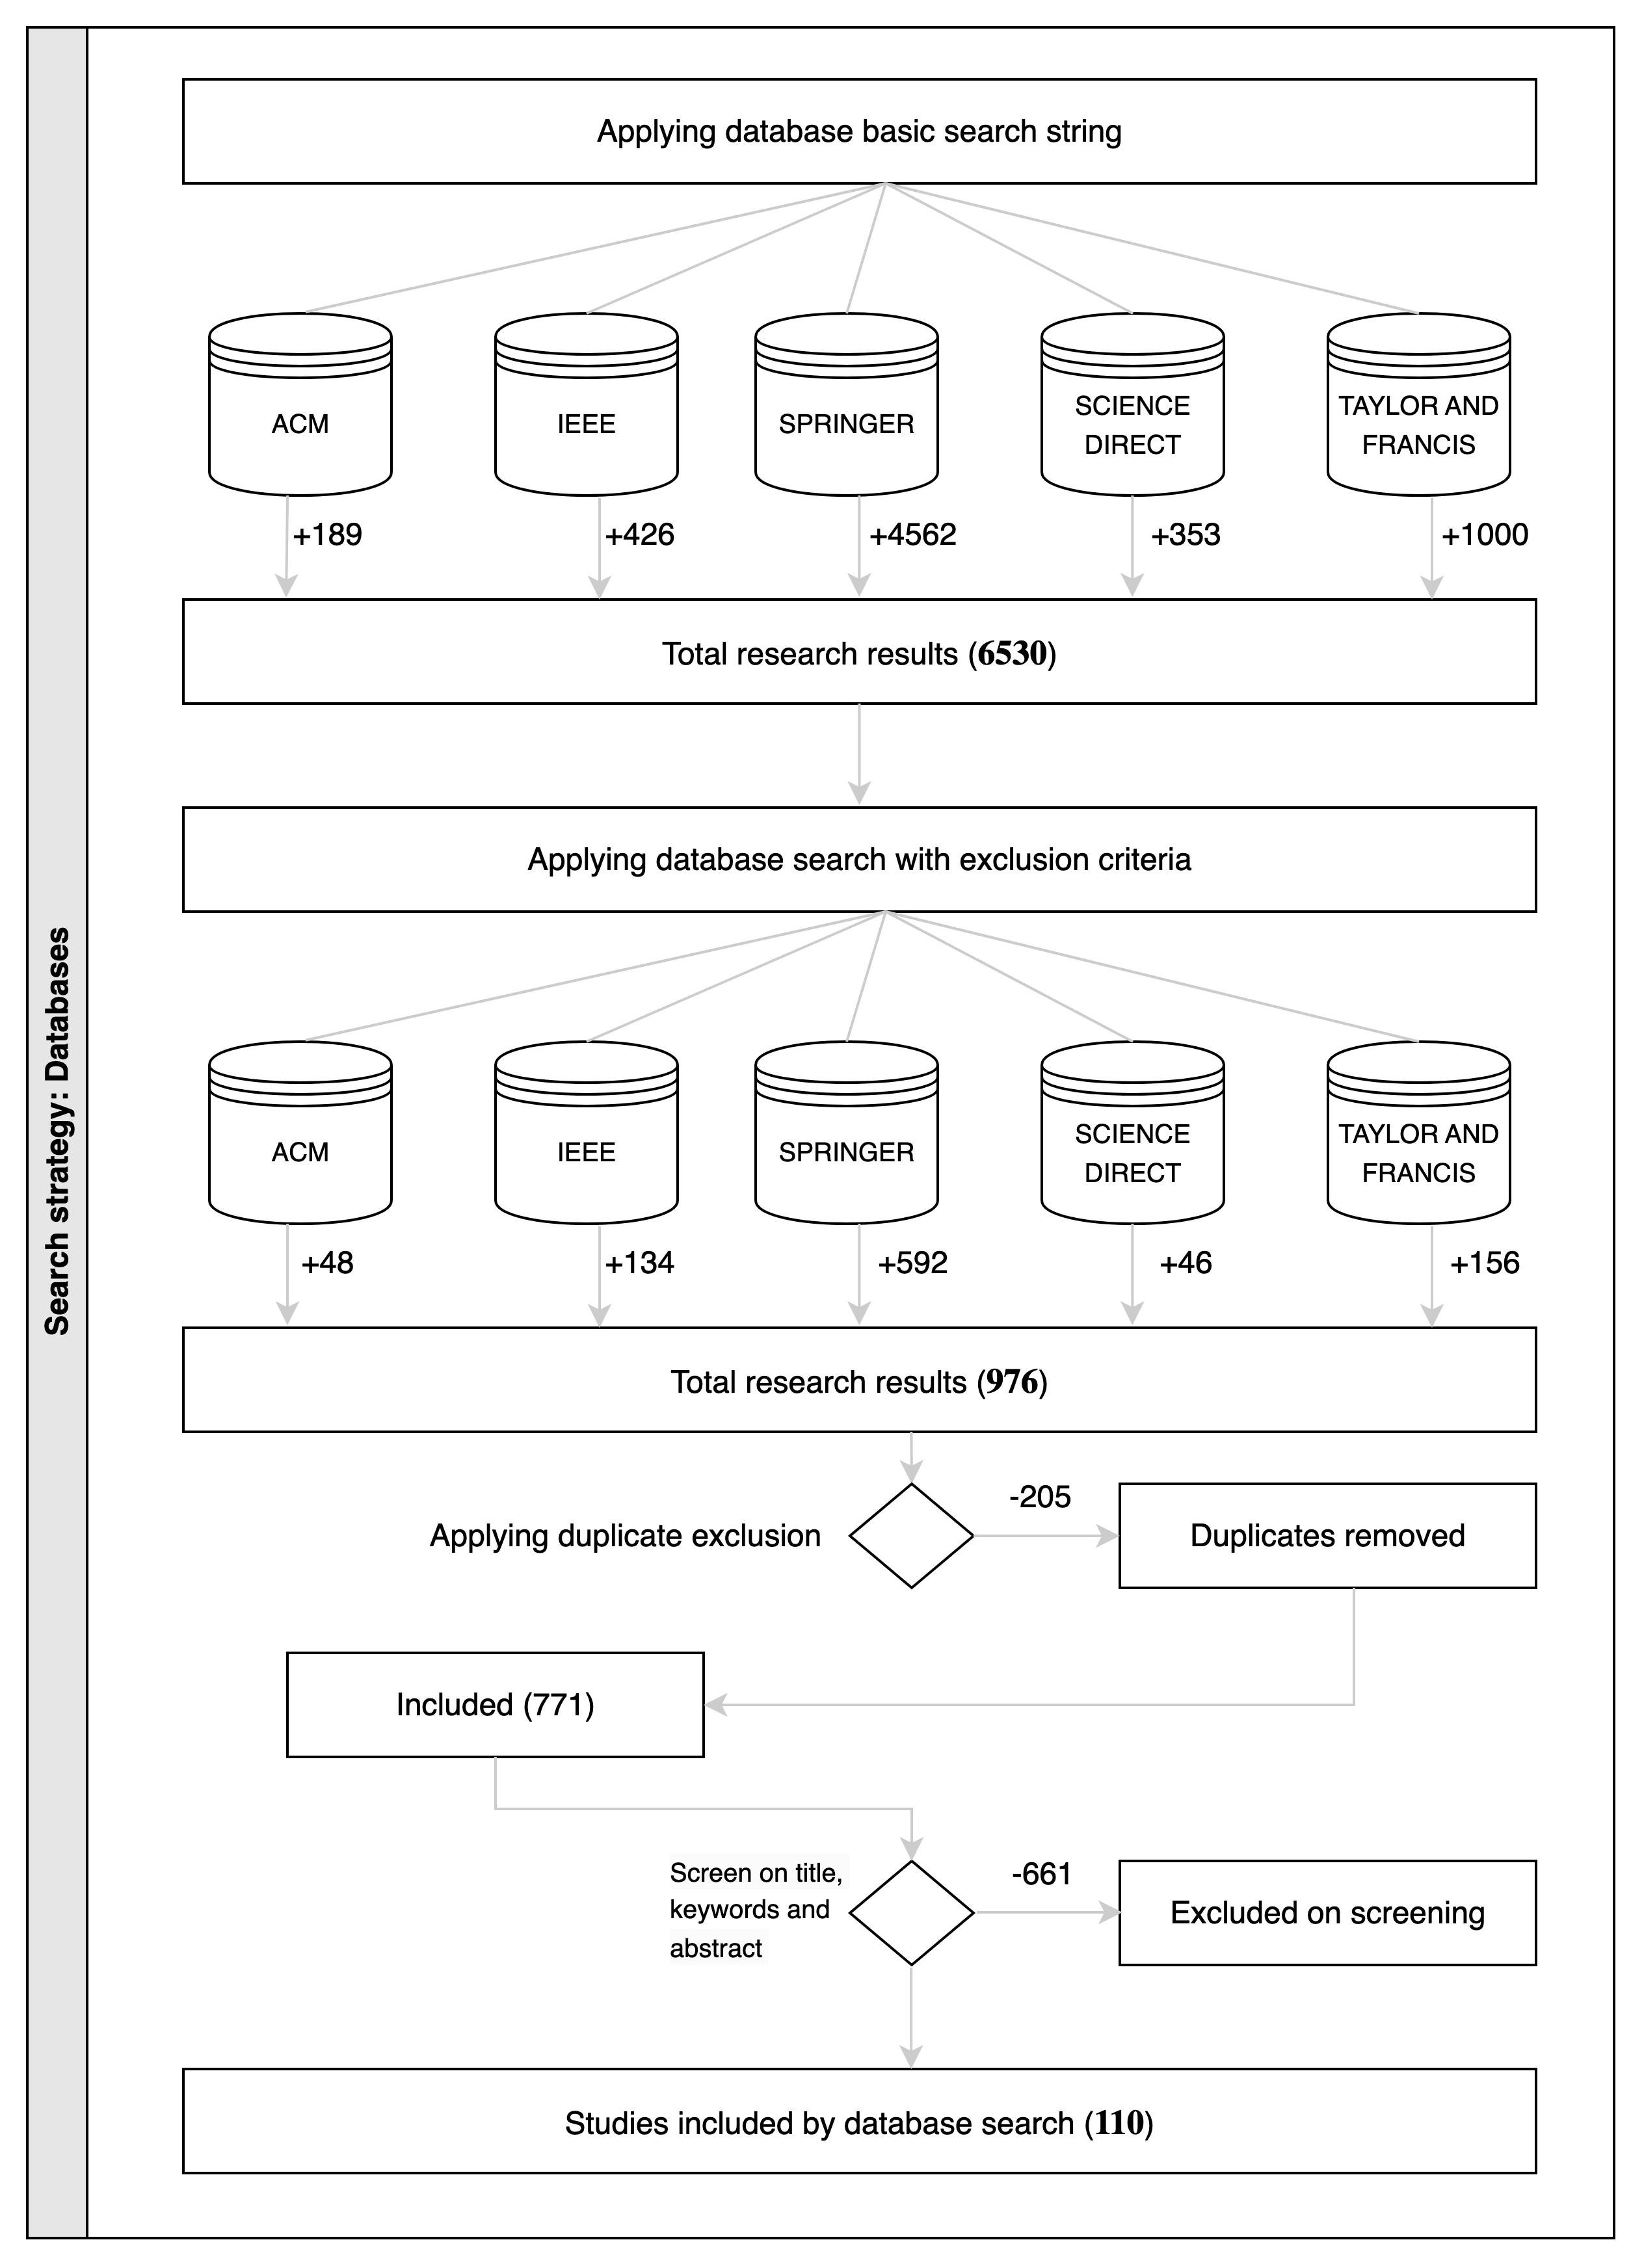
\includegraphics[scale=0.13]{tablas-images/cp2/diagrama-cadena-busqueda.png}
    \caption{Diagrama de la cadena de búsqueda}\label{tab:tabla-diagrama-cadena-busqueda}
\end{table}\label{img:busqueda-bd}

\subsection{Usando bola de nieve}
Como segunda estrategia de búsqueda dentro del SMS, se aplicó la técnica de ~\textit{Snowball}, la cual consiste en extraer artículos adicionales a partir de las referencias citadas en los estudios obtenidos en la estrategia anterior y de los estudios que citan a estos. De los 110 estudios del paso anterior, se seleccionan aquellos que tengan un SCI más relevante y se agrega uno por inclusión directa, con esto se obtiene un total de 25 artículos de línea base. Aplicando snowball hacia adelante (artículos referenciados) se obtienen 87 nuevos estudios, aplicando snowball hacia atrás (artículos que referencian el artículo base) se obtienen 495, para un total de 582. Finalmente, aplicando criterios de exclusión de remoción de duplicados y aplicando la técnica de screening, se obtiene un resultado de 116 artículos incluidos por bola de nieve. Todo este proceso se puede apreciar en la gráfica~\ref{tab:tabla-diagrama-bola-nieve-busqueda}.
\begin{table}[H]
    \centering
    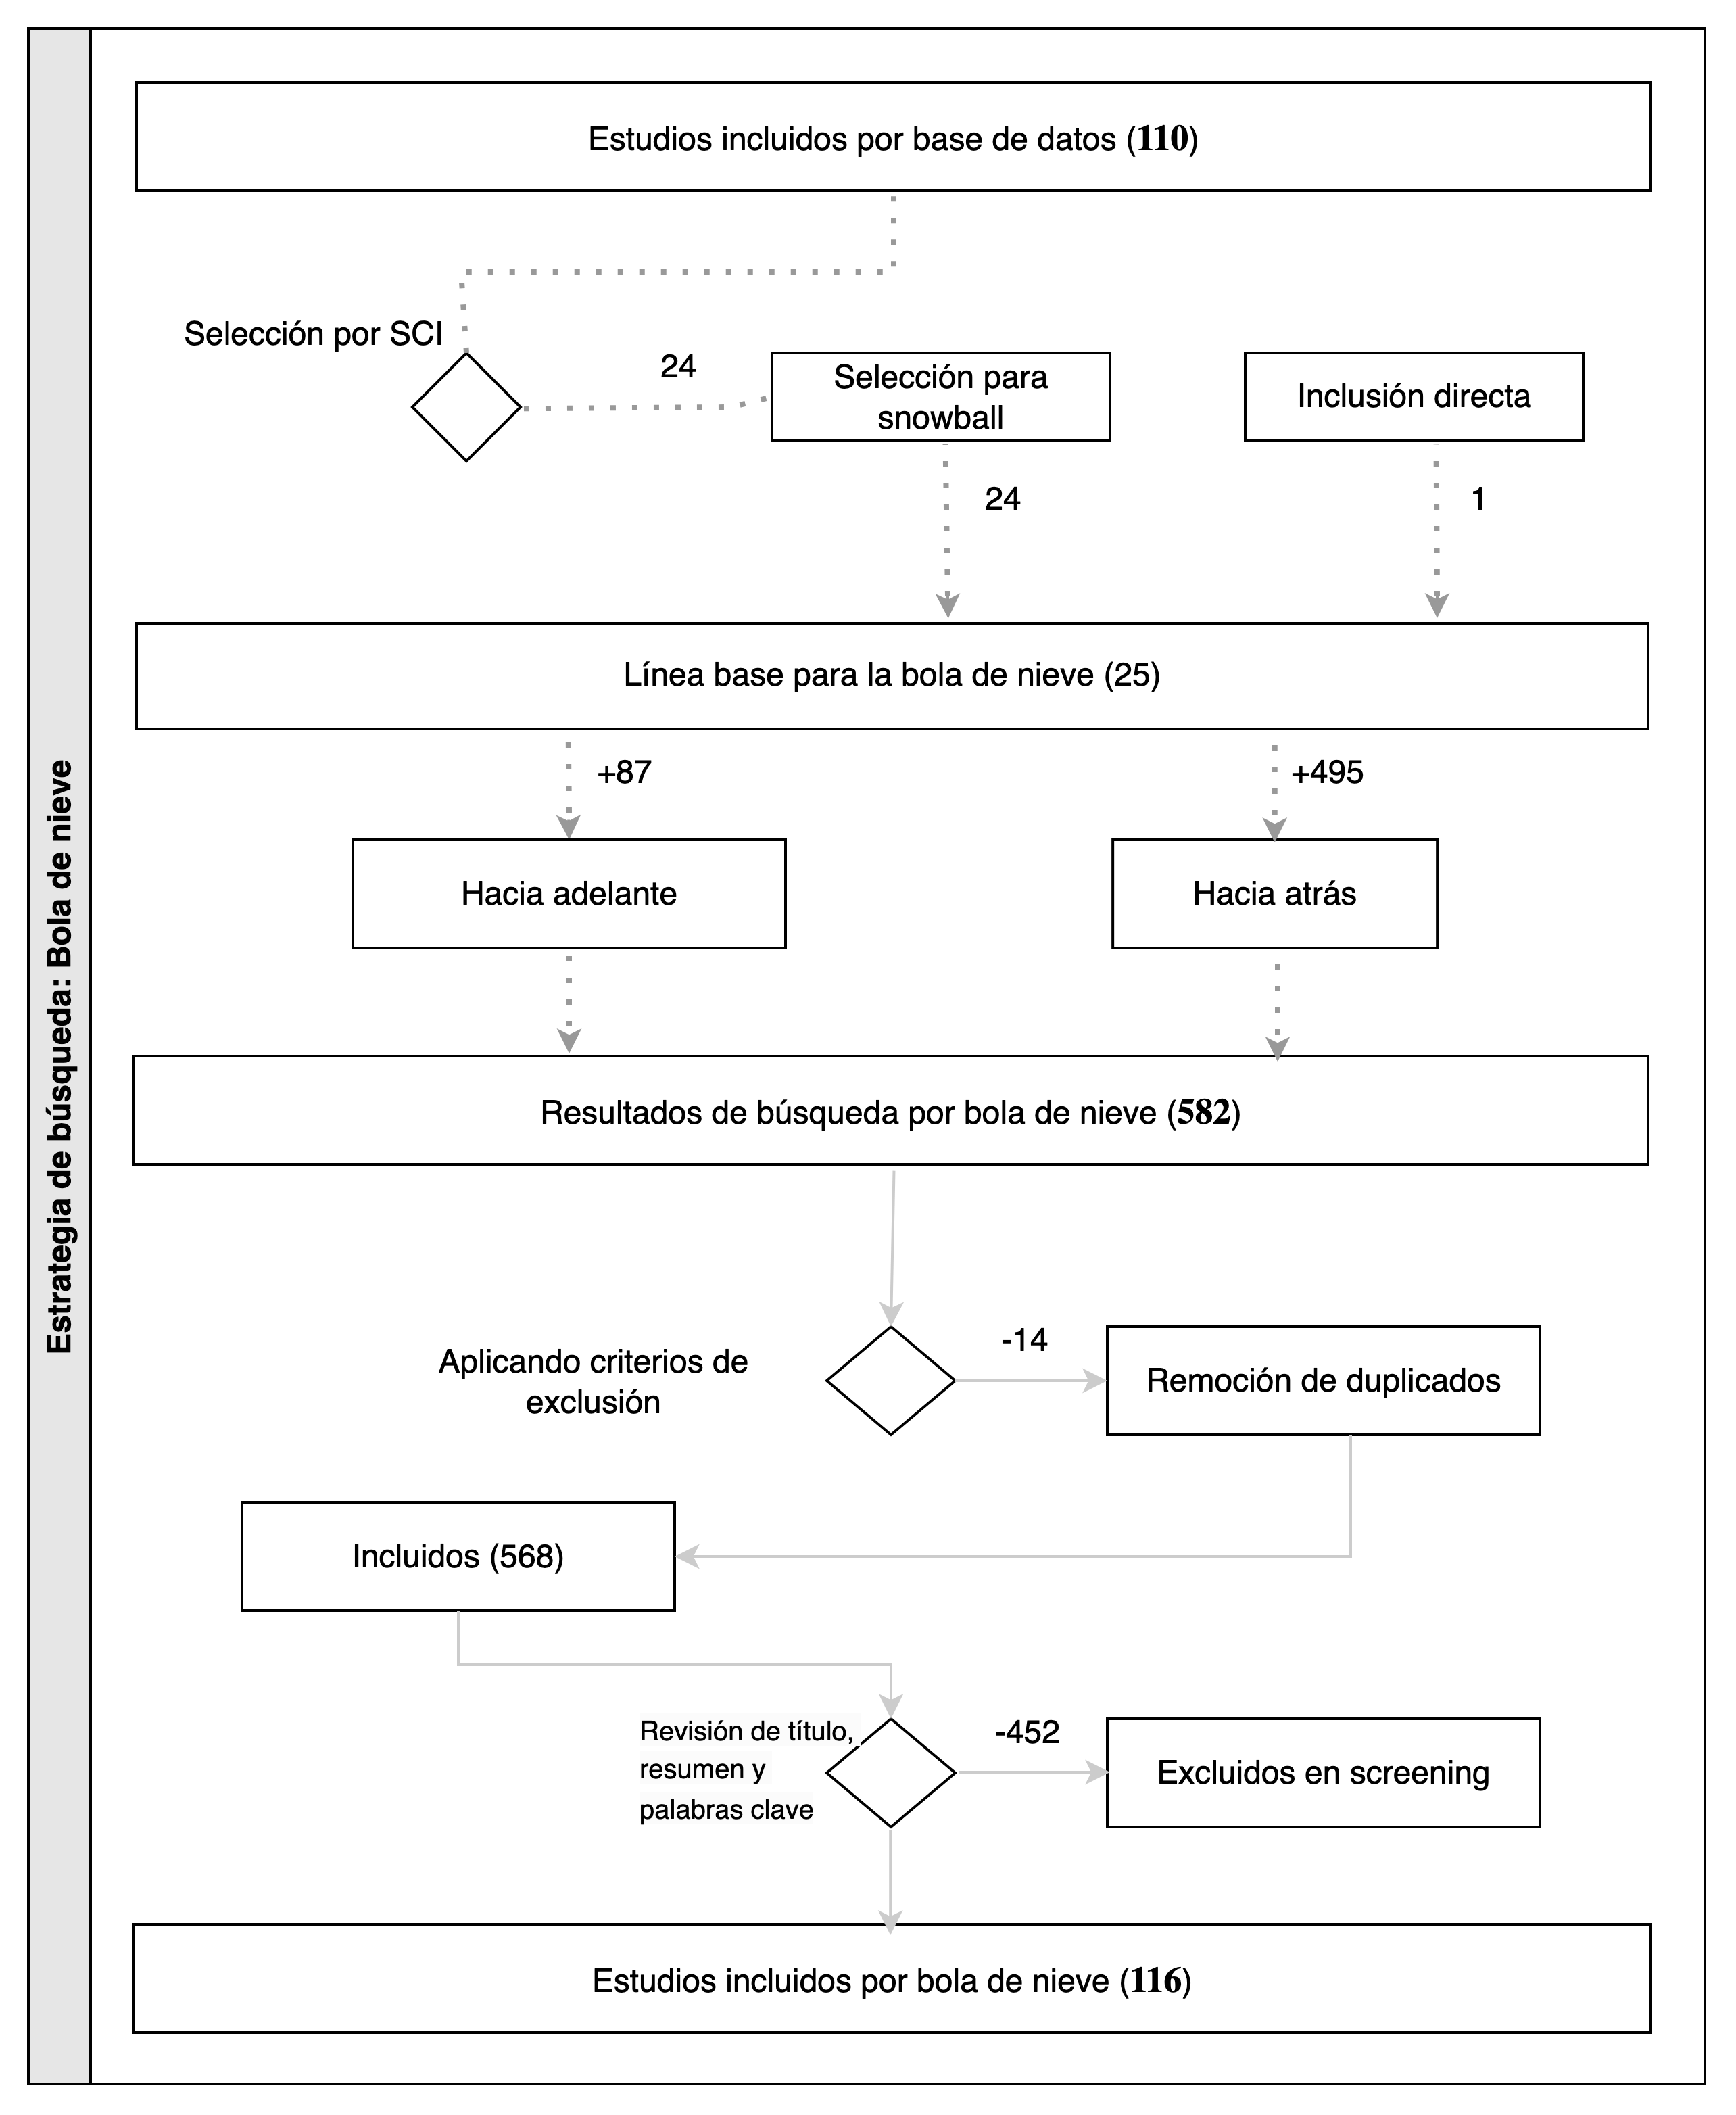
\includegraphics[scale=0.14]{tablas-images/cp2/diagrama-bola-nieve-busqueda.png}
    \caption{Diagrama de la búsqueda en bola de nieve}\label{tab:tabla-diagrama-bola-nieve-busqueda}
\end{table}

\section{Identificación de estudios}

\subsection{Artículos por año y métricas}


A continuación se presentan las gráficas que resumen los resultados de los artículos obtenidos y las estrategias anteriores.\\

En la figura~\ref{fig:diagrama-articulos-ano-metrica} se pueden visualizar las métricas de calidad, separadas por los últimos 3 años y mostrando el promedio en cada métrica de los artículos publicados en esos años, así como un apartado donde se calcula la sumatoria de estas métricas por cada año.

\begin{figure}[H]
    \centering
    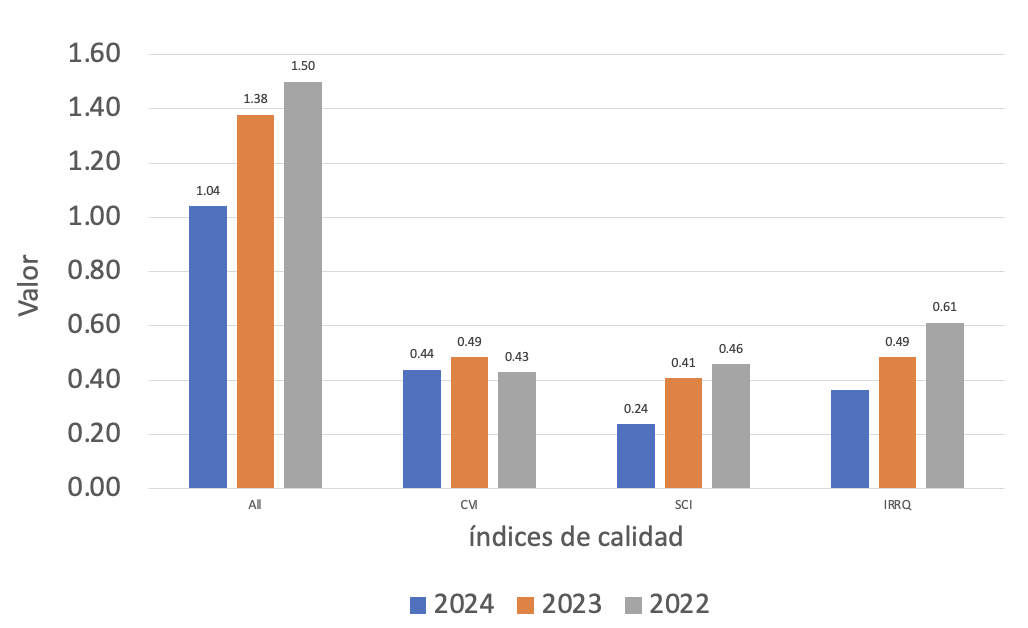
\includegraphics[scale=0.7]{tablas-images/cp2/diagrama-articulos-ano-metrica.png}
    \caption{Artículos por métricas y año}\label{fig:diagrama-articulos-ano-metrica}
\end{figure}

En la figura~\ref{fig:tipos-articulos} se muestra el conteo de artículos por su tipo específico, el cual puede ser uno de 3 opciones: 'Revista', 'Conferencia' o 'Genérico'. Vemos que la mayoría de artículos provienen de revistas.

\begin{figure}[H]
    \centering
    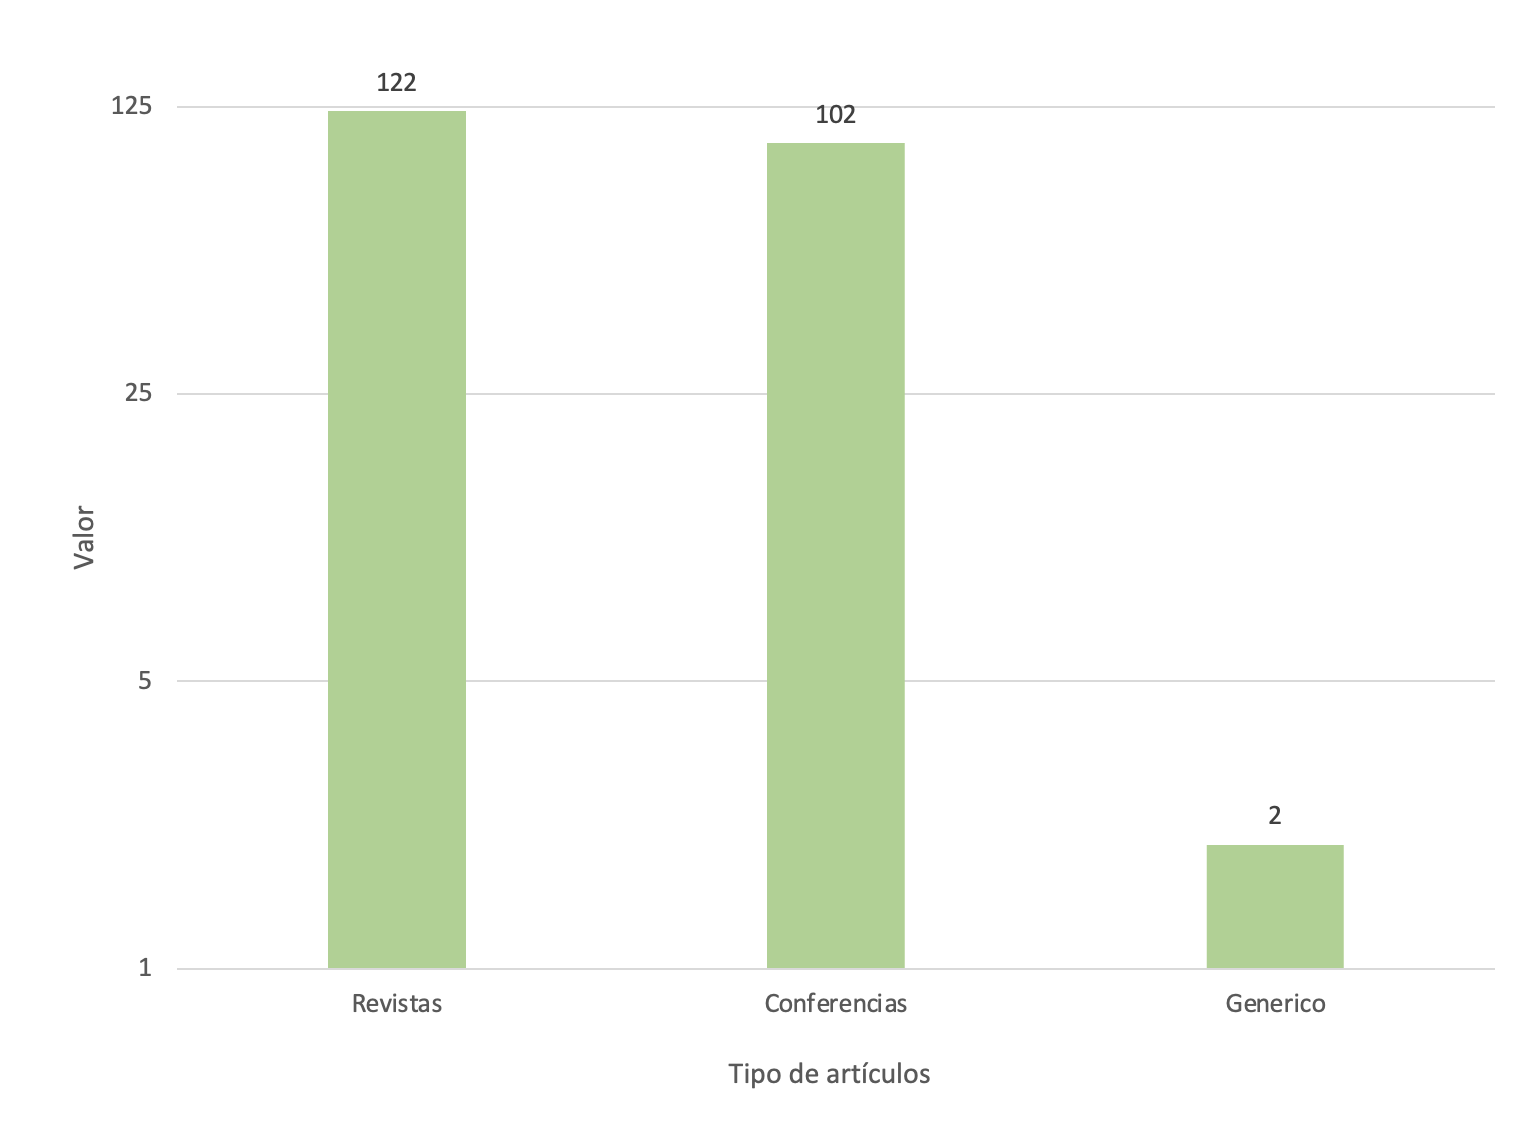
\includegraphics[scale=0.5]{tablas-images/cp2/tipos-articulos.png}
    \caption{Artículos por tipo}\label{fig:tipos-articulos}
\end{figure}

En la figura~\ref{fig:estrategia-busqueda-articulos} se detalla la cantidad de artículos que se extrajeron de cada estrategia. Se puede observar que la estrategia que generó más artículos fue la técnica de ~\textit{Snowball}.

\begin{figure}[H]
    \centering
    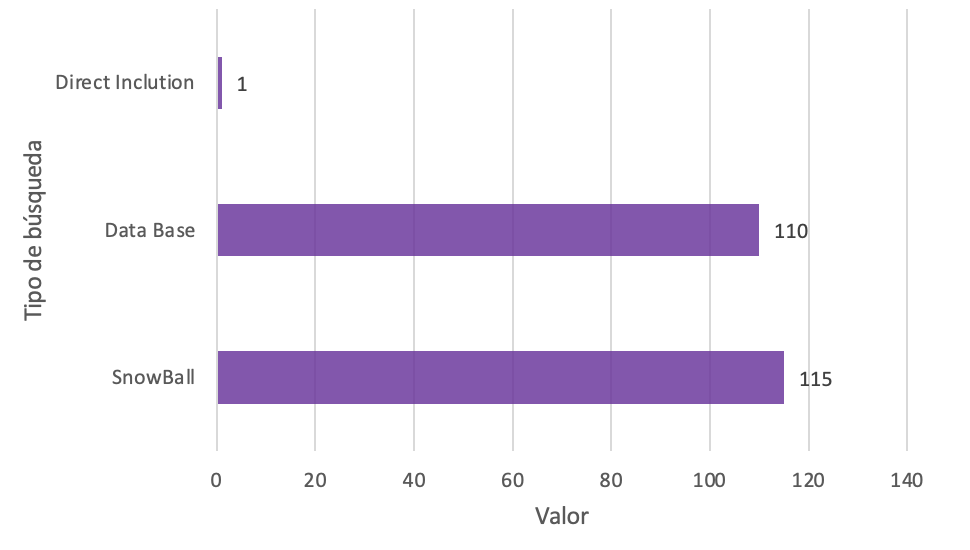
\includegraphics[scale=0.8]{tablas-images/cp2/estrategia-busqueda-articulos.png}
    \caption{Estrategia de búsqueda de artículos}\label{fig:estrategia-busqueda-articulos}
\end{figure}

Finalmente, en la figura~\ref{fig:diagrama-red-articulos} se puede apreciar un diagrama de red, que segrega por colores los tópicos más relacionados entre sí, vemos 4 grandes grupos: IA, cloud computing, virtualización, desarrollo de software.

\begin{figure}[H]
    \centering
    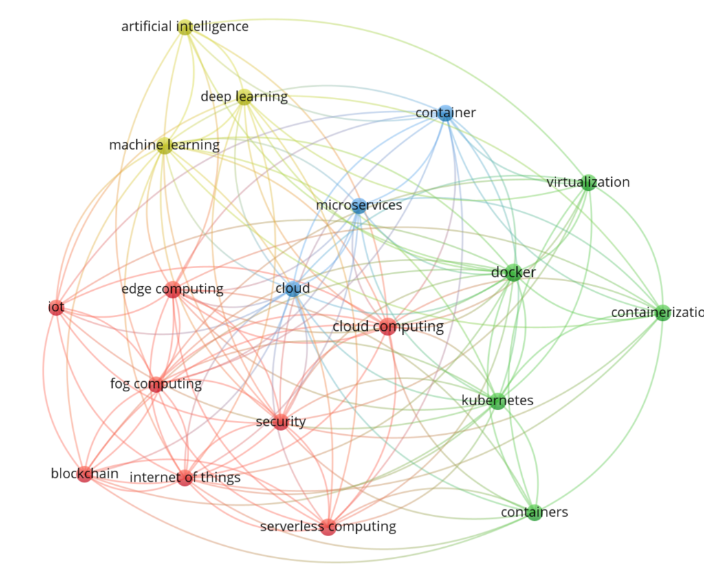
\includegraphics[scale=0.9]{tablas-images/cp2/diagrama-red-busqueda.png}
    \caption{Diagrama de red de los artículos}\label{fig:diagrama-red-articulos}
\end{figure}
\section{Información de la herramienta}

\noindent
La herramienta utilizada para este proceso de revisión de la literatura fue \textbf{SMS-BUILDER}, la cual se encuentra disponible en \textit{Docker Hub}. El estudio realizado puede consultarse en el siguiente enlace:

\begin{center}
\href{https://sms-vbc.iti.grid.uniquindio.edu.co/}{\texttt{https://sms-vbc.iti.grid.uniquindio.edu.co/}}
\end{center}

\noindent
Adicionalmente, se implementaron procesos de respaldo como medida de seguridad. Estos \textit{backups} fueron almacenados en ubicaciones diferentes, siguiendo la estrategia de respaldo \textbf{3--2--1}.

\section{Nichos de mercado}

\subsection{Docker}
Docker se posiciona principalmente en el nicho de mercado de desarrolladores de software, empresas tecnológicas y proveedores de servicios en la nube que buscan una solución para la creación, implementación y gestión de aplicaciones en contenedores \citep{Hill2025}. Su capacidad de automatizar despliegues y garantizar la portabilidad entre entornos lo convierte en una opción ideal para DevOps y desarrollo ágil \citep{Mag2025}.

\subsection{Podman}
Podman está orientado a entornos empresariales y desarrolladores que requieren una solución de contenerización sin \textit{daemon}, compatible con OCI y con enfoque en la seguridad \citep{Surendhar2024}. Su naturaleza sin \textit{daemon} y su capacidad para ejecutar contenedores de forma aislada permiten su adopción en entornos donde la seguridad y la conformidad son prioridades \citep{Trevor2022}.

\subsection{Udocker}
Udocker se especializa en nichos de mercado académicos y de investigación, donde los usuarios necesitan ejecutar contenedores sin privilegios en sistemas que no permiten la instalación de software de nivel de sistema \citep{Campos2017}. Su facilidad para funcionar en entornos HPC (Computación de Alto Rendimiento) sin requerir permisos de root lo hace adecuado para instituciones de investigación \citep{Gomes2018}.

\subsection{Wasm (WebAssembly)}
Wasm se centra en el nicho de desarrollo web y aplicaciones de alto rendimiento en el navegador \citep{Haas2017}. Su capacidad para ejecutar código de forma eficiente en múltiples plataformas, incluidas aplicaciones de escritorio y móviles, lo convierte en una opción atractiva para empresas de desarrollo de software que buscan optimización multiplataforma \citep{Jangda2019}.

\subsection{LXC (Linux Containers)}
LXC es popular en entornos de virtualización ligera y servidores, donde se requiere un control granular sobre los entornos de contenedores \citep{Silva2024}. Su uso está orientado a proveedores de alojamiento web, desarrolladores de software y administradores de sistemas que necesitan un control preciso del entorno del sistema operativo \citep{Simon2023}.

\subsection{Containerd}
Containerd está dirigido a proveedores de servicios en la nube y plataformas de orquestación como Kubernetes, donde se requiere una solución de gestión de contenedores ligera y compatible con OCI \citep{Vano2023}. Su arquitectura modular lo convierte en una opción preferida para grandes infraestructuras \citep{Zhou2021}.

\subsection{LXD}
LXD se enfoca en nichos de mercado que requieren entornos de virtualización basados en contenedores que imiten máquinas virtuales, como proveedores de servicios en la nube, plataformas de pruebas y entornos de desarrollo \citep{Silva2024}. Su capacidad para ofrecer entornos de sistema completo lo hace ideal para desarrolladores y administradores de sistemas \citep{Kaiser2022}.

\subsection{Rkt}
Rkt fue diseñado para satisfacer las necesidades de proveedores de servicios en la nube y organizaciones que buscan una alternativa a Docker con un enfoque en la seguridad y compatibilidad OCI \citep{Lingayat2018}. Aunque su desarrollo ha sido discontinuado, sigue siendo relevante en entornos donde la compatibilidad y la seguridad son críticas \citep{Watada2019}.

\subsection{Singularity}
Singularity se centra en entornos de computación científica y HPC, donde se requiere portabilidad de aplicaciones sin necesidad de privilegios de root \citep{10.1145/3332186.3332192}. Es ampliamente adoptado en universidades, centros de investigación y laboratorios que ejecutan aplicaciones de alto rendimiento \citep{Kurtzer2017}.

\subsection{runC}
runC está orientado a proveedores de servicios en la nube, plataformas de orquestación como Kubernetes y desarrolladores de software que buscan una solución de contenedorización ligera y compatible con OCI \citep{Perez2005}. Su adopción en proyectos de gran escala se debe a su eficiencia y cumplimiento de estándares de contenedores \citep{151962df5f7e4b9faba0629540c11439}.

\subsection{CRI-O}
CRI-O está diseñado específicamente para su integración con Kubernetes, sirviendo como un motor de contenedores ligero y compatible con OCI para esta plataforma \citep{CNCF2019}. Es una solución ideal para proveedores de servicios en la nube y organizaciones que utilizan Kubernetes como su plataforma de orquestación principal \citep{151962df5f7e4b9faba0629540c11439}.

\subsection{Hyper-V Containers}
Hyper-V Containers están orientados a empresas que utilizan infraestructuras basadas en Windows, ofreciendo una solución de contenedorización segura y eficiente para aplicaciones basadas en Windows \citep{Smith2016}. Su integración con el ecosistema de Microsoft lo hace ideal para empresas con infraestructuras híbridas \citep{Clark2024}.

\subsection{OpenVZ}
OpenVZ se centra en proveedores de alojamiento web y servicios VPS, donde se requiere una solución de virtualización ligera basada en contenedores que permita un control granular sobre los recursos del sistema y la administración de múltiples instancias \citep{OpenVZ2015}.

\subsection{Linux VServer}
Linux VServer está orientado a administradores de sistemas y proveedores de servicios que requieren una solución de virtualización ligera basada en contenedores para la administración de servidores seguros y eficientes \citep{10.1145/1272996.1273025}. Es una opción adecuada para entornos de servidor dedicados y alojamientos compartidos \citep{LinuxVirt2017}.

\subsection{Google gVisor}
Google gVisor está dirigido a proveedores de servicios en la nube y organizaciones que priorizan la seguridad en sus entornos de contenedores \citep{LopezFalcon2024}. Su arquitectura de \textit{sandbox} proporciona un aislamiento fuerte, lo que lo convierte en una opción atractiva para aplicaciones sensibles \citep{gvisor2025}.

\subsection{Kata Containers}
Kata Containers se centra en entornos donde se requiere un alto nivel de seguridad y aislamiento, como proveedores de servicios en la nube y empresas que manejan información confidencial \citep{Viktorsson2020}. Su capacidad para combinar la eficiencia de los contenedores con el aislamiento de máquinas virtuales es su principal ventaja \citep{10.1145/1272996.1273025}.

\subsection{Firecracker}
Firecracker está orientado a proveedores de servicios en la nube y plataformas de cómputo en la nube que requieren micro VMs eficientes y seguras \citep{Jain}. Es una solución ideal para plataformas \textit{serverless} y entornos multi-tenant \citep{246288}.

\subsection{Sarus}
Sarus está dirigido a entornos de HPC y computación científica, donde los usuarios necesitan ejecutar contenedores de forma segura en sistemas de alto rendimiento \citep{Sarus2021}. Su compatibilidad con estándares de contenedores y su enfoque en la seguridad lo hacen ideal para centros de investigación y universidades \citep{B2020}.


\begin{table}[H]
\centering
\scriptsize
\setlength{\tabcolsep}{3pt}
\renewcommand{\arraystretch}{1.1}
\begin{tabular}{|>{\centering\arraybackslash}m{0.18\textwidth}| 
                >{\centering\arraybackslash}m{0.25\textwidth}| 
                >{\centering\arraybackslash}m{0.20\textwidth}| 
                >{\centering\arraybackslash}m{0.25\textwidth}|}
\hline
\textbf{Tecnologías} & \textbf{Licencias} & \textbf{Términos de uso} & \textbf{Costo} \\
\hline
Docker & Apache 2.0 & \href{https://www.docker.com/legal/docker-terms-service/}{link} & \$11-\$24 \\
\hline
Podman & Apache 2.0 & \href{https://github.com/containers/podman/blob/main/LICENSE}{link} & Gratis \\
\hline
Udocker & Apache 2.0 & \href{https://github.com/indigo-dc/udocker/blob/master/LICENSE}{link} & Gratis \\
\hline
Wasm & Apache 2.0 & \href{https://github.com/WebAssembly/design/blob/main/LICENSE}{link} & Gratis \\
\hline
LXC & GNU LGPLv2.1+ & \href{https://linuxcontainers.org/lxc/introduction/}{link} & Gratis \\
\hline
Containerd & Apache 2.0 & \href{https://github.com/containerd/containerd/blob/main/LICENSE}{link} & Gratis \\
\hline
LXD & AGPL-3.0 & \href{https://github.com/canonical/lxd}{link} & Gratis \\
\hline
Rkt & Apache 2.0 & \href{https://github.com/rkt/rkt/blob/master/LICENSE}{link} & Descontinuado \\
\hline
Singularity & BSD 3-Clause & \href{https://github.com/sylabs/singularity/blob/main/LICENSE.md}{link} & CE: Gratis, PRO: \$30/año \\
\hline
runC & Apache 2.0 & \href{https://github.com/opencontainers/runc/blob/main/LICENSE}{link} & Gratis \\
\hline
CRI-O & Apache 2.0 & \href{https://github.com/cri-o/cri-o/blob/main/LICENSE}{link} & Gratis \\
\hline
Hyper-V containers & Windows Propietaria & \href{https://learn.microsoft.com/es-es/virtualization/windowscontainers/images-eula}{link} & \$1,176 USD \\
\hline
OpenVZ & GPL v2 & \href{https://openvz.org/}{link} & Gratis \\
\hline
Linux VServer & GPL v2 & \href{http://linux-vserver.org/}{link} & Gratis \\
\hline
Google gVisor & Apache 2.0 & \href{https://github.com/google/gvisor}{link} & Gratis \\
\hline
Kata Containers & Apache 2.0 & \href{https://github.com/kata-containers/kata-containers/blob/main/LICENSE}{link} & Gratis \\
\hline
Firecracker & Apache 2.0 & \href{https://github.com/firecracker-microvm/firecracker}{link} & Gratis \\
\hline
Sarus & BSD 3-Clause & \href{https://github.com/eth-cscs/sarus}{link} & Gratis \\
\hline
\end{tabular}
\caption{Comparativa de tecnologías de contenerización, licencias, términos de uso y costos}
\end{table}

En la tabla~\ref{tab:interfaz-vbc} se puede ver la interfaz de uso por cada tecnología. Como se puede apreciar, la gran mayoría de tecnologías se utilizan a través de una CLI (línea de comandos). Esto, en muchos casos, puede implicar un aumento en la curva de aprendizaje, pero mayor facilidad para gestionar y automatizar las tecnologías una vez que se ha comprendido el uso de su interfaz.
\begin{table}[H]
\centering
\scriptsize
\setlength{\tabcolsep}{3pt}
\renewcommand{\arraystretch}{1.1}
\begin{tabularx}{\textwidth}{|p{0.18\textwidth}|>{\raggedright\arraybackslash}X|}
\hline
\textbf{Tecnología} & \textbf{Interfaz de Uso} \\
\hline
Docker & \CLI\ principalmente, con Docker Desktop para interfaz gráfica. \\
\hline
Podman & \CLI\ similar a Docker, sin daemon. Opcional Podman Desktop. \\
\hline
Udocker & \CLI\ específica para ejecutar contenedores sin privilegios root. \\
\hline
Wasm  & Ejecución través de navegadores web, \API\ de JavaScript. \\
\hline
LXC & \CLI\ mediante comando lxc, sin interfaz gráfica oficial. \\
\hline
Containerd & \CLI\ con herramientas como ctr, backend para otras herramientas. \\
\hline
LXD & \CLI\ mediante lxd/lxc, con interfaz web LXD Web \UI. \\
\hline
Rkt & \CLI\ mediante comandos como rkt run (descontinuado). \\
\hline
Singularity & \CLI\ mediante comandos singularity para gestión de contenedores. \\
\hline
runC & \CLI\ mediante comandos runc, runtime bajo Docker y Kubernetes. \\
\hline
CRI-O & \CLI, interactúa con Kubernetes, sin interfaz gráfica dedicada. \\
\hline
Hyper-V containers & \CLI\ (PowerShell) o Hyper-V Manager para VMs. \\
\hline
OpenVZ & \CLI\ mediante comandos vzctl, con interfaces gráficas de terceros. \\
\hline
Linux VServer & \CLI\ mediante comandos vserver para gestión. \\
\hline
Google gVisor & \CLI\ mediante comandos estándar de Docker con seguridad adicional. \\
\hline
Kata Containers & \CLI\ mediante kata-runtime, integración con Kubernetes. \\
\hline
Firecracker & \CLI\ mediante \API\ RESTful y herramientas firecracker. \\
\hline
Sarus & \CLI\ mediante comando sarus para entornos \HPC. \\
\hline
\end{tabularx}
\caption{Interfaz de uso de cada VBC}\label{tab:interfaz-vbc}
\end{table}

En el cuadro~\ref{tab:integracion-cloud-vbc} se puede ver la integración a las distintas plataformas cloud que tiene cada tecnología. Se puede ver que muchas tecnologías tienen integración directa con 3 de los proveedores cloud más famosos, a saber: AWS, GCP y Azure. Algunas tecnologías, por otro lado, solo soportan implementación de nubes privadas, como LXD.
\begin{table}[H]
\centering
\scriptsize
\setlength{\tabcolsep}{3pt}
\renewcommand{\arraystretch}{1.1}
\begin{tabularx}{\textwidth}{|p{0.2\textwidth}|X|}
\hline
\textbf{Tecnología} & \textbf{Integración con Proveedores de Cloud} \\
\hline
Docker & Integración con \AWS\ (ECR, ECS), Google Cloud (GCR, GKE), Azure (ACR, AKS), y otros proveedores a través de herramientas como Docker Compose, Docker Swarm y Docker Desktop. \\
\hline
Podman & Compatible con \AWS\ (ECR), Google Cloud (GCR), Azure (ACR), aunque su integración con orquestadores como Kubernetes es más reciente y menos prevalente que Docker. \\
\hline
Udocker & Generalmente se usa en entornos sin privilegios de root y en plataformas como \HPC\ . No tiene una integración directa con proveedores de nube a gran escala. \\
\hline
Wasm (WebAssembly) & Integración principalmente con servicios de computación en la nube como \AWS\ Lambda, Google Cloud Functions, y Azure Functions, ya que permite la ejecución eficiente de código en la nube sin dependencia del sistema operativo subyacente. \\
\hline
LXC & Se puede integrar en plataformas de nube privada y algunas soluciones híbridas. Se usa en servidores de nube como OpenStack, pero no tiene una integración directa con plataformas públicas principales. \\
\hline
Containerd & Integración fuerte con Kubernetes, que a su vez se integra con proveedores de nube como \AWS\ (EKS), Google Cloud (GKE), Azure (AKS) y otros. \\
\hline
LXD & Puede integrarse con plataformas de nube privada, como OpenStack, para ofrecer contenedores ligeros que emulan máquinas virtuales. No tiene integración directa con los proveedores de nube pública principales, pero puede ser utilizado en soluciones personalizadas. \\
\hline
Rkt & Aunque estaba integrado con Kubernetes y otras plataformas, su descontinuación limita la integración con proveedores de nube. En el pasado, soportaba plataformas como \AWS\ y Google Cloud. \\
\hline
Singularity & Utilizado principalmente en entornos de computación científica y HPC. Puede integrarse con proveedores como \AWS\ (HPC, Batch) y Google Cloud (Compute Engine) para tareas específica de alto rendimiento. \\
\hline
runC & Integración con Kubernetes, que se usa ampliamente en proveedores de nube como \AWS\ (EKS), Google Cloud (GKE), y Azure (AKS) para la orquestación de contenedores. \\
\hline
CRI-O & Integración directa con Kubernetes, lo que le permite ser utilizado en proveedores de nube como \AWS\ (EKS), Google Cloud (GKE), Azure (AKS), y otros servicios de orquestación de contenedores. \\
\hline
Hyper-V containers & Integración exclusiva con Microsoft Azure, especialmente con Azure Kubernetes Service (AKS) y otras soluciones basadas en Hyper-V. \\
\hline
OpenVZ & Tradicionalmente usado en proveedores de hosting como OVH, aunque su uso ha disminuido frente a soluciones más modernas. La integración con nubes públicas es limitada y generalmente personalizada. \\
\hline
Linux VServer & Utilizado principalmente en proveedores de hosting dedicados y servidores privados, sin integración directa con proveedores de nube pública como \AWS\, Google Cloud o Azure. \\
\hline
Google gVisor & Integración con Google Cloud, especialmente en Google Kubernetes Engine (GKE), para agregar una capa adicional de seguridad a los contenedores. \\
\hline
Kata Containers & Soporta proveedores de nube pública como \AWS\, Google Cloud, y Azure a través de Kubernetes, proporcionando aislamiento similar a máquinas virtuales en entornos de contenedores. \\
\hline
\end{tabularx}
\caption{Integración cloud de cada VBC}
\label{tab:integracion-cloud-vbc}
\end{table}

\section{Cuadrante Gartner}
Para visualizar el panorama de las tecnologias de contenerización en cuanto a su relevancia en la industria, se aplicó un cuadrante gartner, el cual mide dos dimensiones, Visión y Ejecución, es decir que tan buena proyeccion puede tener la tecnologia en el futuro y que tan bien se desempeña actualmente en el corto plazo.

\begin{table}[H]
\centering
\scriptsize
\setlength{\tabcolsep}{4pt}
\renewcommand{\arraystretch}{1.0}
\begin{tabular}{|p{0.3\textwidth}|c|c|p{0.25\textwidth}|}
\hline
\textbf{Tecnología} & \textbf{Visión (X)} & \textbf{Ejecución (Y)} & \textbf{Cuadrante} \\
\hline
Docker & 9 & 9 & Líderes \\
\hline
Containerd & 8 & 8 & Líderes \\
\hline
Podman & 8 & 7 & Retadores \\
\hline
CRI-O & 7 & 7 & Retadores \\
\hline
LXC & 6 & 6 & Jugadores de Nicho \\
\hline
LXD & 6 & 6 & Jugadores de Nicho \\
\hline
Udocker & 4 & 4 & Jugadores de Nicho \\
\hline
runC & 5 & 5 & Jugadores de Nicho \\
\hline
Rkt & 3 & 4 & Jugadores de Nicho \\
\hline
Singularity & 5 & 4 & Visionarios \\
\hline
Wasm & 9 & 5 & Visionarios \\
\hline
Google gVisor & 8 & 6 & Visionarios \\
\hline
Kata Containers & 7 & 6 & Visionarios \\
\hline
Firecracker & 8 & 6 & Visionarios \\
\hline
Sarus & 4 & 4 & Jugadores de Nicho \\
\hline
Hyper-V containers & 5 & 5 & Jugadores de Nicho \\
\hline
OpenVZ & 4 & 5 & Jugadores de Nicho \\
\hline
Linux VServer & 3 & 4 & Jugadores de Nicho \\
\hline
\end{tabular}
\caption{Tabla de medición para el cuadrante gartner}
\label{tab:cuadrante-gartner}
\end{table}

Una vez hecha la tabla anterior, se pueden resumir los resultados en el diagrama~\ref{fig:tabla-cuadrante-gartner}, que representa el cuadrante Gartner. Se pueden ver 4 grandes grupos de tecnologías dependiendo de su nivel de visión y ejecución: Líderes, Retadores, Visionarios, Jugadores de nicho.
\begin{figure}[H]
    \centering
    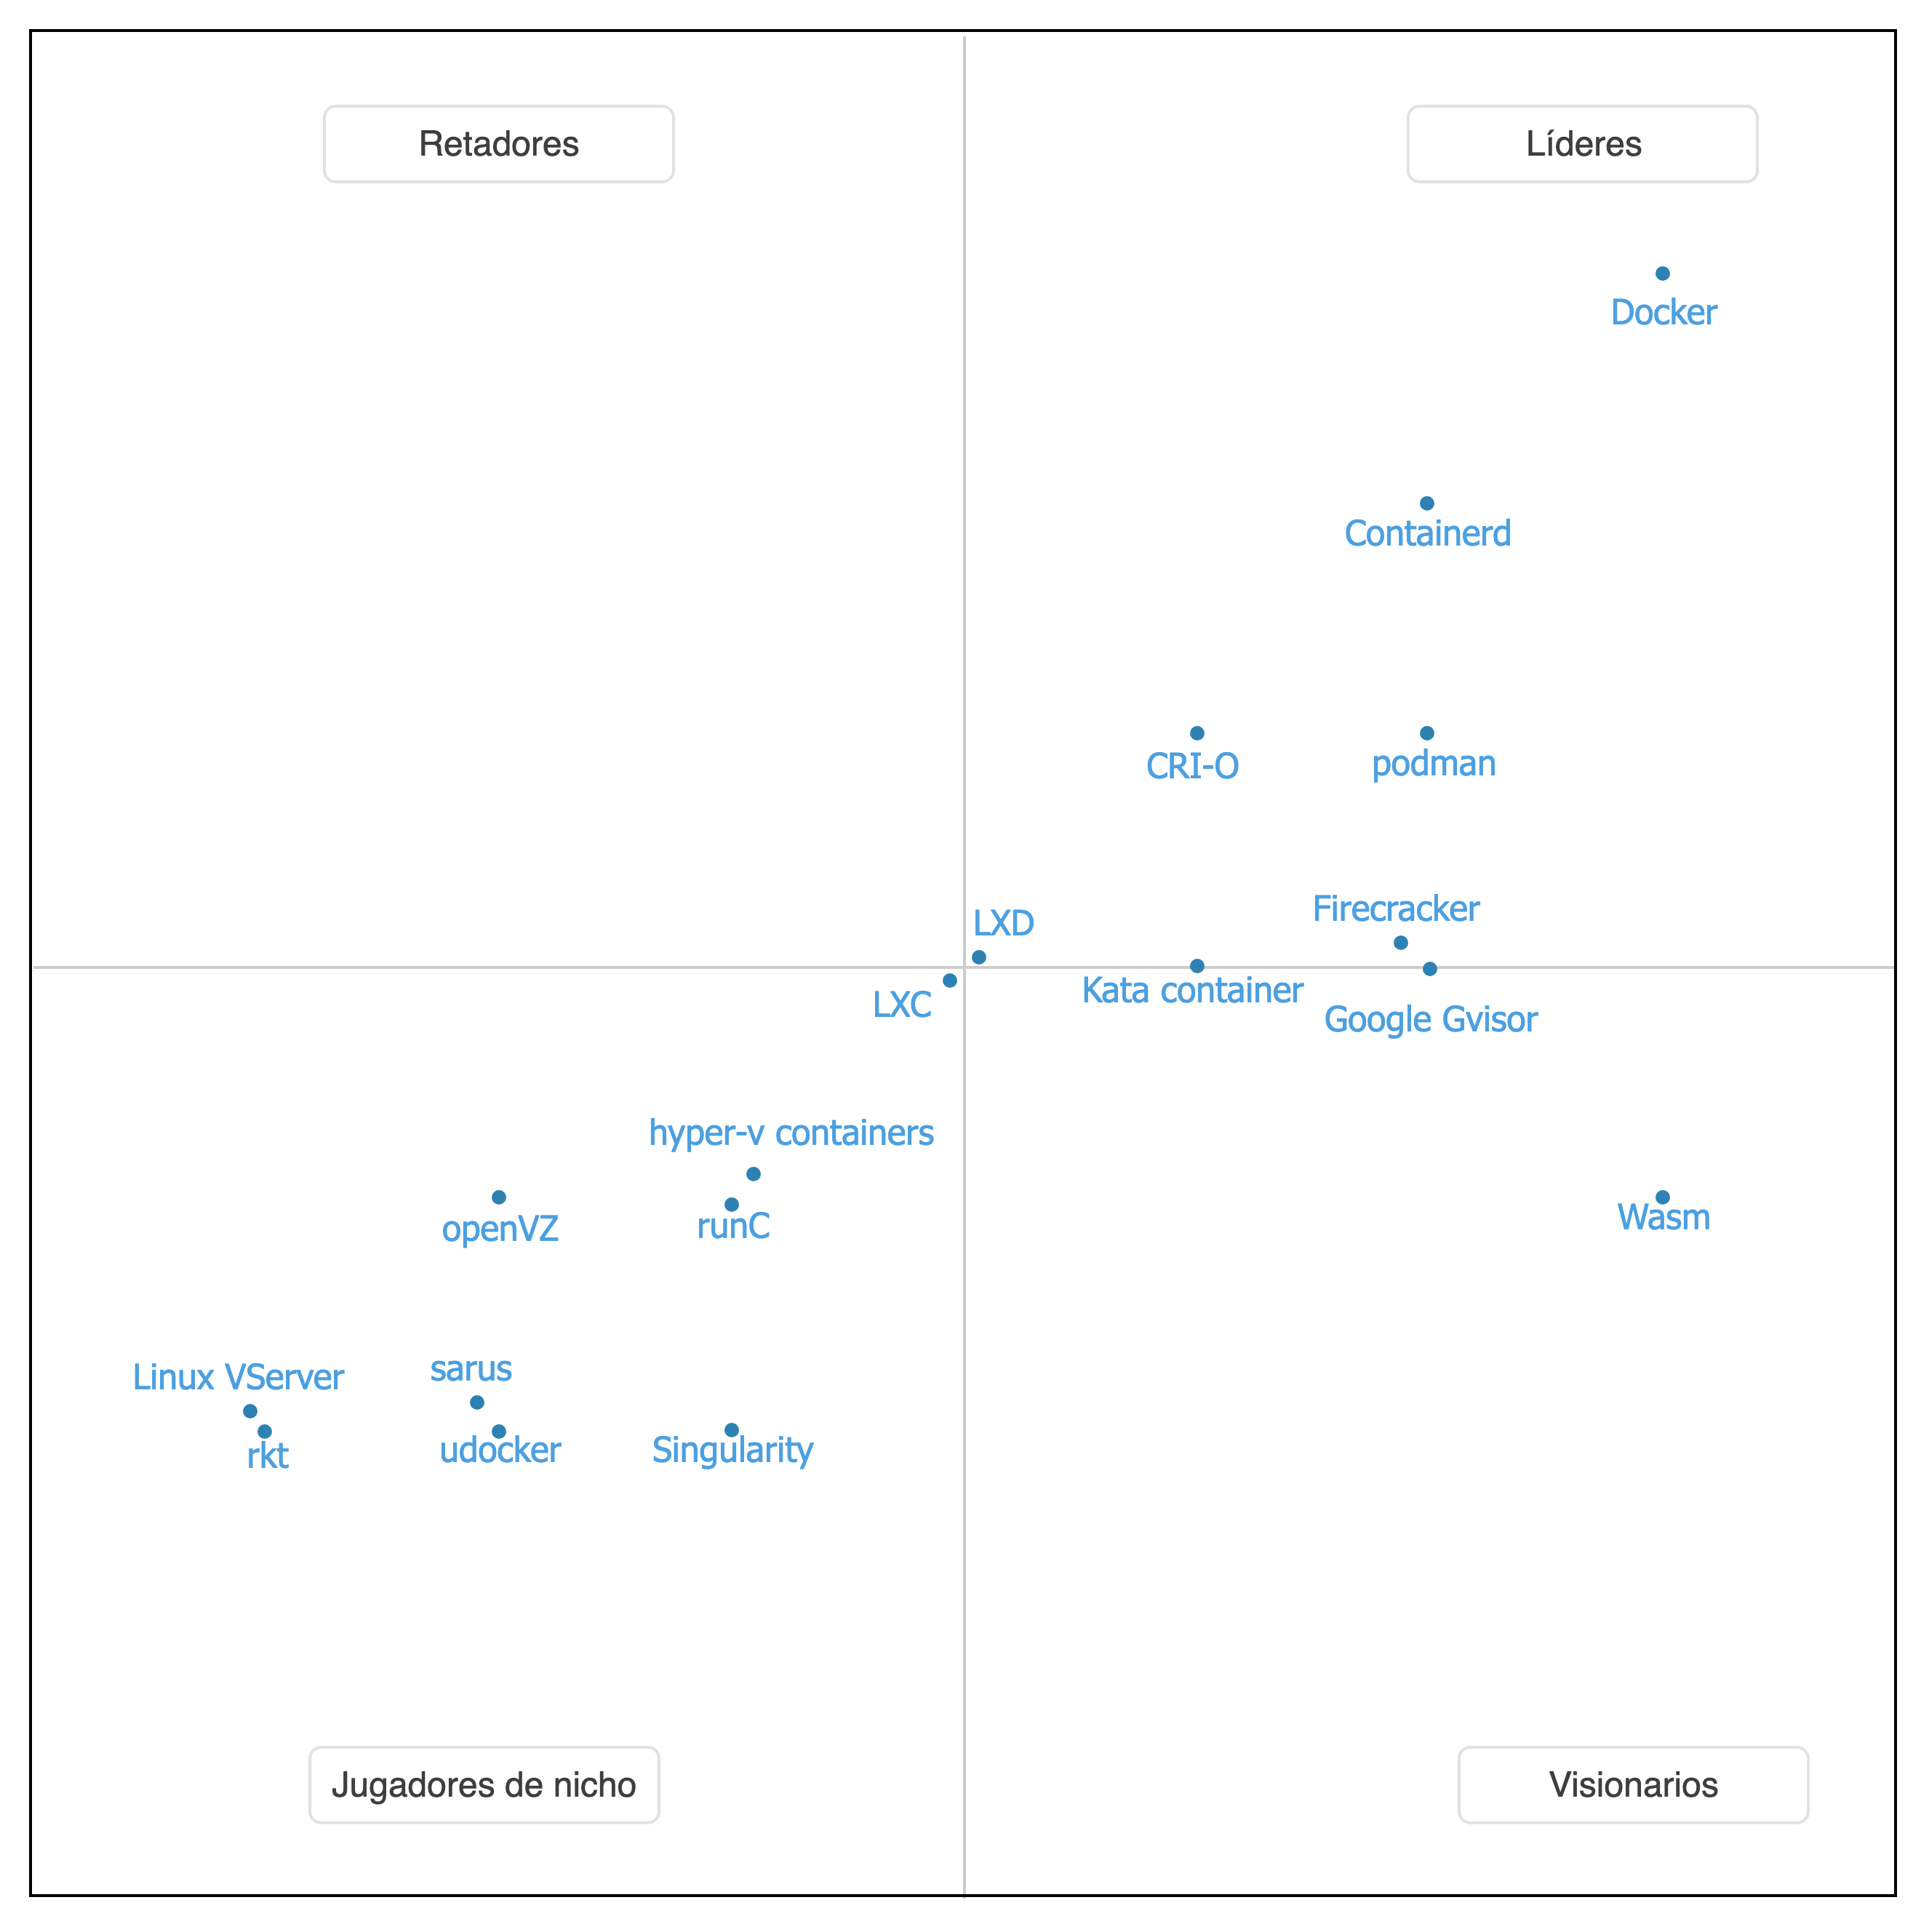
\includegraphics[width=\textwidth] {tablas-images/cp3/cuadrante-gartner.png}
    \caption{Cuadrante de Gartner de cada VBC}\label{fig:tabla-cuadrante-gartner}
\end{figure}

En la tabla~\ref{tab:entornos-ejecucion-vbc} se puede ver los sistemas operativos en los que se ejecutan estas tecnologias, se puede ver que la mayoria de estas estan diseñadas para sistemas linux, seguido de sistemas windows y por ultimo sistemas macOS, en cuyo caso las 2 unicas tecnologias que soportan este SO son ~\textit{Docker} y ~\textit{Podman}.
\begin{table}[H]
\centering
\scriptsize
\setlength{\tabcolsep}{3pt}
\renewcommand{\arraystretch}{1.1}
\begin{tabularx}{\textwidth}{|p{0.2\textwidth}|X|}
\hline
\textbf{Tecnología} & \textbf{Ambiente de Ejecución} \\
\hline
Docker & Sistemas Linux, Windows y macOS. Entornos de desarrollo, pruebas y producción, incluyendo la nube pública (\AWS, Google Cloud, Azure). \\
\hline
Podman & Sistemas Linux y macOS, con soporte experimental en Windows. Usado en entornos de desarrollo y producción sin necesidad de un daemon. \\
\hline
Udocker & Sistemas Linux, en entornos de computación de alto rendimiento (\HPC) y servidores compartidos, permitiendo ejecutar contenedores sin privilegios de root. \\
\hline
Wasm (WebAssembly) & Navegadores web (Chrome, Firefox, Safari, Edge). Ejecución en aplicaciones web y entornos de alto rendimiento sin dependencia del sistema operativo subyacente. \\
\hline
LXC & Sistemas Linux. Utilizado para crear contenedores ligeros que actúan como máquinas virtuales, con aplicaciones aisladas en servidores y plataformas de nube privada. \\
\hline
Containerd & Sistemas Linux y Windows. Usado en plataformas de orquestación como Kubernetes, y en infraestructuras de contenedores a gran escala. \\
\hline
LXD & Sistemas Linux. Virtualización ligera de contenedores como máquinas virtuales completas, ideal para servidores y plataformas de virtualización en la nube privada. \\
\hline
Rkt & Sistemas Linux. Anteriormente usado en entornos de orquestación de contenedores y en infraestructuras de nube privada. (Descontinuado actualmente). \\
\hline
Singularity & Sistemas Linux, especialmente en entornos de computación científica y \HPC\ . Portabilidad de aplicaciones científicas sin necesidad de privilegios de root. \\
\hline
runC & Sistemas Linux. Runtime ligero de contenedores compatible con los estándares de la Open Container Initiative (\OCI), utilizado por plataformas como Docker y Kubernetes. \\
\hline
CRI-O & Sistemas Linux. Integrado con Kubernetes para la gestión eficiente de contenedores en plataformas de orquestación en la nube y servidores locales. \\
\hline
Hyper-V containers & Sistemas Windows (Windows Server y Windows 10 con Hyper-V habilitado). Usado para contenedores con aislamiento mediante micro-VMs, ideal para entornos híbridos. \\
\hline
OpenVZ & Sistemas Linux. Virtualización a nivel de contenedor en proveedores de hosting para ofrecer entornos aislados y eficientes. \\
\hline
Linux VServer & Sistemas Linux. Contenedores que funcionan como servidores virtuales, usados en entornos de hosting y administración de servidores de alta disponibilidad. \\
\hline
Google gVisor & Plataformas de nube, especialmente Google Cloud. Capa adicional de seguridad para contenedores en entornos multitenant. \\
\hline
Kata Containers & Sistemas Linux. Virtualización ligera con aislamiento similar a máquinas virtuales, utilizado en plataformas de contenedores en la nube y servidores donde se requiere seguridad. \\
\hline
Firecracker & Plataformas de computación en la nube, como \AWS\ . Optimizado para micro-VMs ultra ligeras y de alto rendimiento en entornos serverless. \\
\hline
Sarus & Sistemas Linux. Entornos de computación de alto rendimiento (\HPC) y clústeres de supercomputación, proporcionando portabilidad y eficiencia sin privilegios de root. \\
\hline
\end{tabularx}
\caption{Entornos de ejecución de cada VBC}
\label{tab:entornos-ejecucion-vbc}
\end{table}

En el cuadro~\ref{tab:matriz-dofa} se define una matriz DOFA, especificando las debilidades, oportunidades, fortalezas y amenazas de las tecnologías VBC. Esto permite tener varios aspectos en cuenta a la hora de seleccionar una tecnología o realizar una implementación.
\begin{table}[H]
\centering
\scriptsize
\setlength{\tabcolsep}{4pt}
\renewcommand{\arraystretch}{1.2}
\begin{tabularx}{\textwidth}{|X|X|}
\hline
\textbf{Fortalezas} & \textbf{Oportunidades} \\
\hline
\begin{minipage}[t]{\linewidth}
\vspace{2pt}
\begin{itemize}
    \setlength\itemsep{0pt}
    \setlength\parskip{0pt}
    \setlength\parsep{0pt}
    \item La VBC es ampliamente utilizada en plataformas en la nube como AWS, Azure y Google Cloud.
    \item Herramientas como Kubernetes y Docker se actualizan constantemente, agregando nuevas funcionalidades y mejoras.
    \item Numerosos foros, grupos y organizaciones están dedicados a mejorar y desarrollar soluciones de contenerización.
    \item Los contenedores pueden ejecutarse en múltiples entornos (local, nube, híbrido).
    \item Permiten una mejor utilización de recursos en comparación con las máquinas virtuales tradicionales.
\end{itemize}
\vspace{2pt}
\end{minipage}
&
\begin{minipage}[t]{\linewidth}
\vspace{2pt}
\begin{itemize}
    \setlength\itemsep{0pt}
    \setlength\parskip{0pt}
    \setlength\parsep{0pt}
    \item Los contenedores son ligeros y comparten el kernel del sistema operativo, reduciendo el consumo de recursos.
    \item Una aplicación en contenedor puede ejecutarse en cualquier entorno compatible sin modificaciones.
    \item Permiten implementar y gestionar aplicaciones de manera escalable y eficiente.
    \item Los contenedores permiten que las aplicaciones se ejecuten de manera independiente, evitando conflictos entre ellas.
    \item Herramientas como Docker Compose y Kubernetes facilitan la gestión automatizada de contenedores.
\end{itemize}
\vspace{2pt}
\end{minipage}
\\
\hline
\textbf{Debilidades} & \textbf{Amenazas} \\
\hline
\begin{minipage}[t]{\linewidth}
\vspace{2pt}
\begin{itemize}
    \setlength\itemsep{0pt}
    \setlength\parskip{0pt}
    \setlength\parsep{0pt}
    \item Los contenedores comparten el mismo núcleo del sistema operativo host, lo que podría permitir que una vulnerabilidad afecte a todos los contenedores.
    \item A medida que crece la infraestructura, gestionar múltiples contenedores y sus redes se vuelve complejo.
    \item A diferencia de las máquinas virtuales tradicionales, los contenedores son efímeros por diseño, lo que complica el manejo de datos persistentes.
    \item No todos los sistemas y aplicaciones son compatibles de manera nativa con contenedores, lo que requiere configuraciones específicas.
    \item La seguridad y rendimiento de los contenedores están directamente relacionados con el sistema operativo subyacente.
\end{itemize}
\vspace{2pt}
\end{minipage}
&
\begin{minipage}[t]{\linewidth}
\vspace{2pt}
\begin{itemize}
    \setlength\itemsep{0pt}
    \setlength\parskip{0pt}
    \setlength\parsep{0pt}
    \item Si no se aplican buenas prácticas, los contenedores pueden ser vulnerables a ataques.
    \item El uso de soluciones propietarias como AWS o Azure puede generar dependencia tecnológica.
    \item Las tecnologías de contenerización evolucionan rápidamente, lo que puede dejar obsoletas algunas soluciones.
    \item Un mal diseño puede llevar a un consumo ineficiente de recursos.
    \item Aunque existen buenas prácticas, no hay una regulación estándar única para la gestión de contenedores.
\end{itemize}
\vspace{2pt}
\end{minipage}
\\
\hline
\end{tabularx}
\caption{Tabla de matriz DOFA para el cuadrante gartner}
\label{tab:matriz-dofa}
\end{table}
\begin{table}[H]
\centering
\rowcolors{2}{gray!10}{white}
\begin{tabularx}{\textwidth}{>{\raggedright\arraybackslash}X >{\raggedright\arraybackslash}X}
\rowcolor{gray!30}
\textbf{Tecnología} & \textbf{Enlace a la Documentación} \\

Docker & \href{https://docs.docker.com/}{link} \\
Podman & \href{https://podman.io/docs}{link} \\
Udocker & \href{https://github.com/indigo-dc/udocker}{link} \\
Wasm (WebAssembly) & \href{https://webassembly.org/docs/faq/}{link} \\
LXC & \href{https://linuxcontainers.org/incus/docs/main/}{link} \\
Containerd & \href{https://containerd.io/docs/}{link} \\
LXD & \href{https://linuxcontainers.org/incus/docs/main/}{link} \\
Rkt & \href{https://github.com/rkt/rkt}{link} \\
Singularity & \href{https://docs.sylabs.io/guides/4.3/user-guide/}{link} \\
runC & \href{https://github.com/opencontainers/runc}{link} \\
CRI-O & \href{https://github.com/cri-o/cri-o}{link} \\
Hyper-V containers & \href{https://docs.microsoft.com/en-us/virtualization/windowscontainers/}{link} \\
OpenVZ & \href{https://openvz.org/}{link} \\
Linux VServer & \href{http://linux-vserver.org/Documentation}{link} \\
Google gVisor & \href{https://gvisor.dev/docs/}{link} \\
Kata Containers & \href{https://katacontainers.io/docs/}{link} \\
Firecracker & \href{https://firecracker-microvm.github.io/}{link} \\
Sarus & \href{https://github.com/eth-cscs/sarus}{link} \\

\end{tabularx}
\caption{Enlaces a la documentación de tecnologías de contenerización}
\end{table}
\ChapterImageStar[cap:benchmarking]{Benchmarking}{./images/fondo.png}\label{cap:benchmarking}

\section{Definición de las pruebas}

Para evaluar el rendimiento de distintas tecnologías de contenerización —específicamente Docker, Podman, LXC, LXD y Containerd— se diseñó un conjunto de pruebas orientadas a medir aspectos clave del desempeño en entornos controlados. Las pruebas incluyeron el consumo de CPU y memoria RAM, el tiempo de arranque de los contenedores, el \textit{throughput} de red y la latencia de acceso a disco. 

Para garantizar la repetibilidad y objetividad de los resultados, se desarrollaron scripts en \textit{Bash} que automatizan la ejecución de cada métrica en condiciones homogéneas. Estas pruebas permiten comparar las tecnologías evaluadas bajo criterios cuantificables y facilitar un análisis técnico de sus capacidades en escenarios reales de uso.

\section{Construcción de las pruebas}

La construcción de las pruebas se llevó a cabo mediante el desarrollo de scripts automatizados en \textit{Bash}, diseñados para ejecutarse de forma uniforme sobre cada tecnología de contenerización evaluada. Cada script fue responsable de iniciar contenedores, ejecutar cargas de trabajo específicas y recolectar métricas de rendimiento relevantes.

Para medir el consumo de CPU y memoria RAM, se utilizó \texttt{pidstat}, una utilidad que permite la medición del consumo de recursos. El tiempo de arranque se determinó midiendo el intervalo entre la orden de inicio del contenedor y el momento en que estuvo completamente operativo. 

Para evaluar el \textit{throughput} de red se emplearon herramientas como \texttt{iperf}, mientras que la latencia de disco fue medida utilizando \texttt{fio}. Todas las pruebas fueron ejecutadas múltiples veces para reducir el impacto de variaciones puntuales y asegurar la confiabilidad de los resultados. Los scripts fueron programados para ejecutarse 10 veces; al final se extrae un promedio y este constituye el puntaje final de la tecnología de contenerización en cuestión.

En el repositorio \underline{\href{https://github.com/Anubis-1001/benchmark-tecnologias-de-contenerizacion} {\texttt{ GitHub benchmarking}}} se pueden encontrar los scripts resultantes de este proceso.

\section{Resultados de las pruebas}

Los resultados obtenidos a partir de las pruebas evidencian diferencias significativas en el rendimiento entre las tecnologías de contenerización evaluadas. Estos se pueden consultar en el archivo de Excel \underline{\href{https://docs.google.com/spreadsheets/d/1Ce37Sm3Swyfa88Ur1yQbLarq_D86obUIAGGJocgQbUE/edit?usp=sharing} {\texttt{benchmarking\_tecnologias}}}.

En términos de consumo de CPU, Docker y Containerd presentan las mejores métricas; en consumo de memoria RAM, LXC y LXD mostraron un mejor uso de los recursos. En cuanto al tiempo de arranque, Containerd destacó por su velocidad, seguido de cerca por Docker, mientras que LXC presentó un arranque considerablemente más lento en comparación con las demás tecnologías.

Para el \textit{throughput} de red, todas las tecnologías mostraron un desempeño comparable, siendo LXC el más destacado; no obstante, Podman quedó muy por debajo en esta métrica. Finalmente, en la medición de latencia de disco, LXD y Containerd obtuvieron los mejores resultados, lo que sugiere una gestión de E/S más directa y liviana.

Estos resultados permiten establecer un panorama claro de fortalezas y debilidades de cada solución, según el tipo de carga o entorno de ejecución esperado.

\section{Métricas de rendimiento}

De la ejecución de las pruebas se obtuvieron las siguientes métricas de rendimiento:

\begin{figure}[H]
    \centering
    \includegraphics[scale=0.5] {tablas-images/cp4/cpu.png}
    \caption{Métricas de uso de CPU}\label{fig:tabla-metricas-cpu}
\end{figure}
\begin{figure}[H]
    \centering
    \includegraphics[width=\textwidth] {tablas-images/cp4/ram.png}
    \caption{Métricas de uso de RAM}\label{fig:tabla-metricas-ram}
\end{figure}
\begin{figure}[H]
    \centering
    \includegraphics[width=\textwidth] {tablas-images/cp4/io.png}
    \caption{Métricas de entrada/salida}\label{fig:tabla-metricas-io}
\end{figure}
\begin{figure}[H]
    \centering
    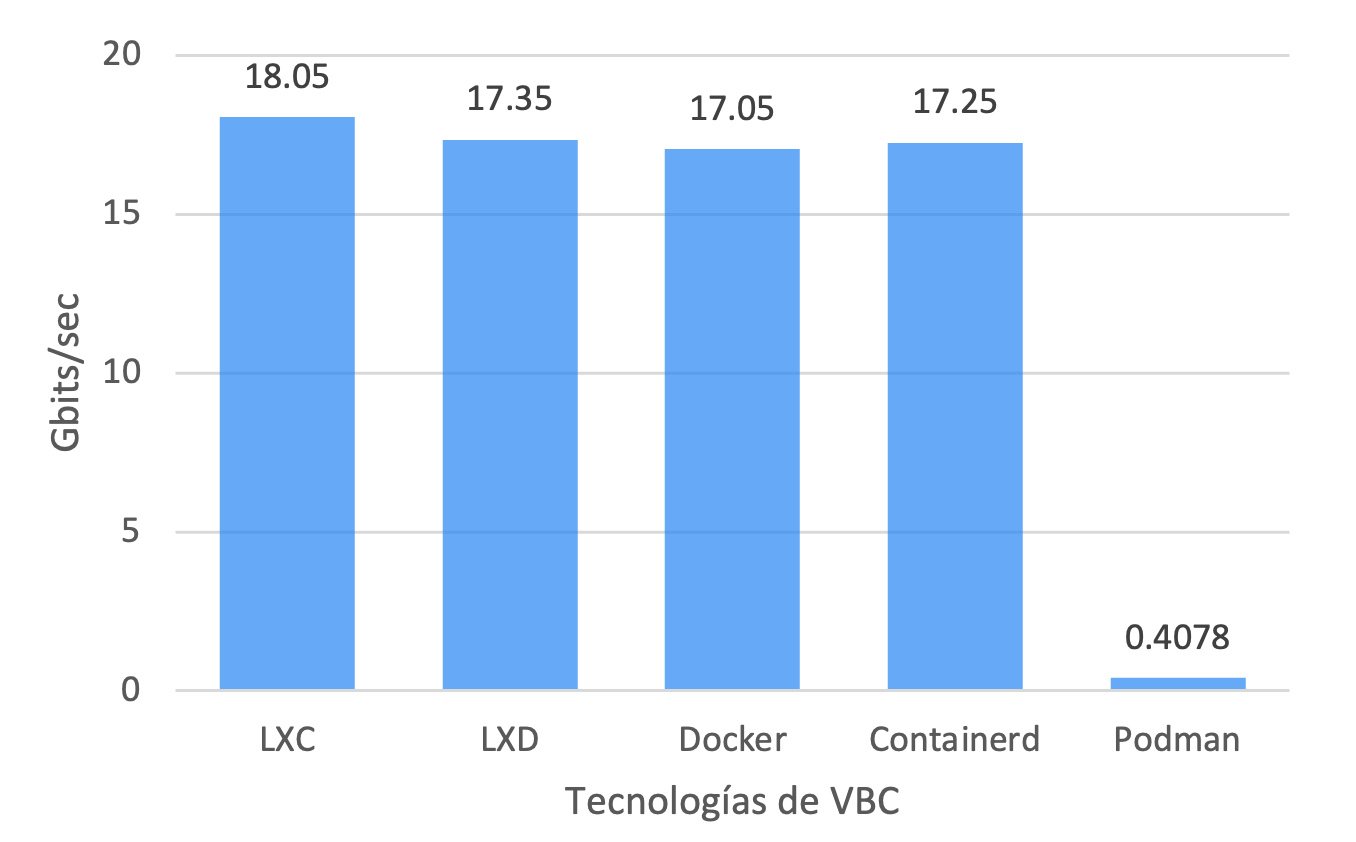
\includegraphics[width=\textwidth] {tablas-images/cp4/THROUGHTPUT.png}
    \caption{Métricas de throughput}\label{fig:tabla-metricas-throughput}
\end{figure}

\section{Análisis de los resultados}

Los resultados obtenidos a partir de las pruebas permiten identificar comportamientos diferenciados entre las tecnologías de contenerización evaluadas. \textbf{Containerd} se posiciona como una de las soluciones más equilibradas, con excelente tiempo de arranque, bajo uso de CPU y buena latencia de disco, lo que lo hace ideal para entornos donde la eficiencia es prioritaria.

\textbf{LXC} mostró consistentemente el menor consumo de recursos y alto rendimiento en red, lo que lo convierte en una opción sólida para sistemas embebidos o despliegues que requieren un uso mínimo de \textit{overhead}. 

Por otro lado, \textbf{Docker} ofreció un rendimiento aceptable, pero con mayores niveles de consumo de CPU y latencia de disco, compensados por su madurez y ecosistema. 

\textbf{LXD}, al estar basado en LXC, heredó parte de sus beneficios, especialmente en uso de red, aunque con un ligero incremento en el tiempo de arranque. 

En contraste, \textbf{Podman}, si bien eficiente en uso de CPU y memoria, presentó resultados considerablemente bajos en el \textit{throughput} de red y alta latencia de disco, lo cual podría limitar su aplicación en cargas sensibles a E/S o comunicación intensiva.

\vspace{0.5em}

\noindent En resumen, la elección de la tecnología de contenerización debe considerar el caso de uso específico: \textbf{Containerd} y \textbf{LXC} sobresalen en eficiencia general; \textbf{Docker} y \textbf{LXD} ofrecen robustez y facilidad de integración; mientras que \textbf{Podman} puede ser más adecuado para entornos que prioricen la seguridad y compatibilidad con el modelo sin \textit{daemon}, siempre que el rendimiento de red o disco no sea crítico.

\ChapterImageStar[cap:dar]{Análisis de Decisiones y Resolución}{./images/fondo.png}\label{cap:dar}
\mbox{}\\
\section{Metodología de evaluación}

La metodología de evaluación que se aplicó para la elección de la tecnología de Virtualización Basada en Contenedores (VBC) fue DAR (Decision, analysis and resolution) de CMMI \citep{CMMIInstitute2010}. Esta metodología permitió evaluar las necesidades del grupo GRID a través de un proceso estructurado que consideró múltiples alternativas, criterios de evaluación bien definidos y un análisis comparativo. En este caso, se identificaron y analizaron diversas tecnologías VBC —como Docker, Podman, LXC o Kata Containers— aplicando criterios como el tipo de licencia, la compatibilidad con herramientas de orquestación, el rendimiento entre otros. Mediante el uso de matrices DOFA, se logró visualizar las fortalezas y debilidades de cada opción, facilitando una selección alineada con los objetivos estratégicos del sistema. Así, el uso de DAR no solo aportó transparencia al proceso, sino también trazabilidad y justificación técnica frente a una decisión para la arquitectura de infraestructura basada en contenedores.

El proceso de evaluación quedó registrado en un vídeo explicativo disponible en \href{https://youtu.be/xOmuQs2RX2c}{link}.

\section{Resultados de la evaluación}

\begin{table}[H]
    \centering
    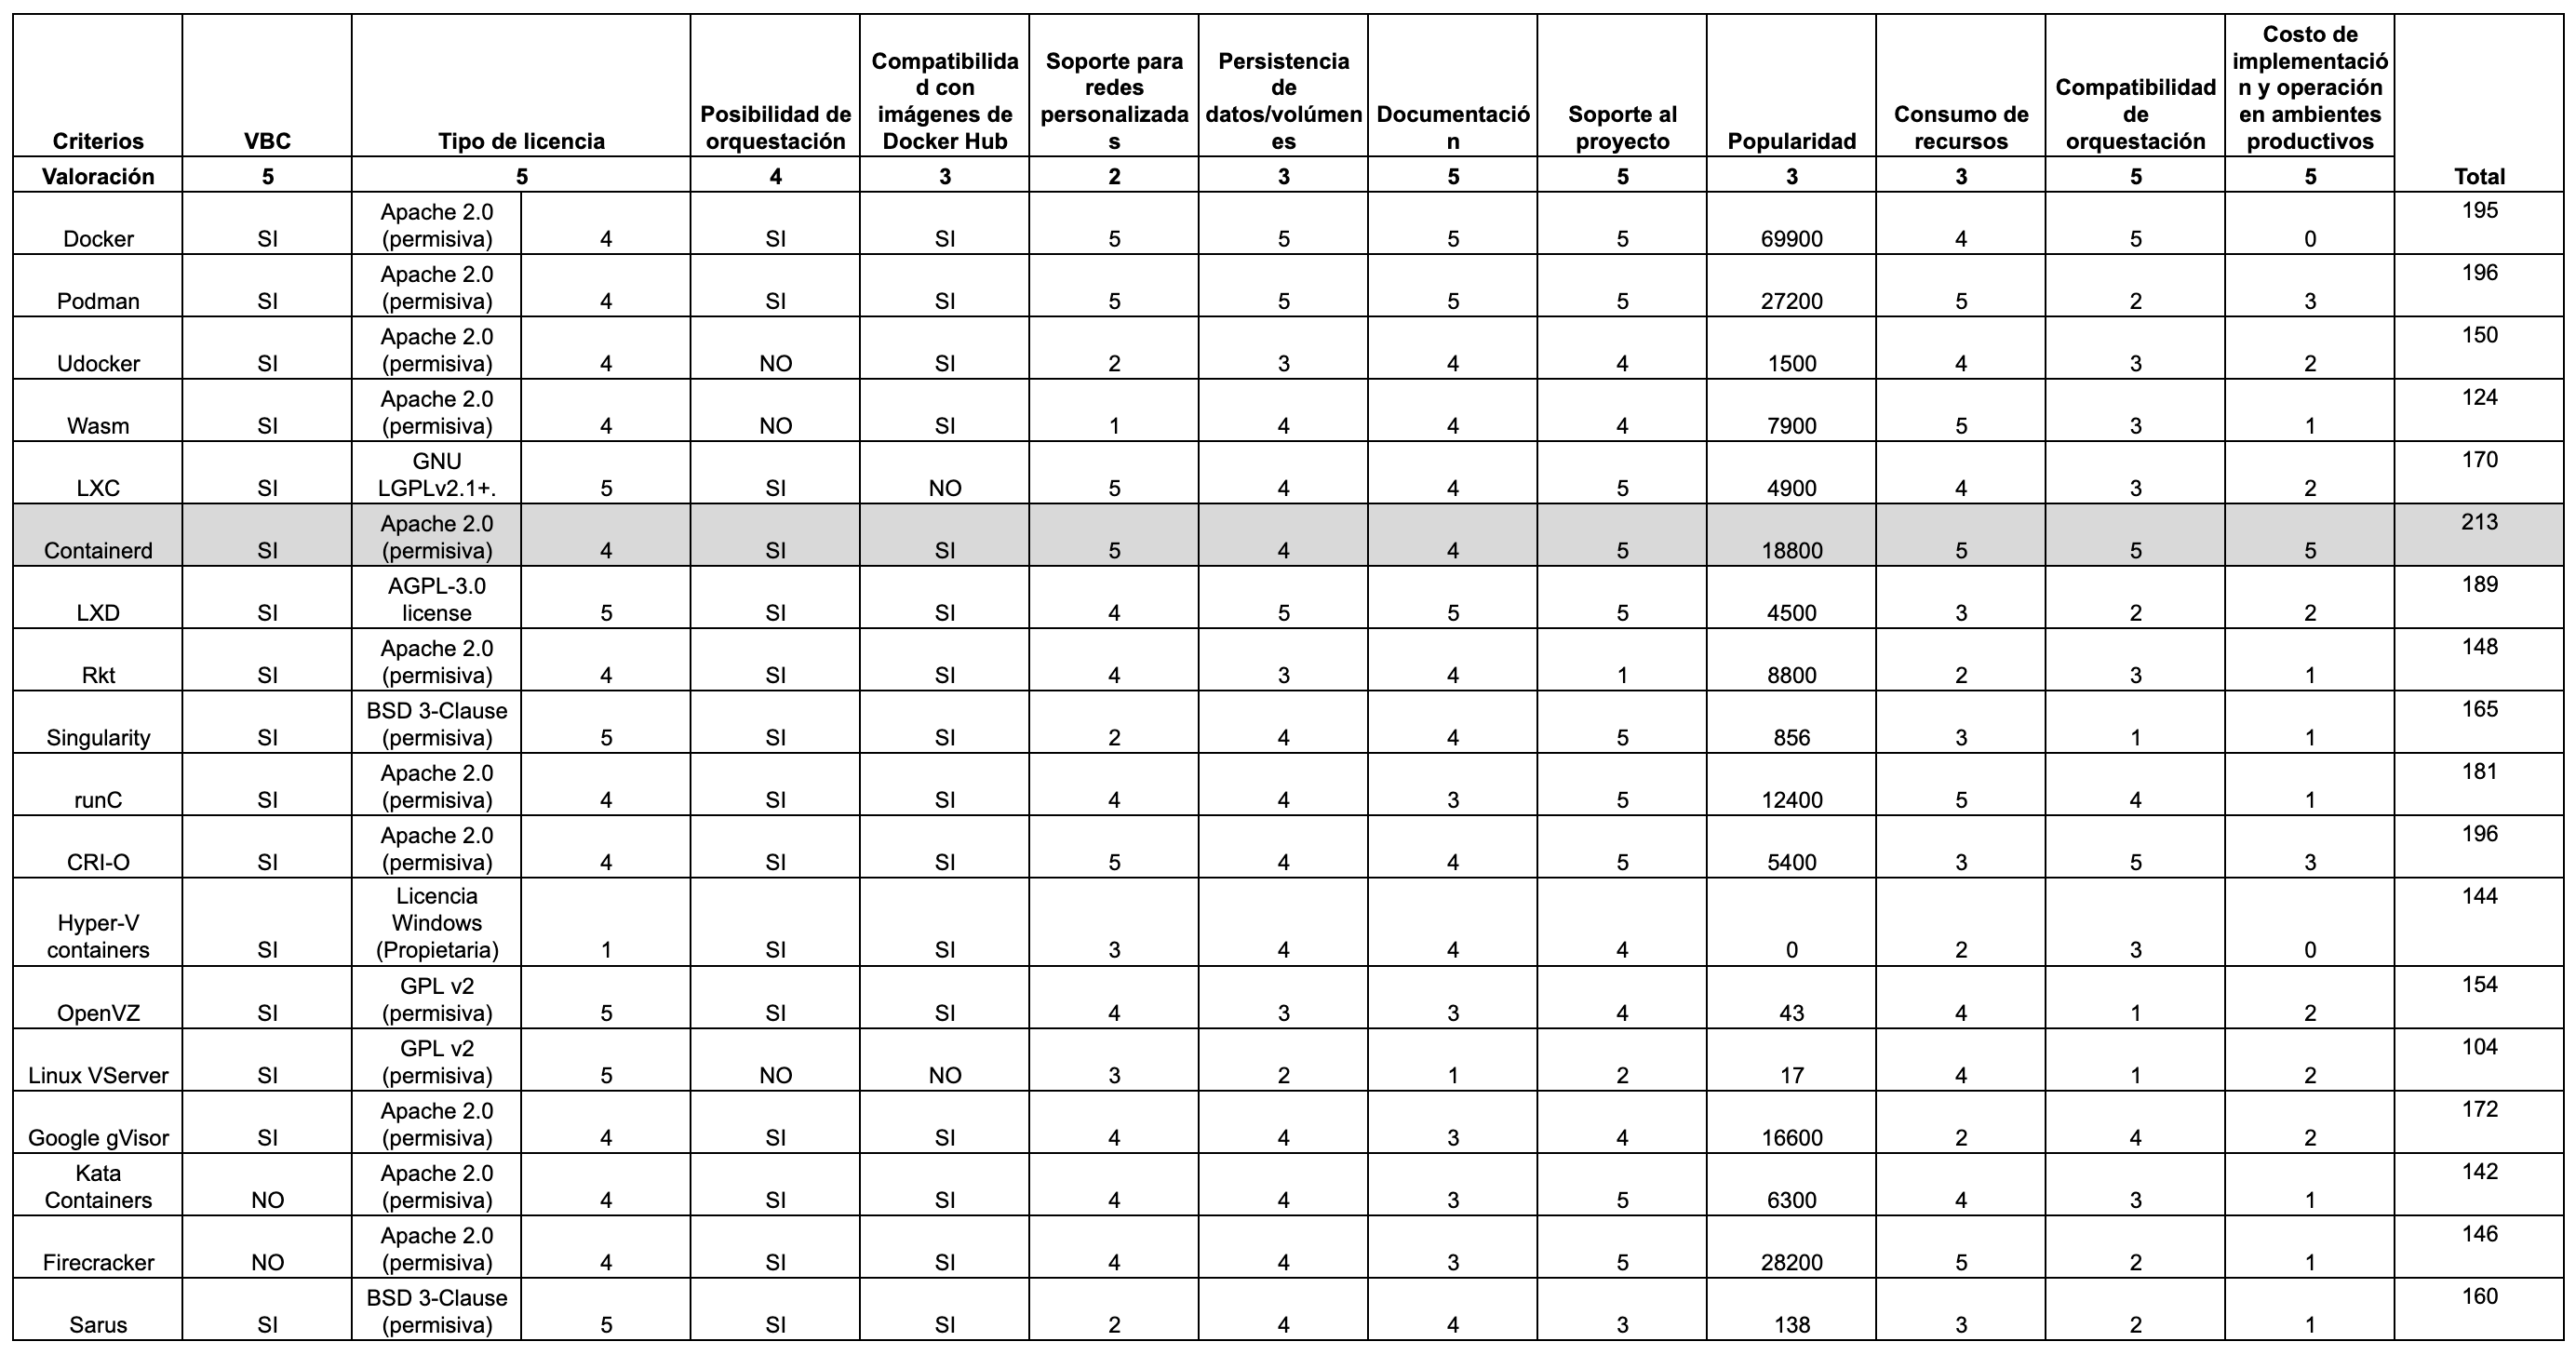
\includegraphics[width=\textwidth] {tablas-images/cp5/DAR.png}
    \caption{Análisis de Decisiones y Resolución (DAR) aplicado a la selección de VBC}\label{tab:tabla-dar}
\end{table}

\section{Criterios de evaluación}

\subsection{VBC (¿Es una tecnología basada en contenedores?)}
Este criterio define si la tecnología analizada entra dentro de la categoría de virtualización basada en contenedores, lo cual es el punto de partida para que pueda ser considerada en el análisis. Se evalúa como Sí (SI) o No (NO).

\subsection{Tipo de licencia}
Se analiza el tipo de licencia bajo la cual se distribuye la tecnología, ya que esto afecta su adopción en proyectos académicos o comerciales. Las licencias permisivas (como Apache 2.0 o BSD) permiten mayor libertad de uso y modificación, mientras que licencias restrictivas (como AGPL o licencias propietarias) imponen ciertas limitaciones legales o técnicas.

\subsection{Posibilidad de orquestación}
Se refiere a la capacidad de la tecnología para integrarse con herramientas de orquestación como Kubernetes, Docker Swarm o Nomad, lo cual es clave para la gestión automatizada de contenedores a gran escala. Una mayor puntuación indica mejor compatibilidad y soporte para estas herramientas.

\subsection{Compatibilidad con imágenes de Docker Hub}
Evalúa si la tecnología puede ejecutar imágenes obtenidas directamente desde Docker Hub, el repositorio más utilizado para contenedores. Esto facilita la reutilización de contenedores existentes y la integración con flujos de trabajo ya establecidos.

\subsection{Soporte para redes personalizadas}
Determina si la tecnología permite la creación y gestión de redes personalizadas entre contenedores. Este aspecto es fundamental en arquitecturas distribuidas, donde la comunicación entre servicios debe configurarse de forma segura.

\subsection{Persistencia de datos / volúmenes}
Analiza si la solución permite la persistencia de datos, es decir, que los datos generados dentro de un contenedor puedan mantenerse incluso después de reiniciarlo o eliminarlo. Esto se logra mediante el uso de volúmenes o sistemas de almacenamiento externos.

\subsection{Documentación}
Se valora la calidad, profundidad y accesibilidad de la documentación oficial. Una buena documentación facilita el aprendizaje, la resolución de problemas y la implementación efectiva de la tecnología.

\subsection{Soporte al proyecto}
Considera el respaldo que tiene la tecnología por parte de la comunidad, empresas o fundaciones (como CNCF o Red Hat). Esto incluye mantenimiento activo, actualizaciones regulares, y foros o canales de ayuda disponibles.

\subsection{Popularidad}
Este criterio mide la adopción y visibilidad de la tecnología, lo cual puede reflejar su madurez, confianza del mercado y disponibilidad de talento capacitado. Se puede estimar por métricas como el número de estrellas en GitHub.

\subsection{Consumo de recursos}
Evalúa el nivel de consumo de recursos respecto al uso de CPU, memoria y almacenamiento. Se valora según lo que mencionan las organizaciones en este aspecto.

\subsection{Compatibilidad de orquestación}
Difiere levemente del punto 4.3, ya que aquí se mide qué tan bien se integra con los orquestadores, considerando estabilidad, plugins nativos y experiencia de uso. Un puntaje alto indica integración fluida y confiable.

\subsection{Costo de implementación y operación en ambientes productivos}
Este criterio analiza los costos asociados a poner en marcha la tecnología en un entorno real. Incluye licencias, infraestructura, tiempo de configuración y mantenimiento. Una puntuación alta significa bajo costo o costo nulo, lo cual es ideal para instituciones académicas o proyectos con presupuesto limitado.

\section{Tecnología VBC ganadora}

Del análisis comparativo realizado, Containerd se posiciona como la tecnología de virtualización basada en contenedores con mejor desempeño general. Destaca por su alta compatibilidad con Docker Hub, soporte para redes y volúmenes, excelente integración con orquestadores como Kubernetes, y una licencia permisiva que facilita su adopción. Además, cuenta con una sólida documentación y un respaldo activo de la comunidad. Estas características hacen de Containerd la opción adecuada para ser implementada en ambientes productivos del grupo de investigación GRID, combinando los diferentes criterios definidos desde el grupo de investigación.

\section{Análisis DAR del motor de Kubernetes}

\begin{table}[H]
    \centering
    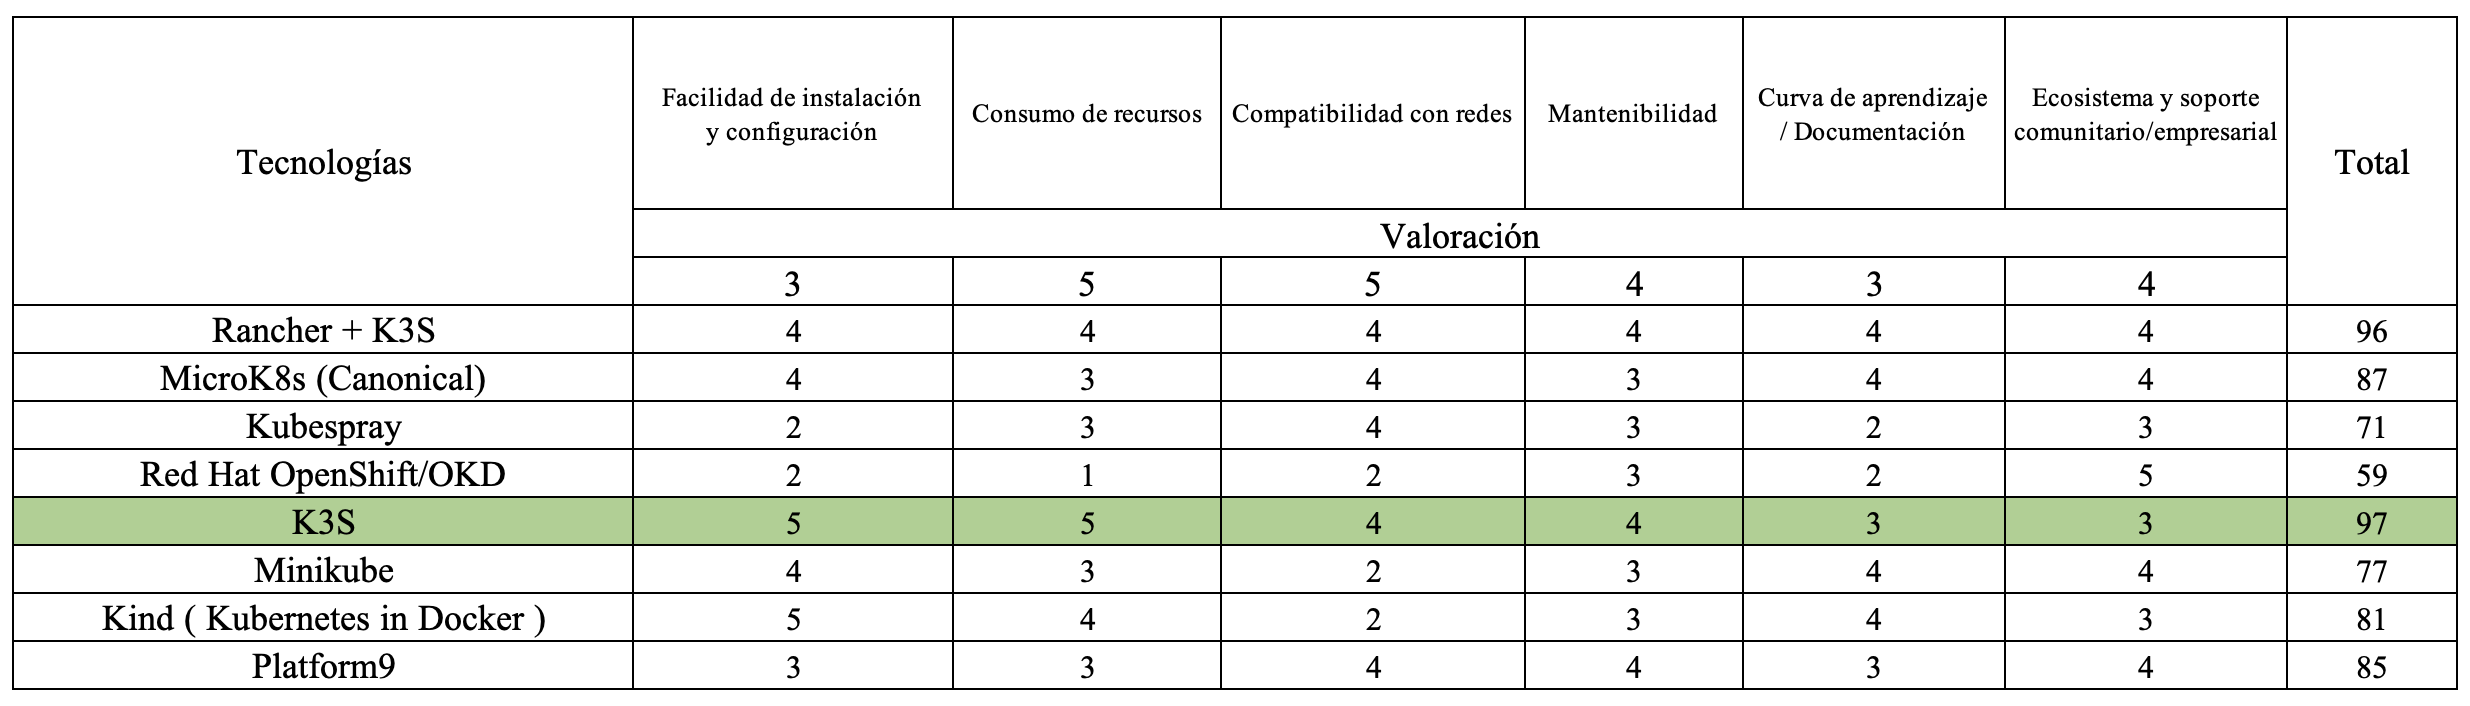
\includegraphics[width=\textwidth] {tablas-images/cp5/dar-k8s.png}
    \caption{Análisis de Decisiones y Resolución aplicado a la selección del motor de Kubernetes}\label{tab:tabla-dar}
\end{table}
\ChapterImageStar[cap:disenio]{Diseño de la solución}{./images/fondo.png}\label{cap:disenio}
\mbox{}\\
\section{Modelado del sistema en Archimate}

\subsection{Vista de negocio}
\begin{figure}[H]
    \centering
    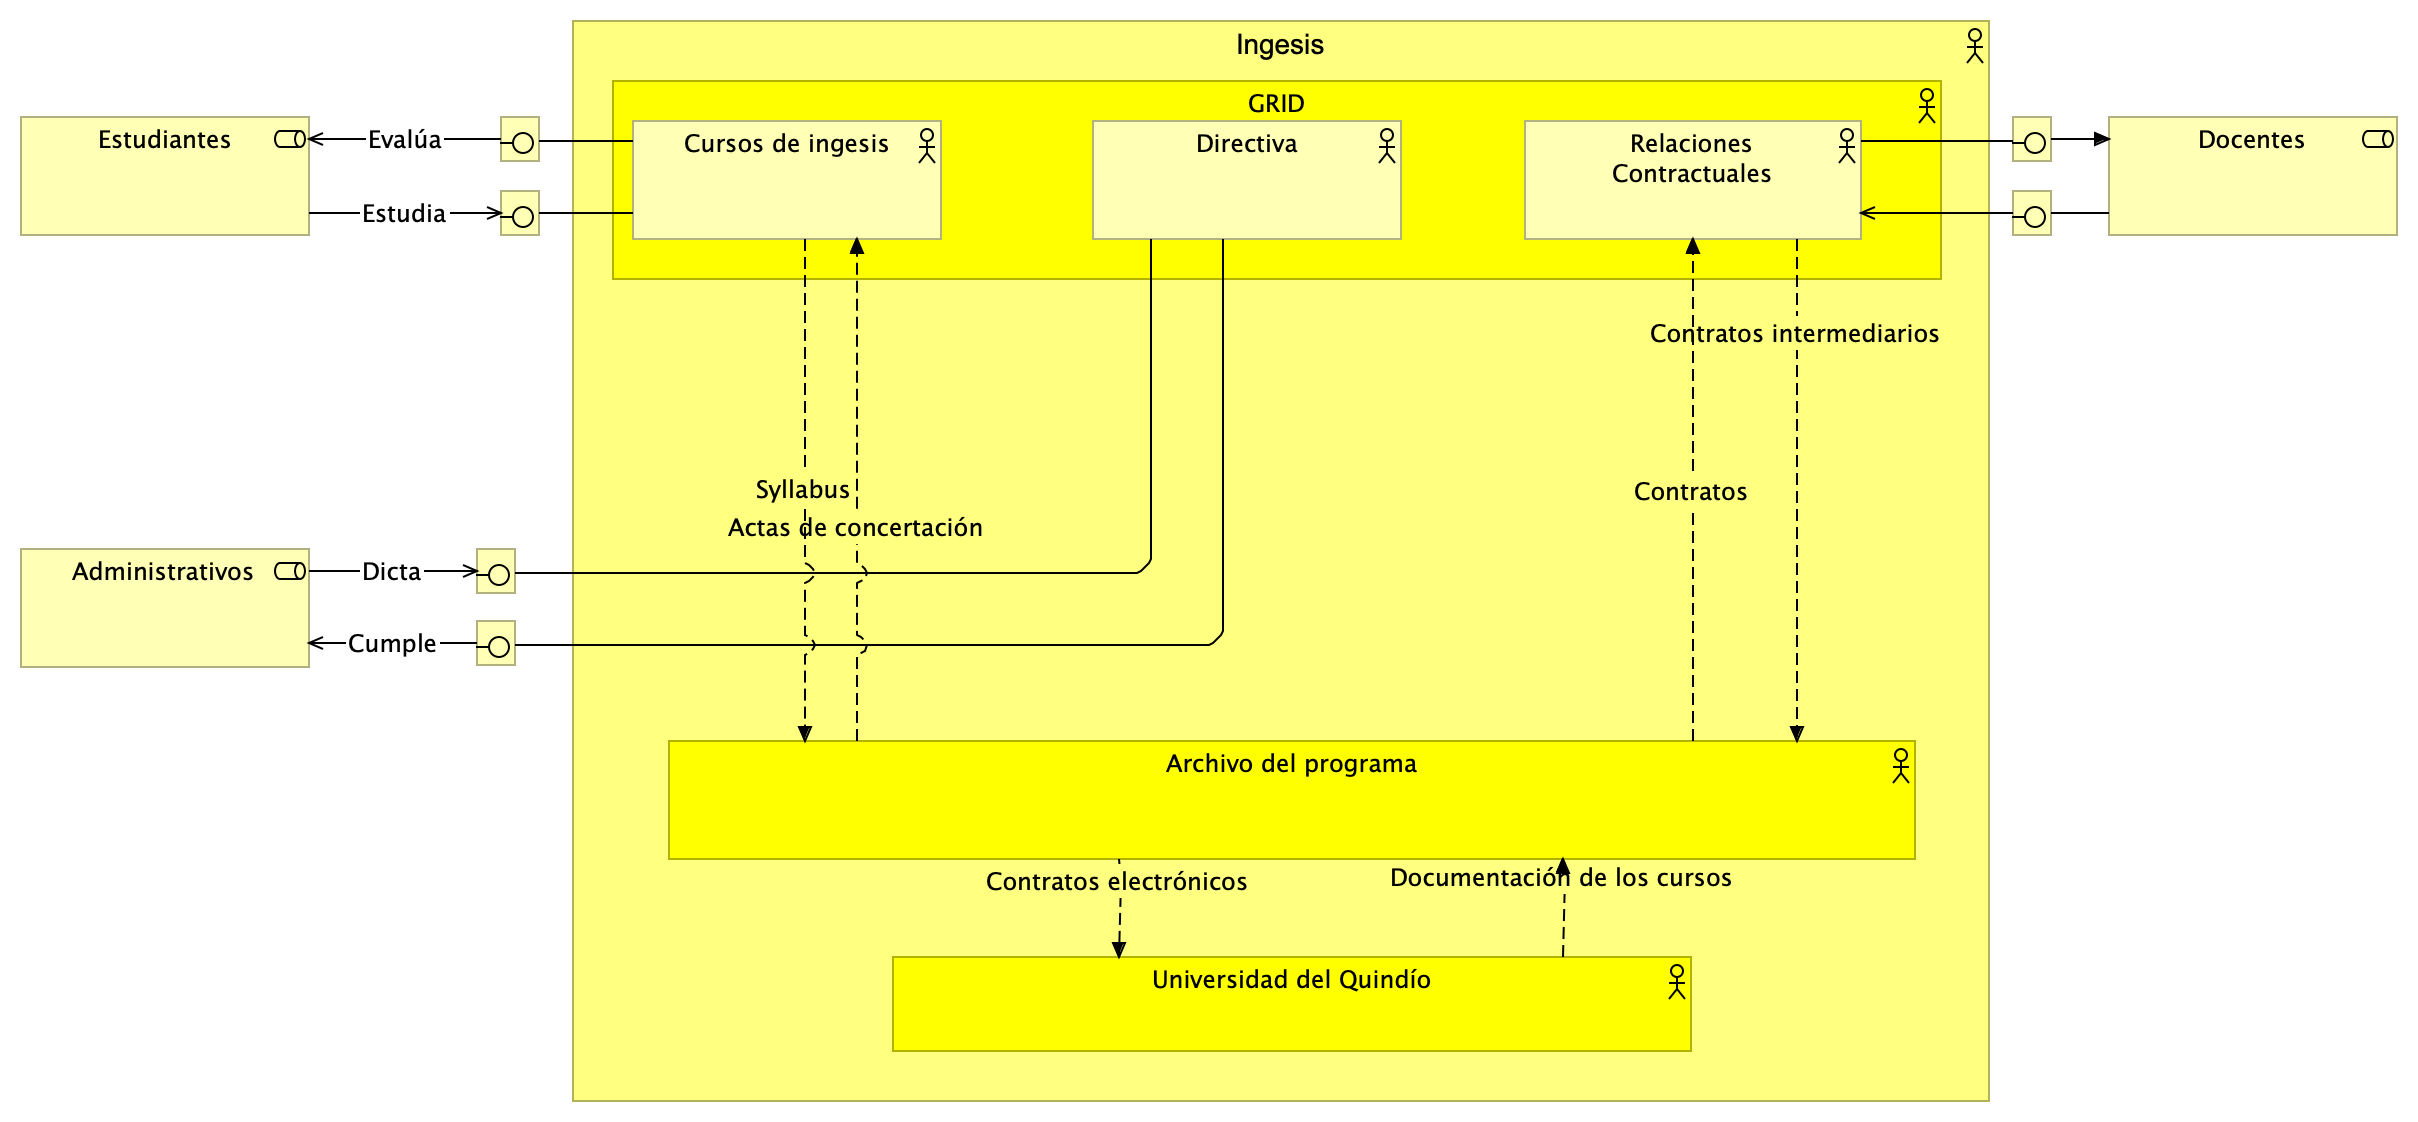
\includegraphics[width=\textwidth]{tablas-images/cp6/Actor-Cooperation-view.png}
    \caption{Vista de Cooperación de Actores}
\end{figure}
\begin{figure}[H]
    \centering
    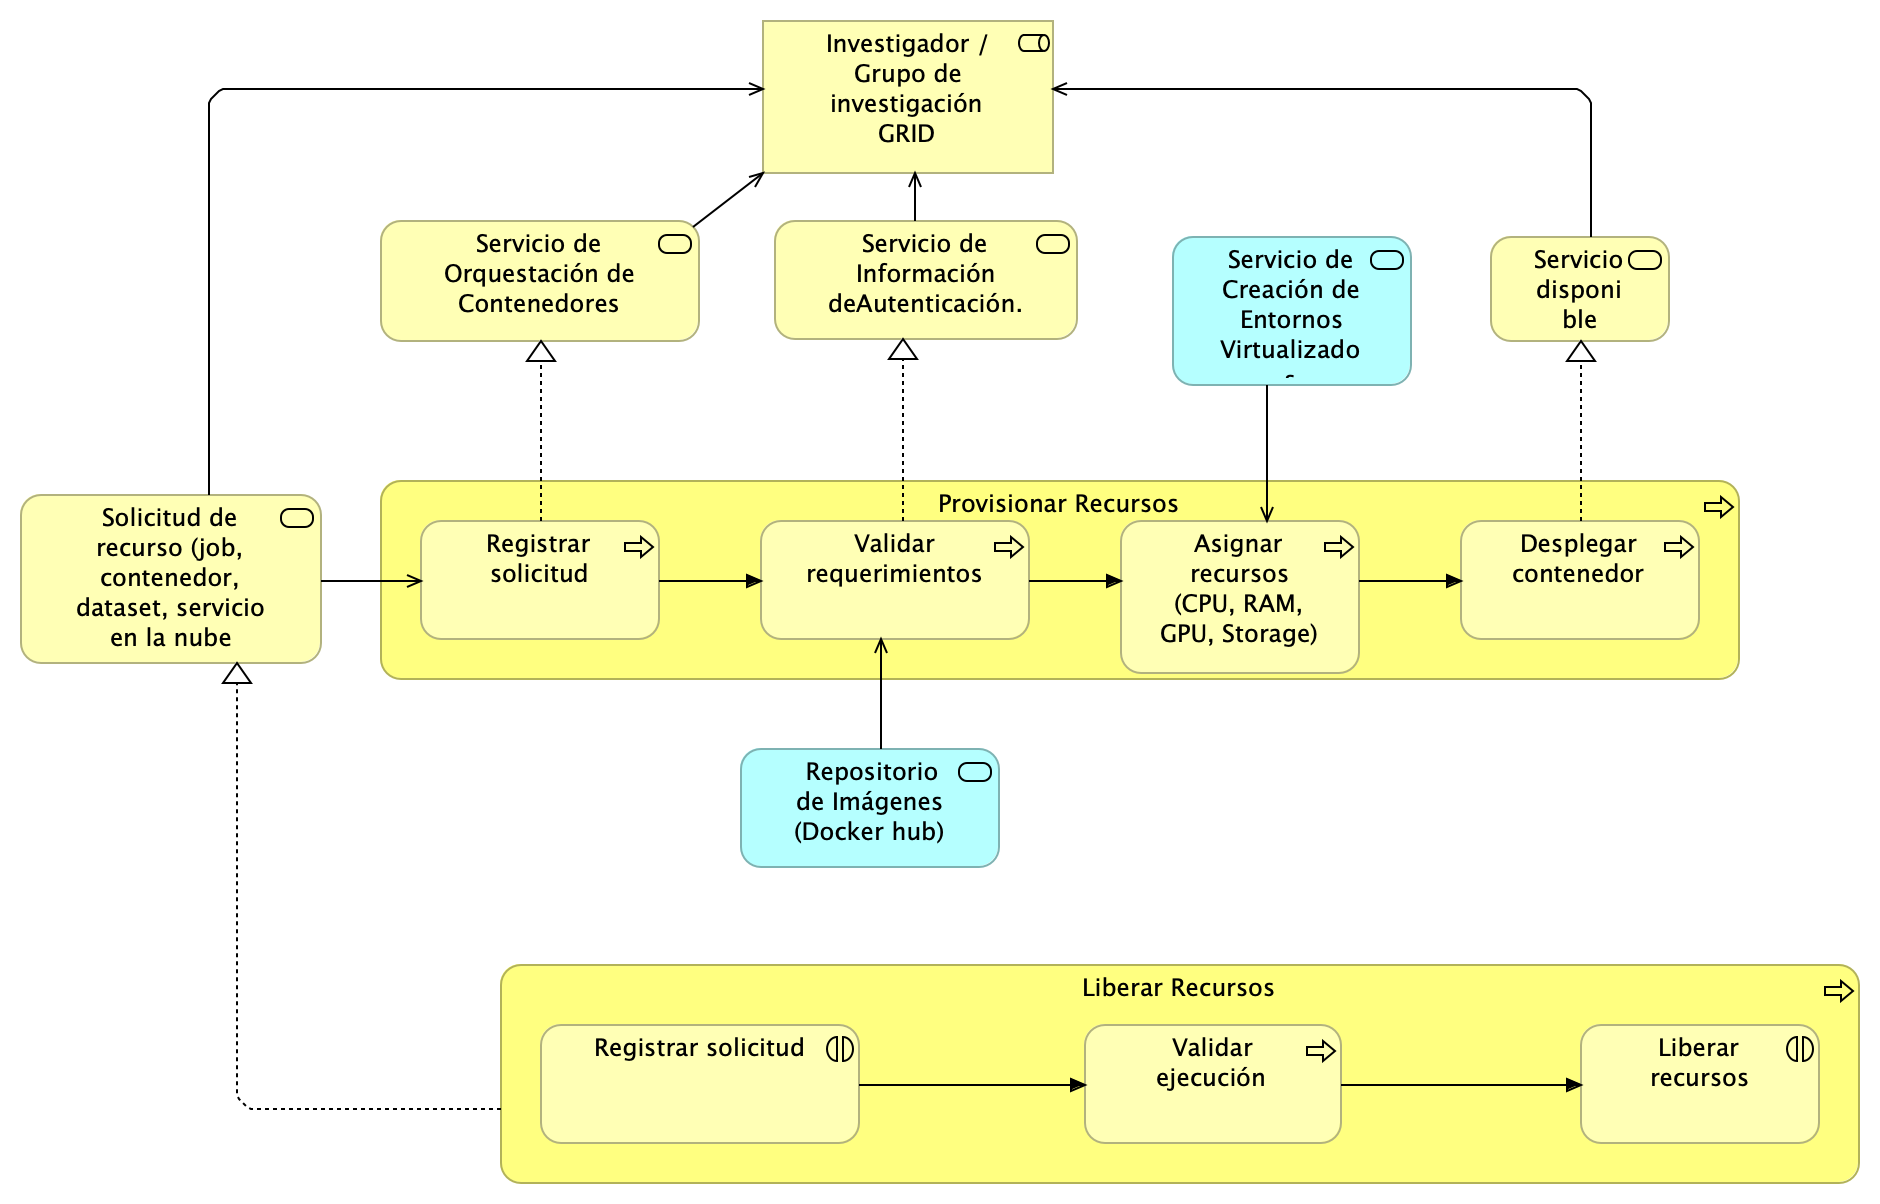
\includegraphics[width=\textwidth]{tablas-images/cp6/Business-Cooperation-View.png}
    \caption{Vista de Cooperación de Negocio}
\end{figure}
\begin{figure}[H]
    \centering
    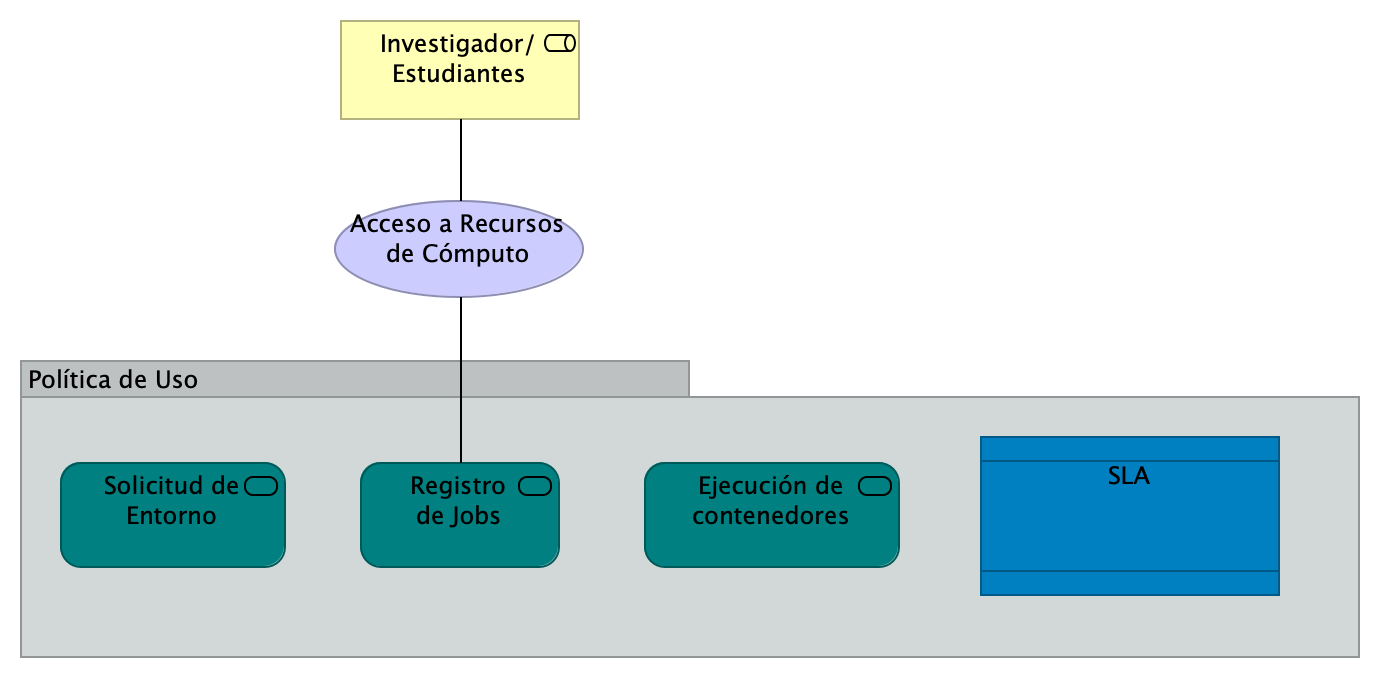
\includegraphics[width=\textwidth]{tablas-images/cp6/Business-Product-View.png}
    \caption{Vista de Producto de Negocio}
\end{figure}
\begin{figure}[H]
    \centering
    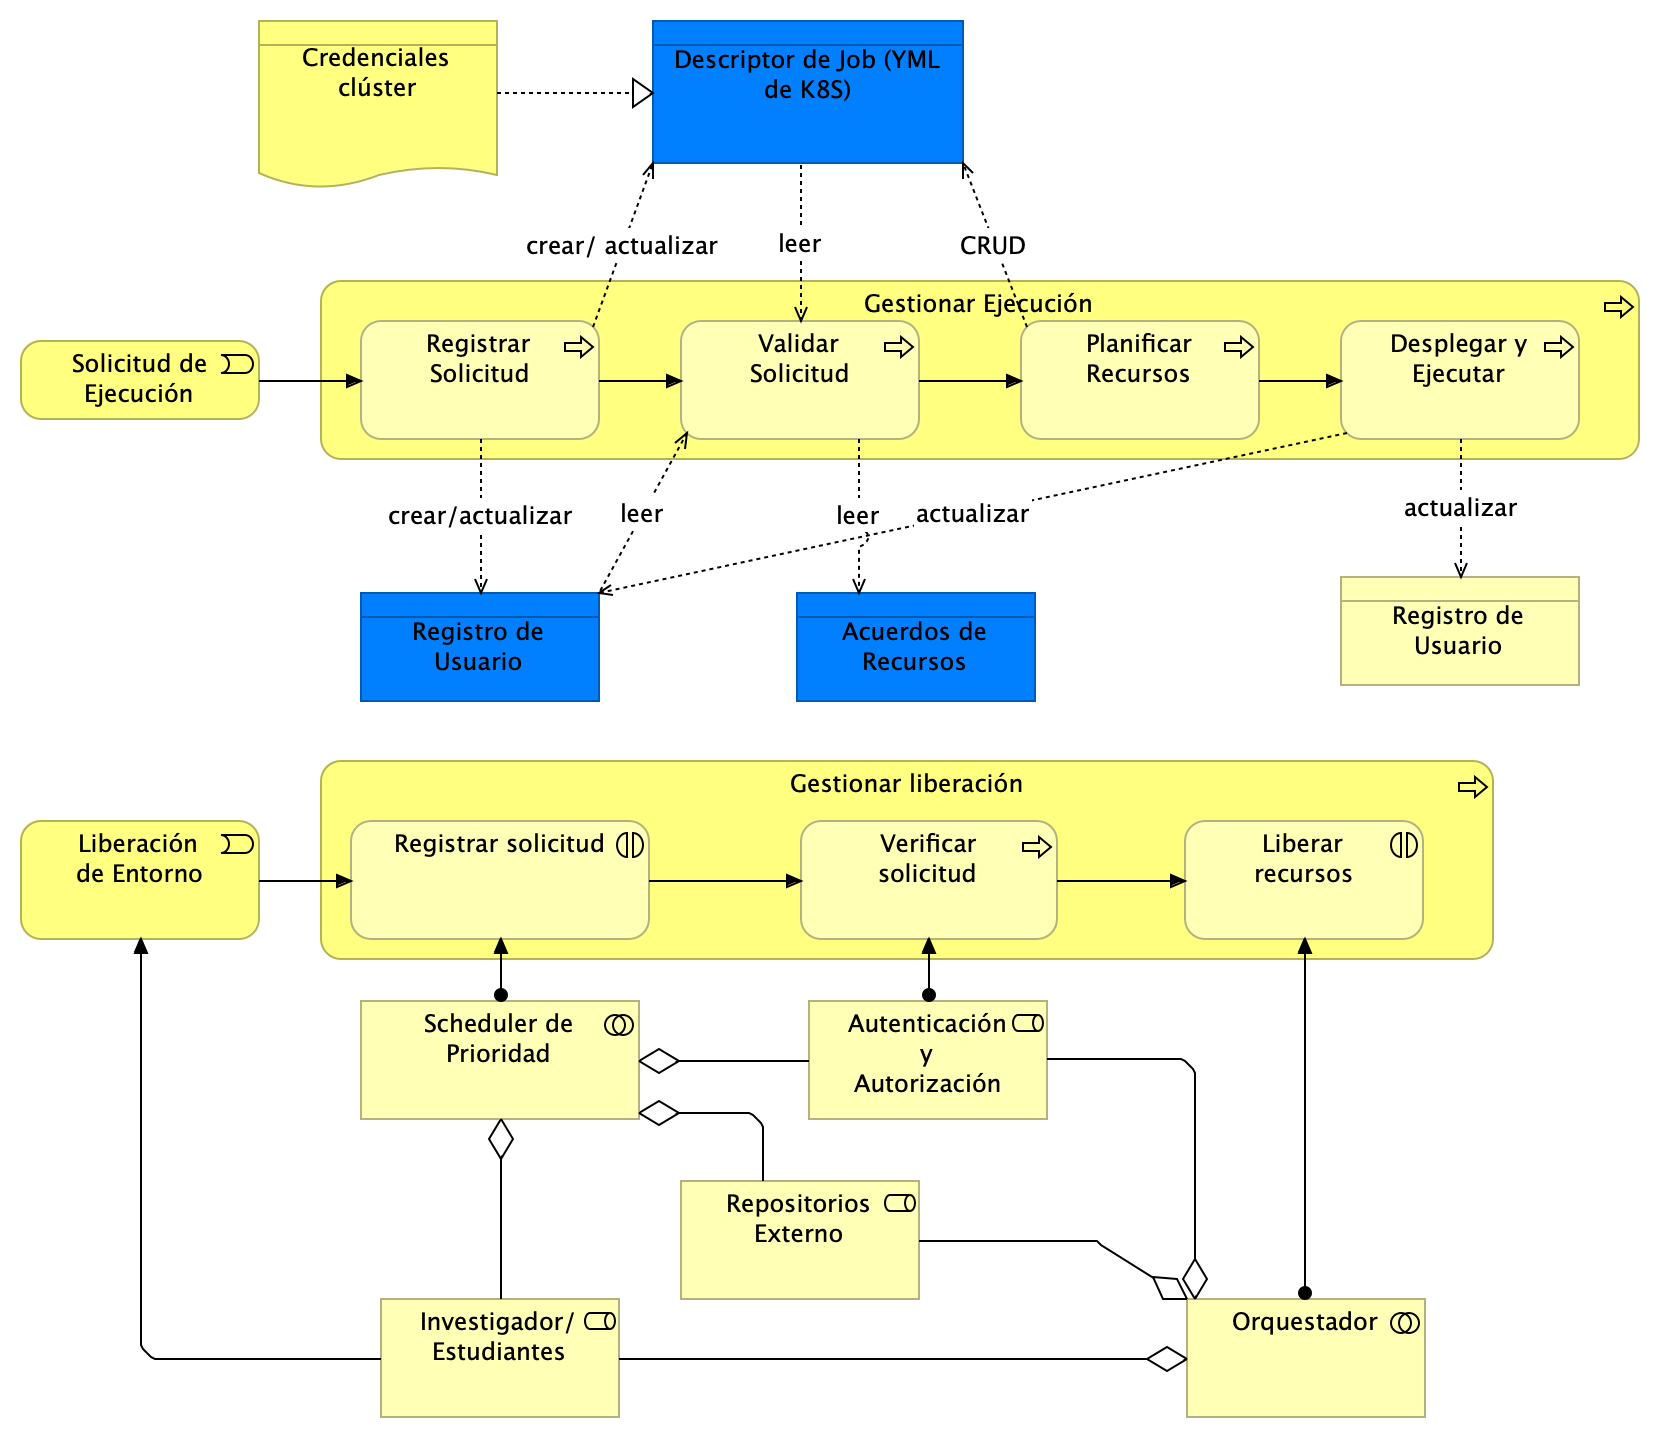
\includegraphics[width=\textwidth]{tablas-images/cp6/Business-Process-View.png}
    \caption{Vista de Proceso de Negocio}
\end{figure}
\begin{figure}[H]
    \centering
    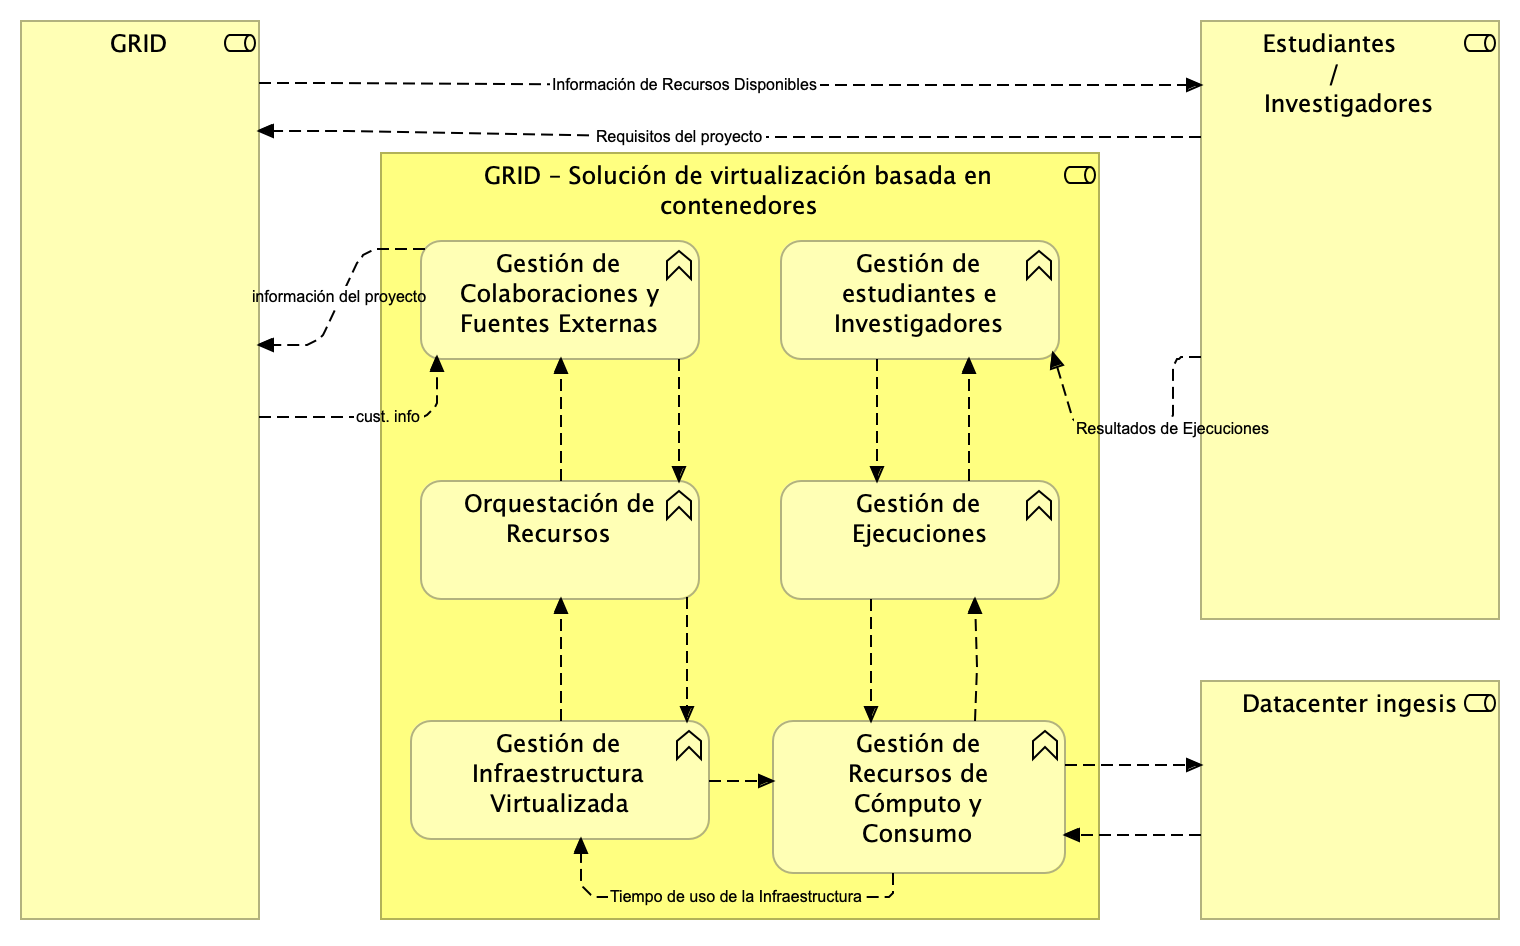
\includegraphics[width=\textwidth]{tablas-images/cp6/Business-Function-View.png}
    \caption{Vista de Función de Negocio}
\end{figure}



\subsection{Vista de aplicación}
\begin{figure}[H]
    \centering
    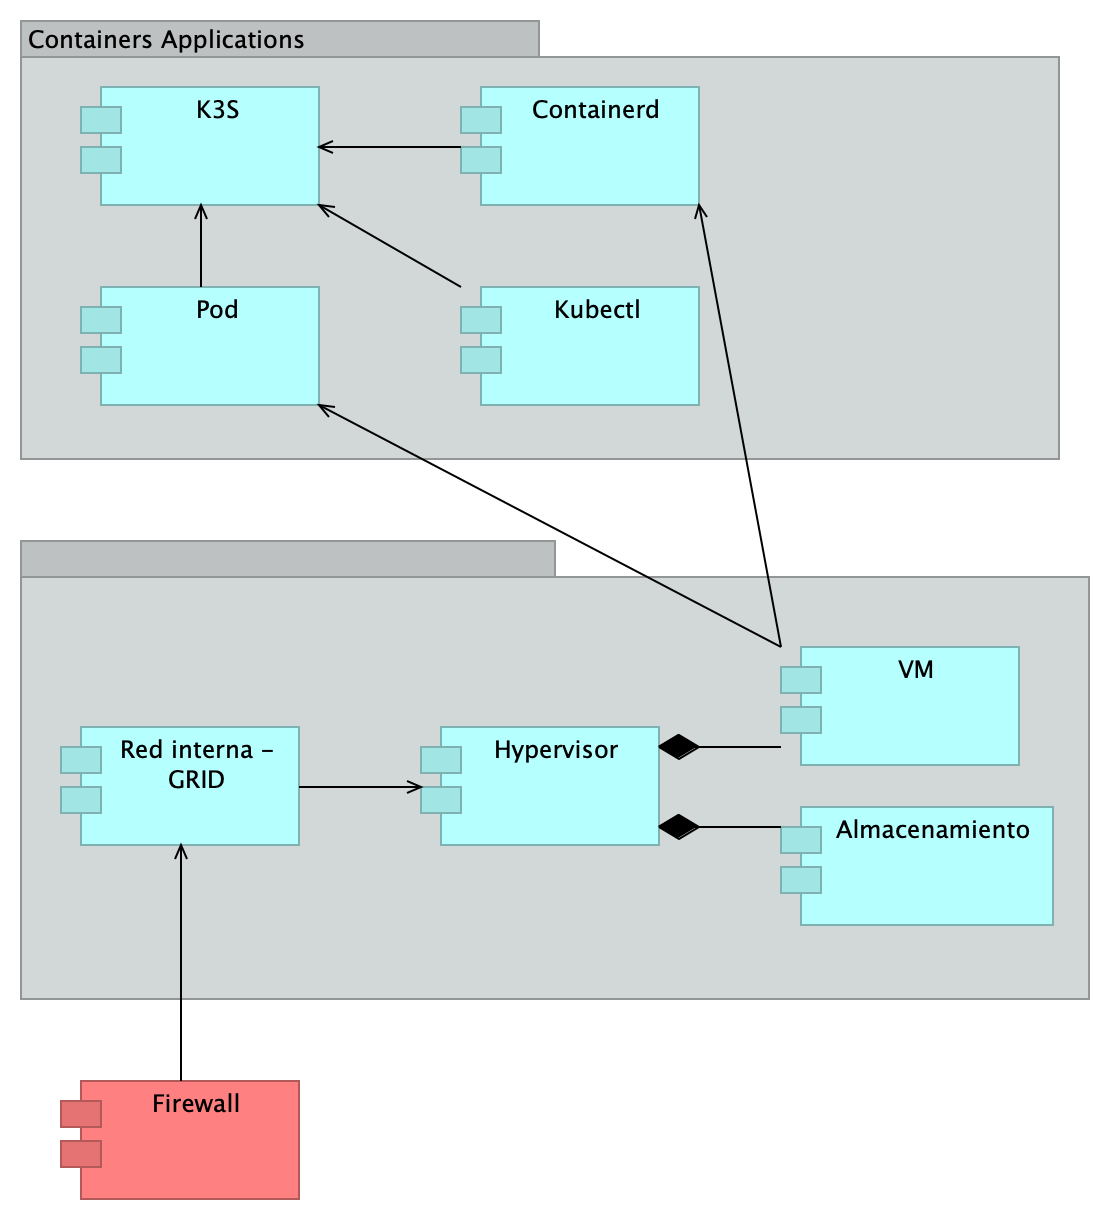
\includegraphics[width=\textwidth]{tablas-images/cp6/Application-Cooperation-View.png}
    \caption{Vista de Cooperación de Aplicaciones}
\end{figure}
\begin{figure}[H]
    \centering
    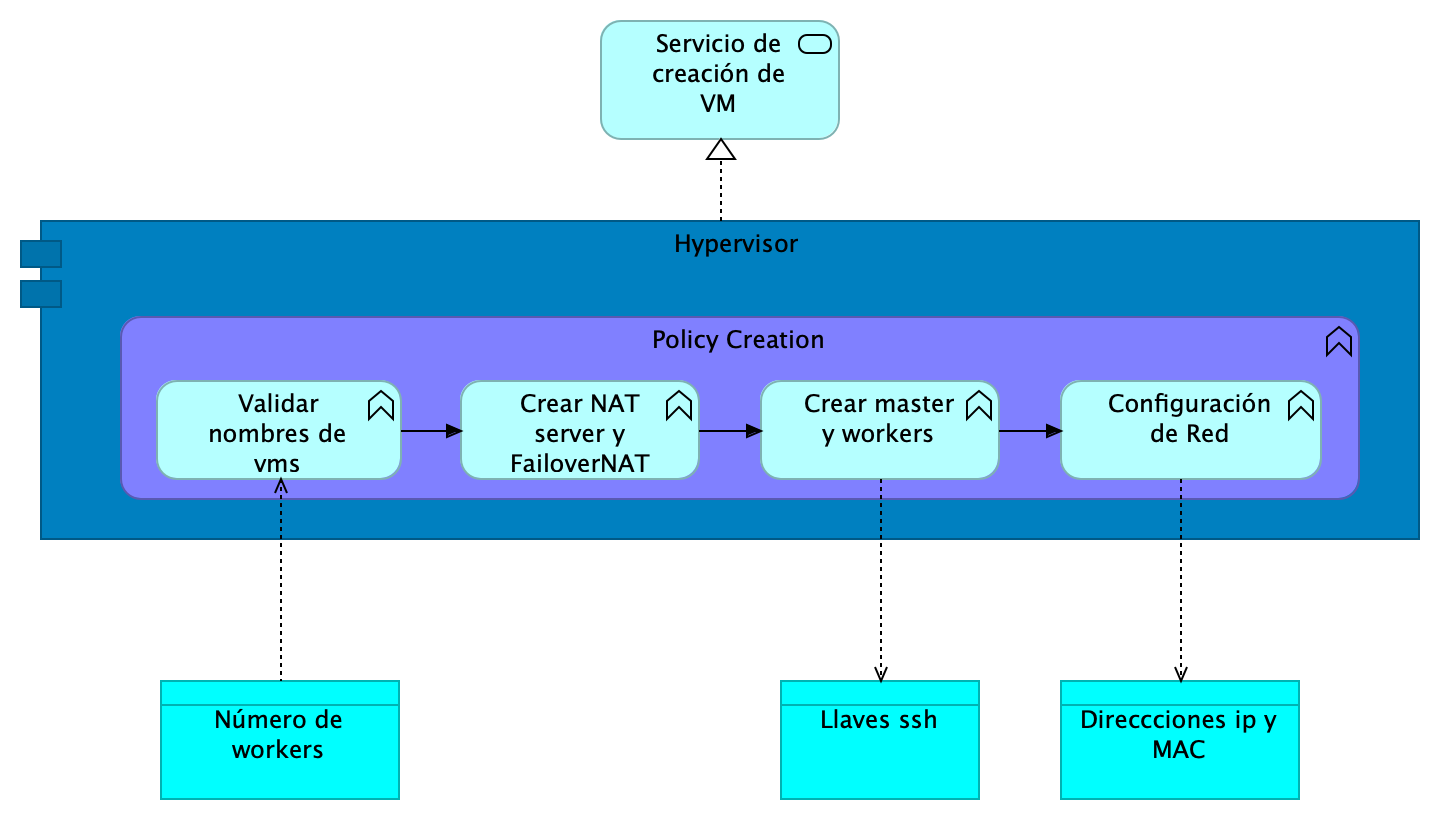
\includegraphics[width=\textwidth]{tablas-images/cp6/Application-Behaviour-view.png}
    \caption{Vista de Comportamiento de Aplicaciones}
\end{figure}
\begin{figure}[H]
    \centering
    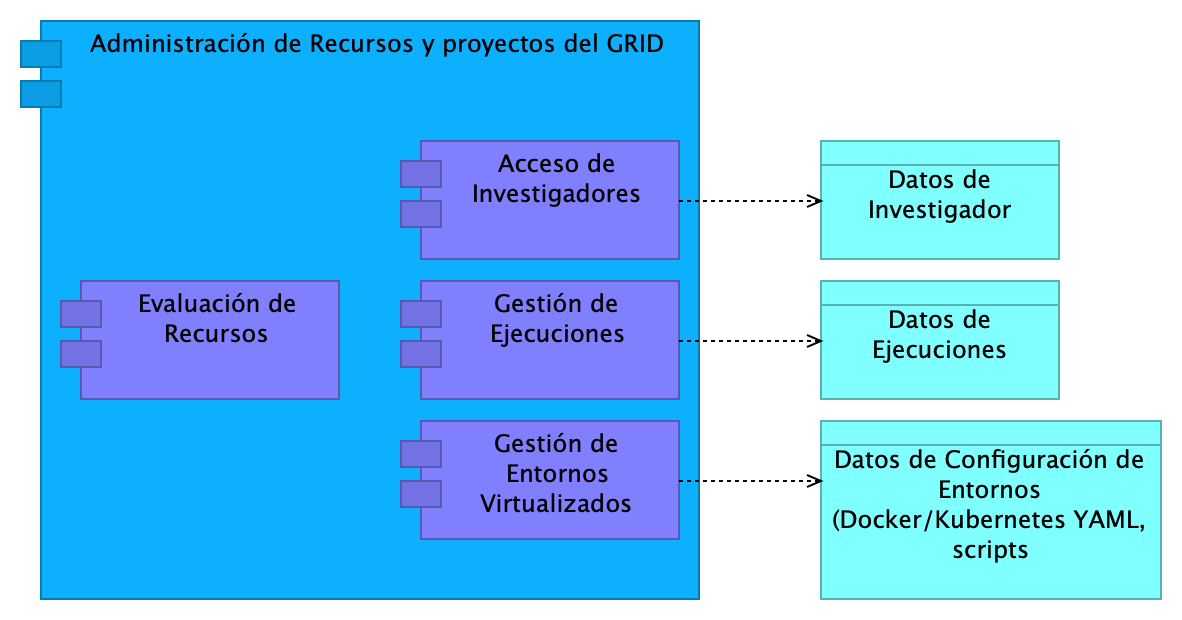
\includegraphics[width=\textwidth]{tablas-images/cp6/Application-Structure-View.png}
    \caption{Vista de Estructura de Aplicaciones}
\end{figure}

\subsection{Vista de tecnología}
\begin{figure}[H]
    \centering
    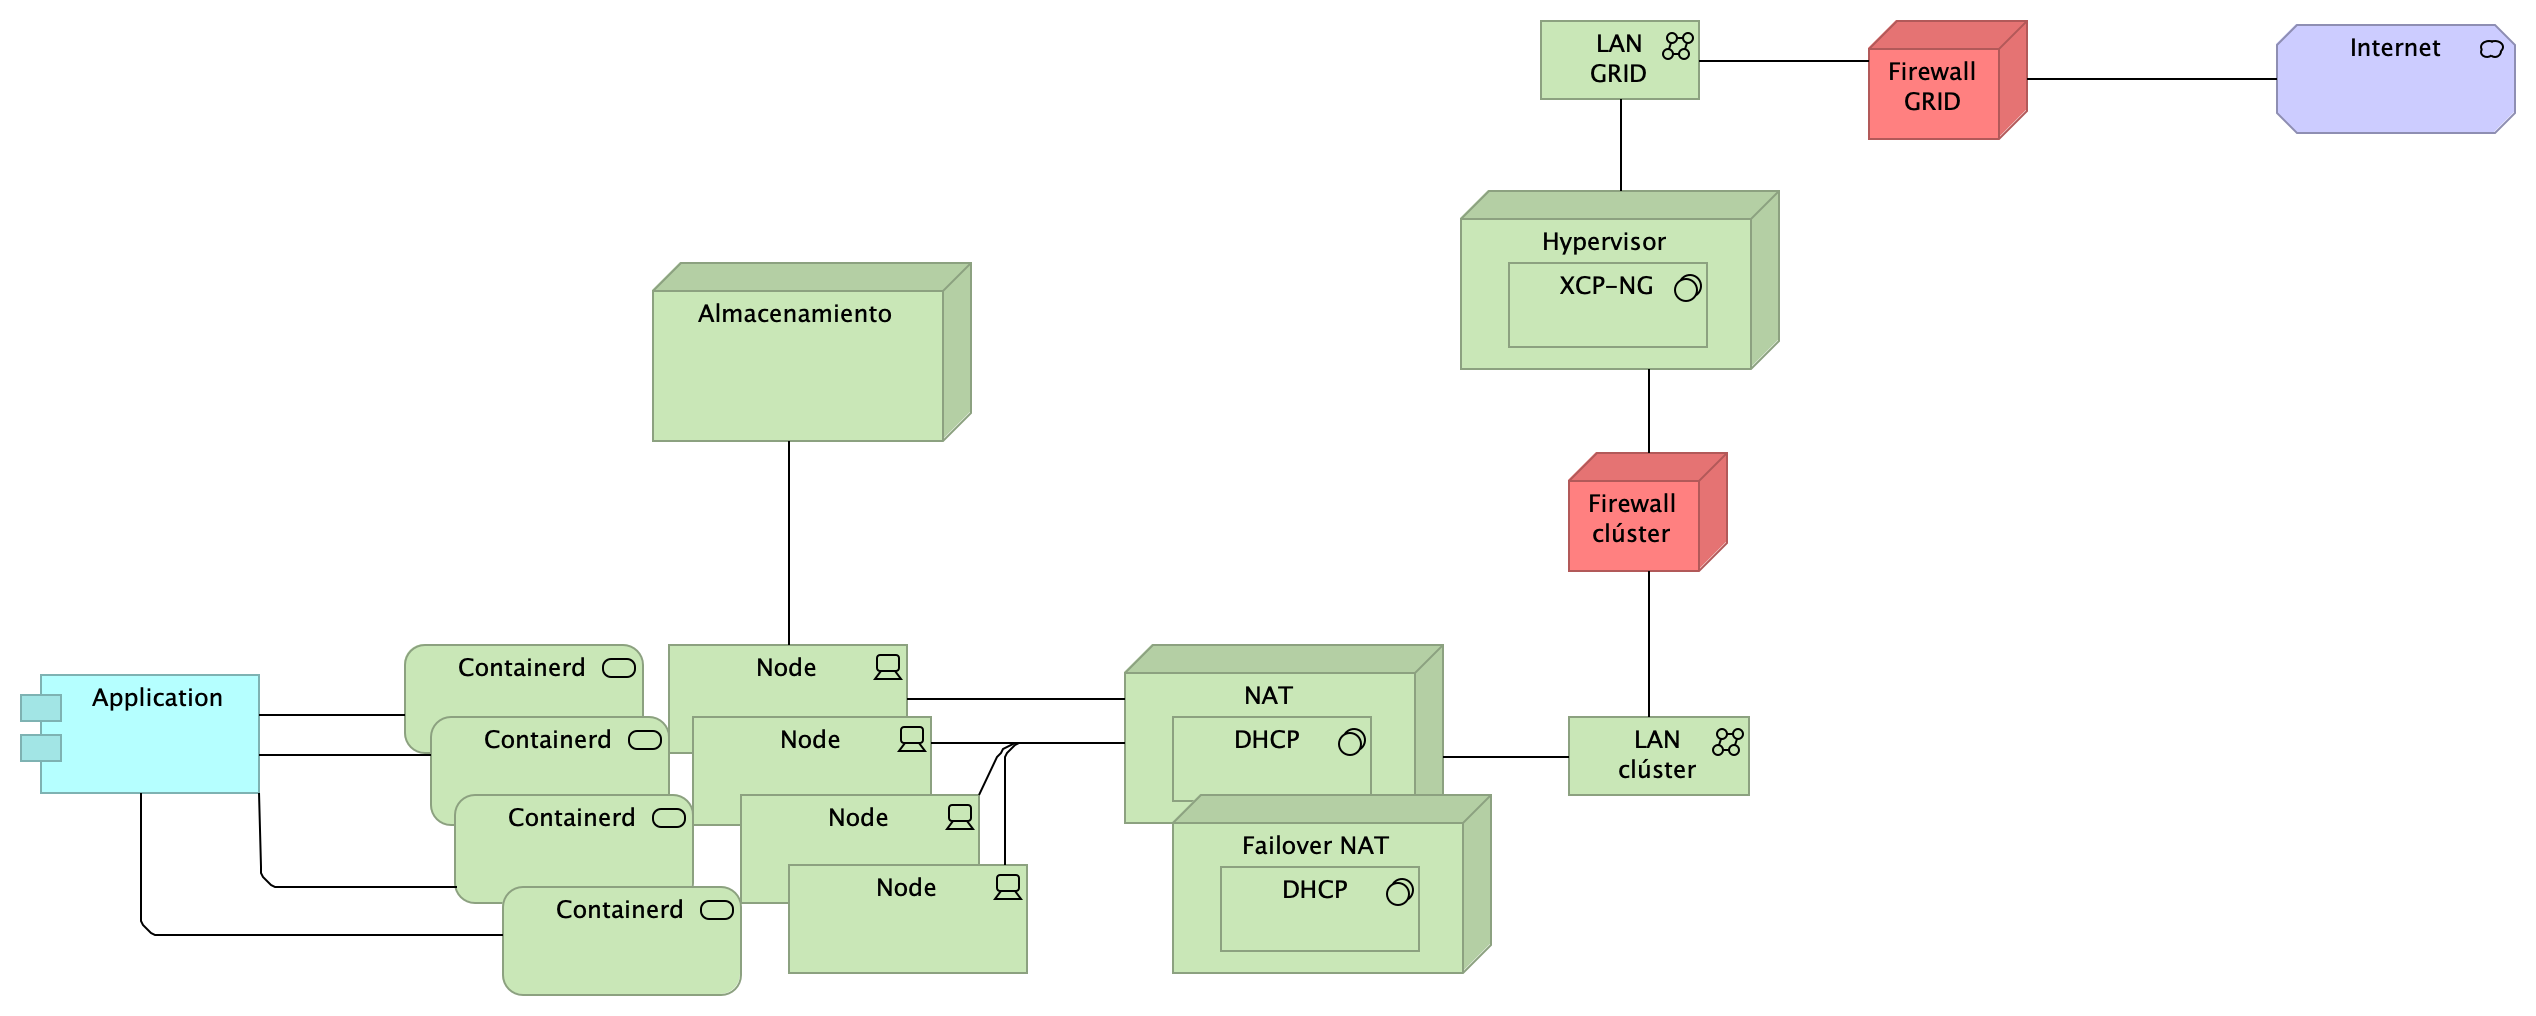
\includegraphics[width=\textwidth]{tablas-images/cp6/Implementation-and-Installation-View.png}
    \caption{Vista de Implementación e Instalación}
\end{figure}
\begin{figure}[H]
    \centering
    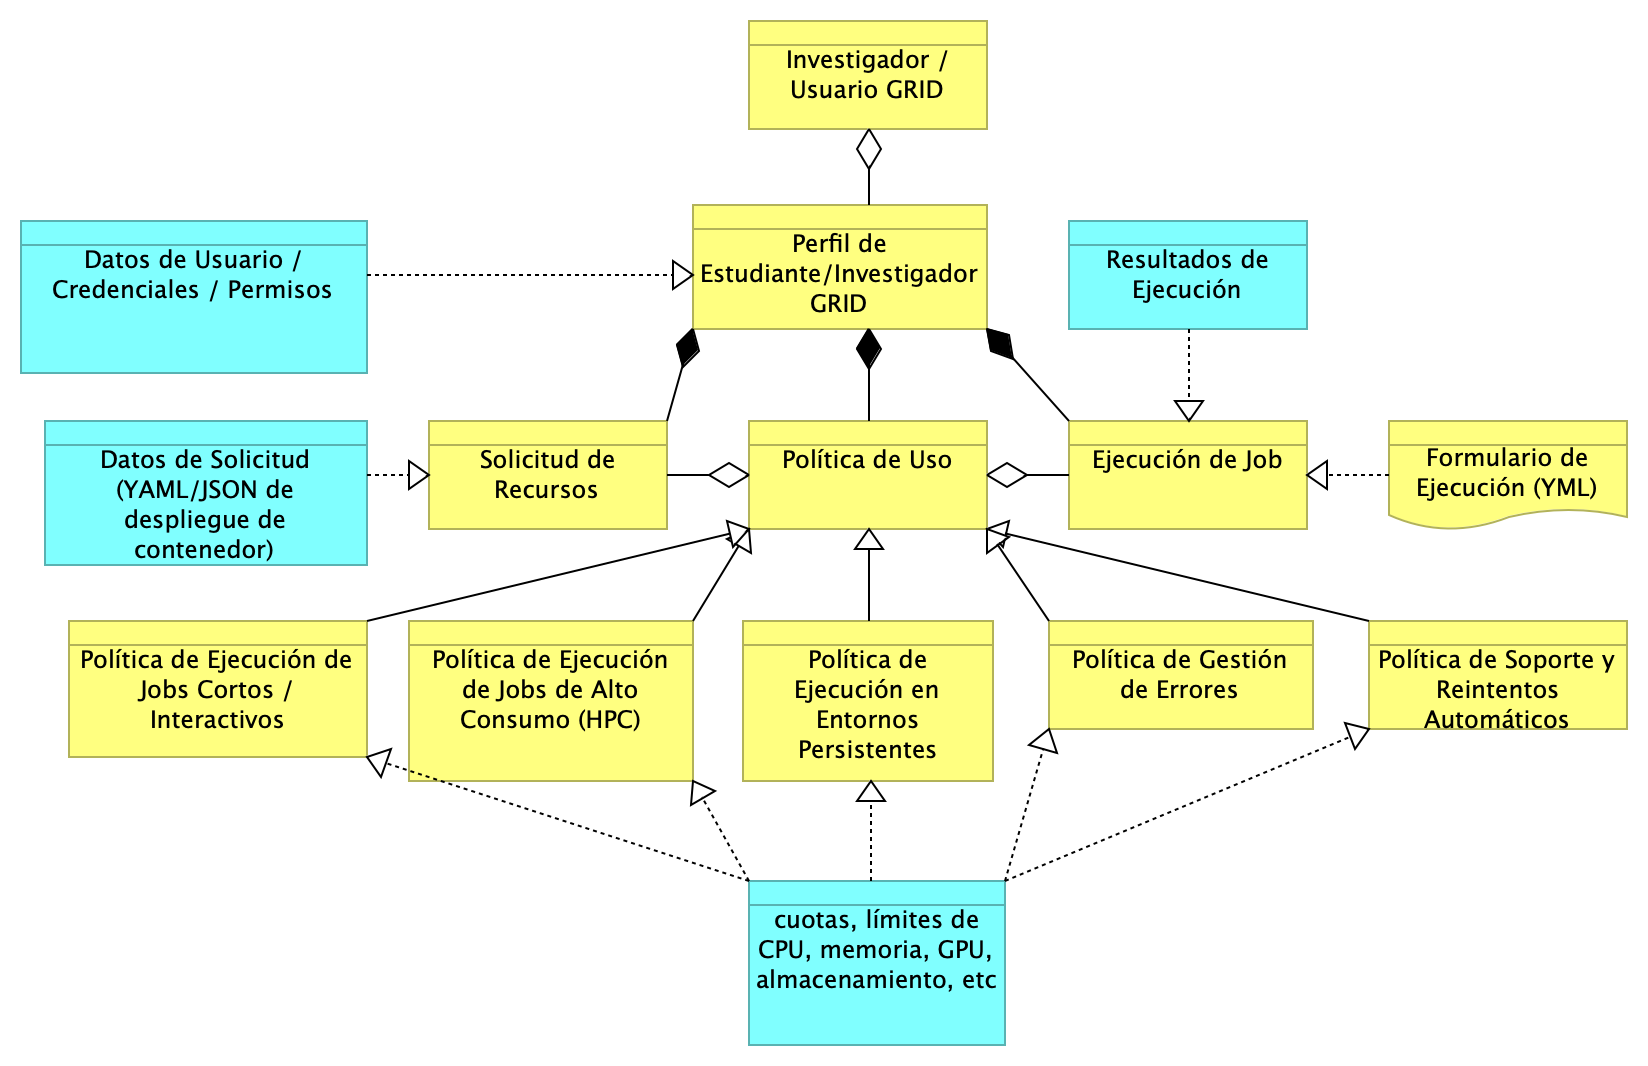
\includegraphics[width=\textwidth]{tablas-images/cp6/Information-Structure-View.png}
    \caption{Vista de Estructura de Información}
\end{figure}x


\subsection{Vista general}
\begin{figure}[H]
    \centering
    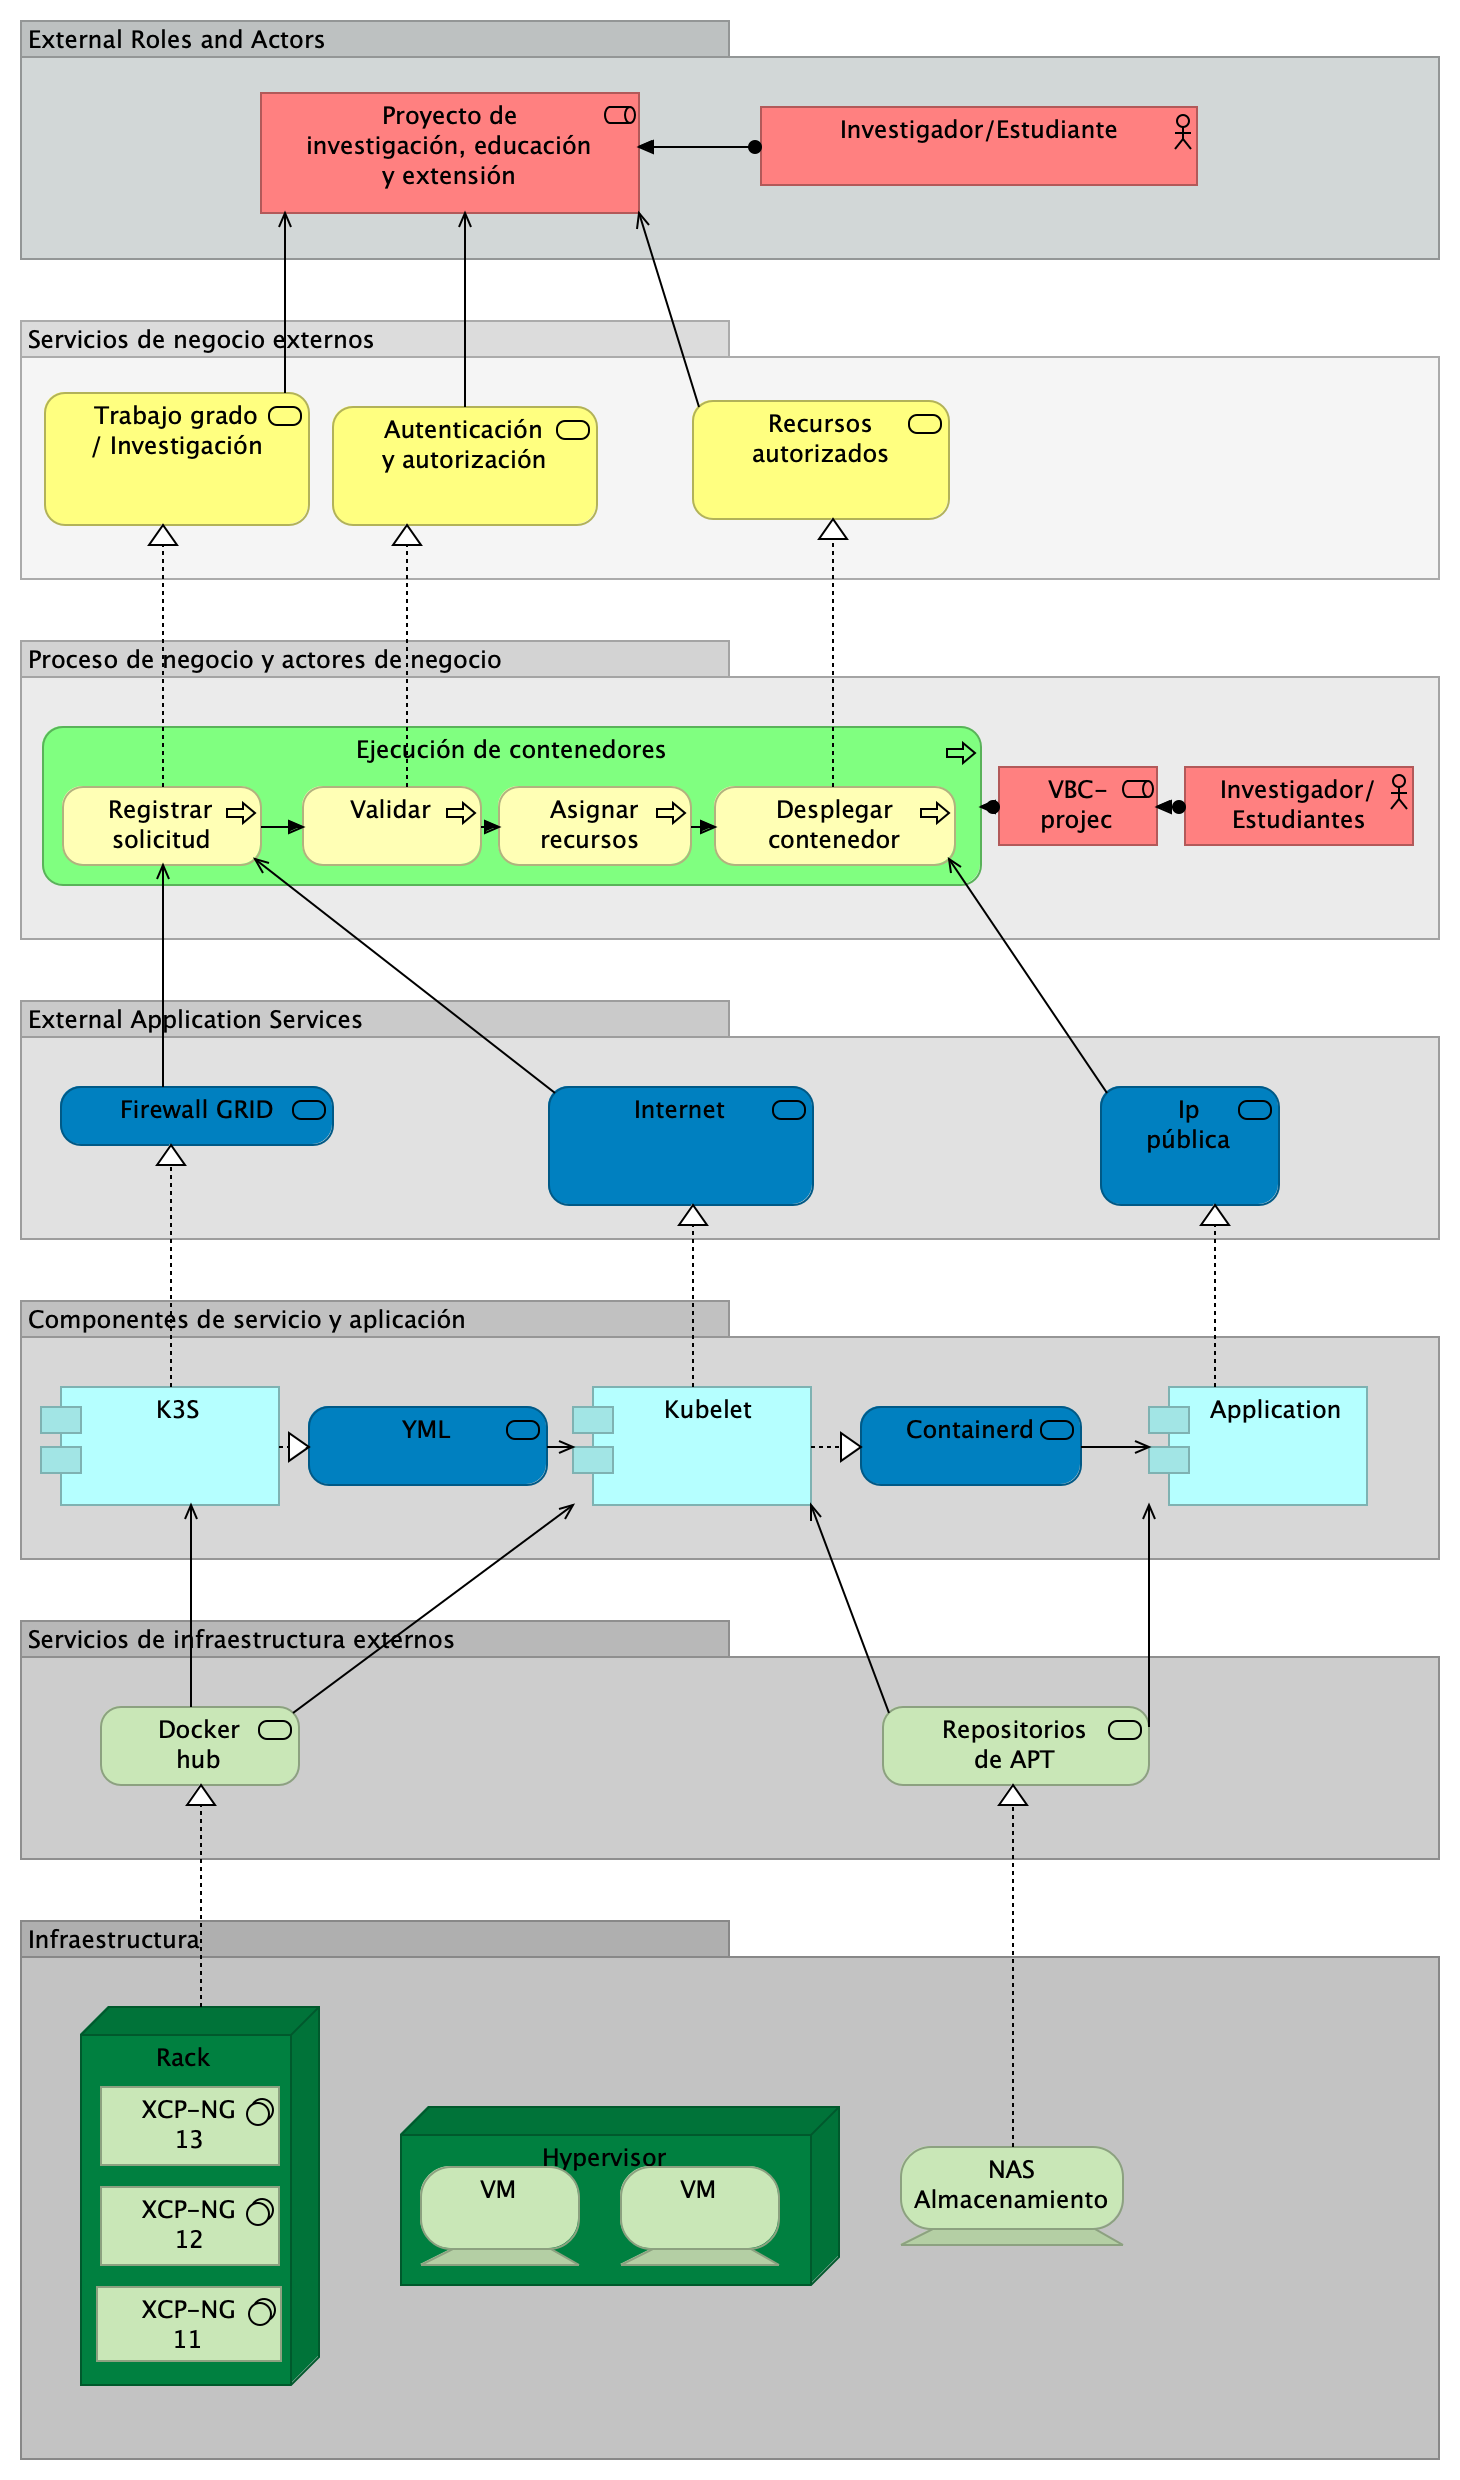
\includegraphics[scale=0.5]{tablas-images/cp6/Layered-View.png}
    \caption{Vista General en Capas}
\end{figure}

\section{Diseño por capas de la solución}

\section{Capa de infraestructura}

\begin{figure}[H]
    \centering
    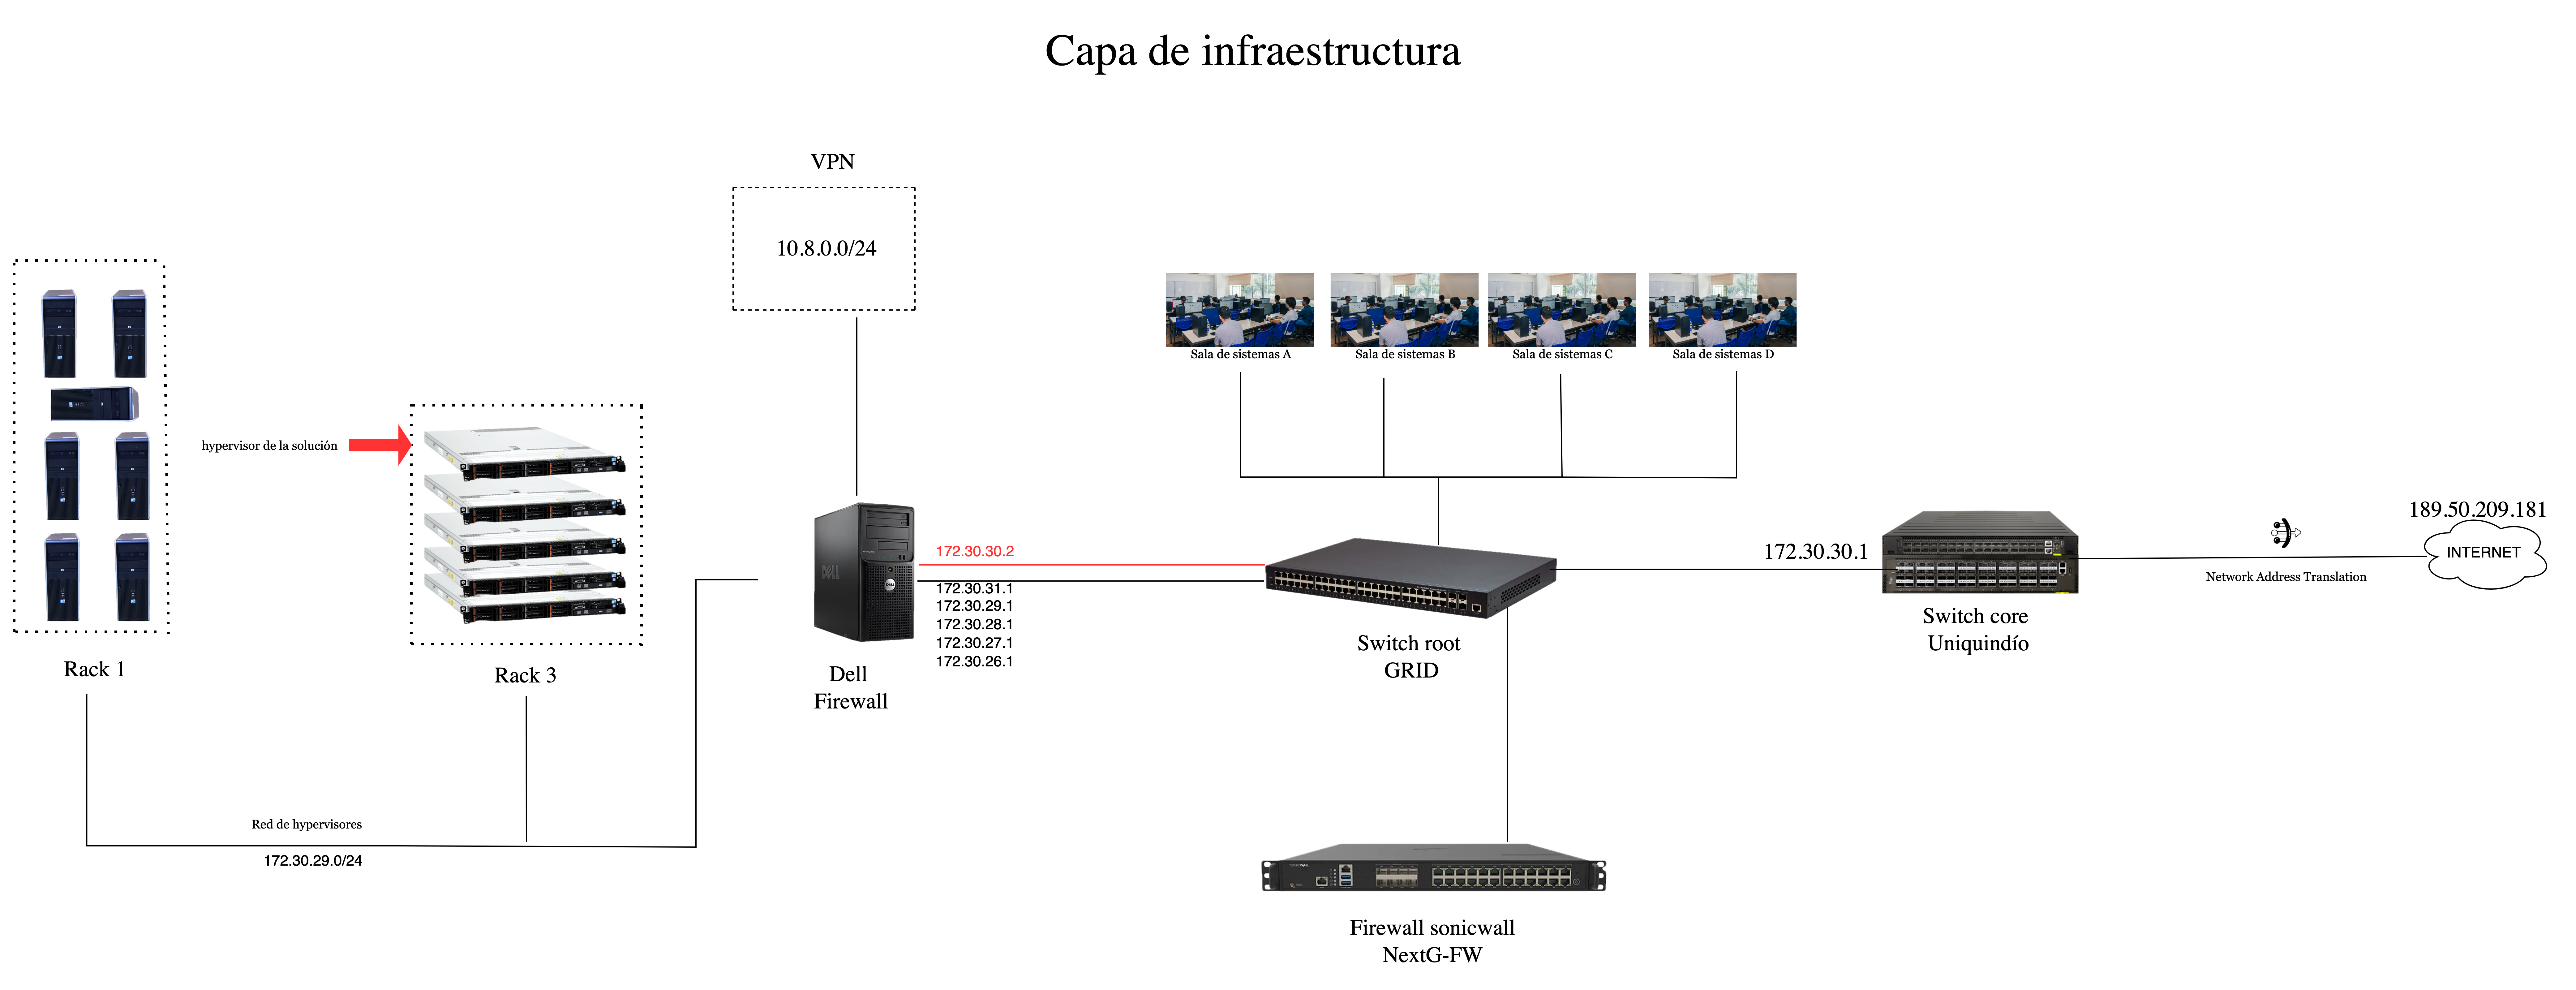
\includegraphics[width=\textwidth]{tablas-images/cp6/disenio-N1.png}
    \caption{Capa de Infraestructura}
\end{figure}

\section{Capa de virtualización}

\begin{figure}[H]
    \centering
    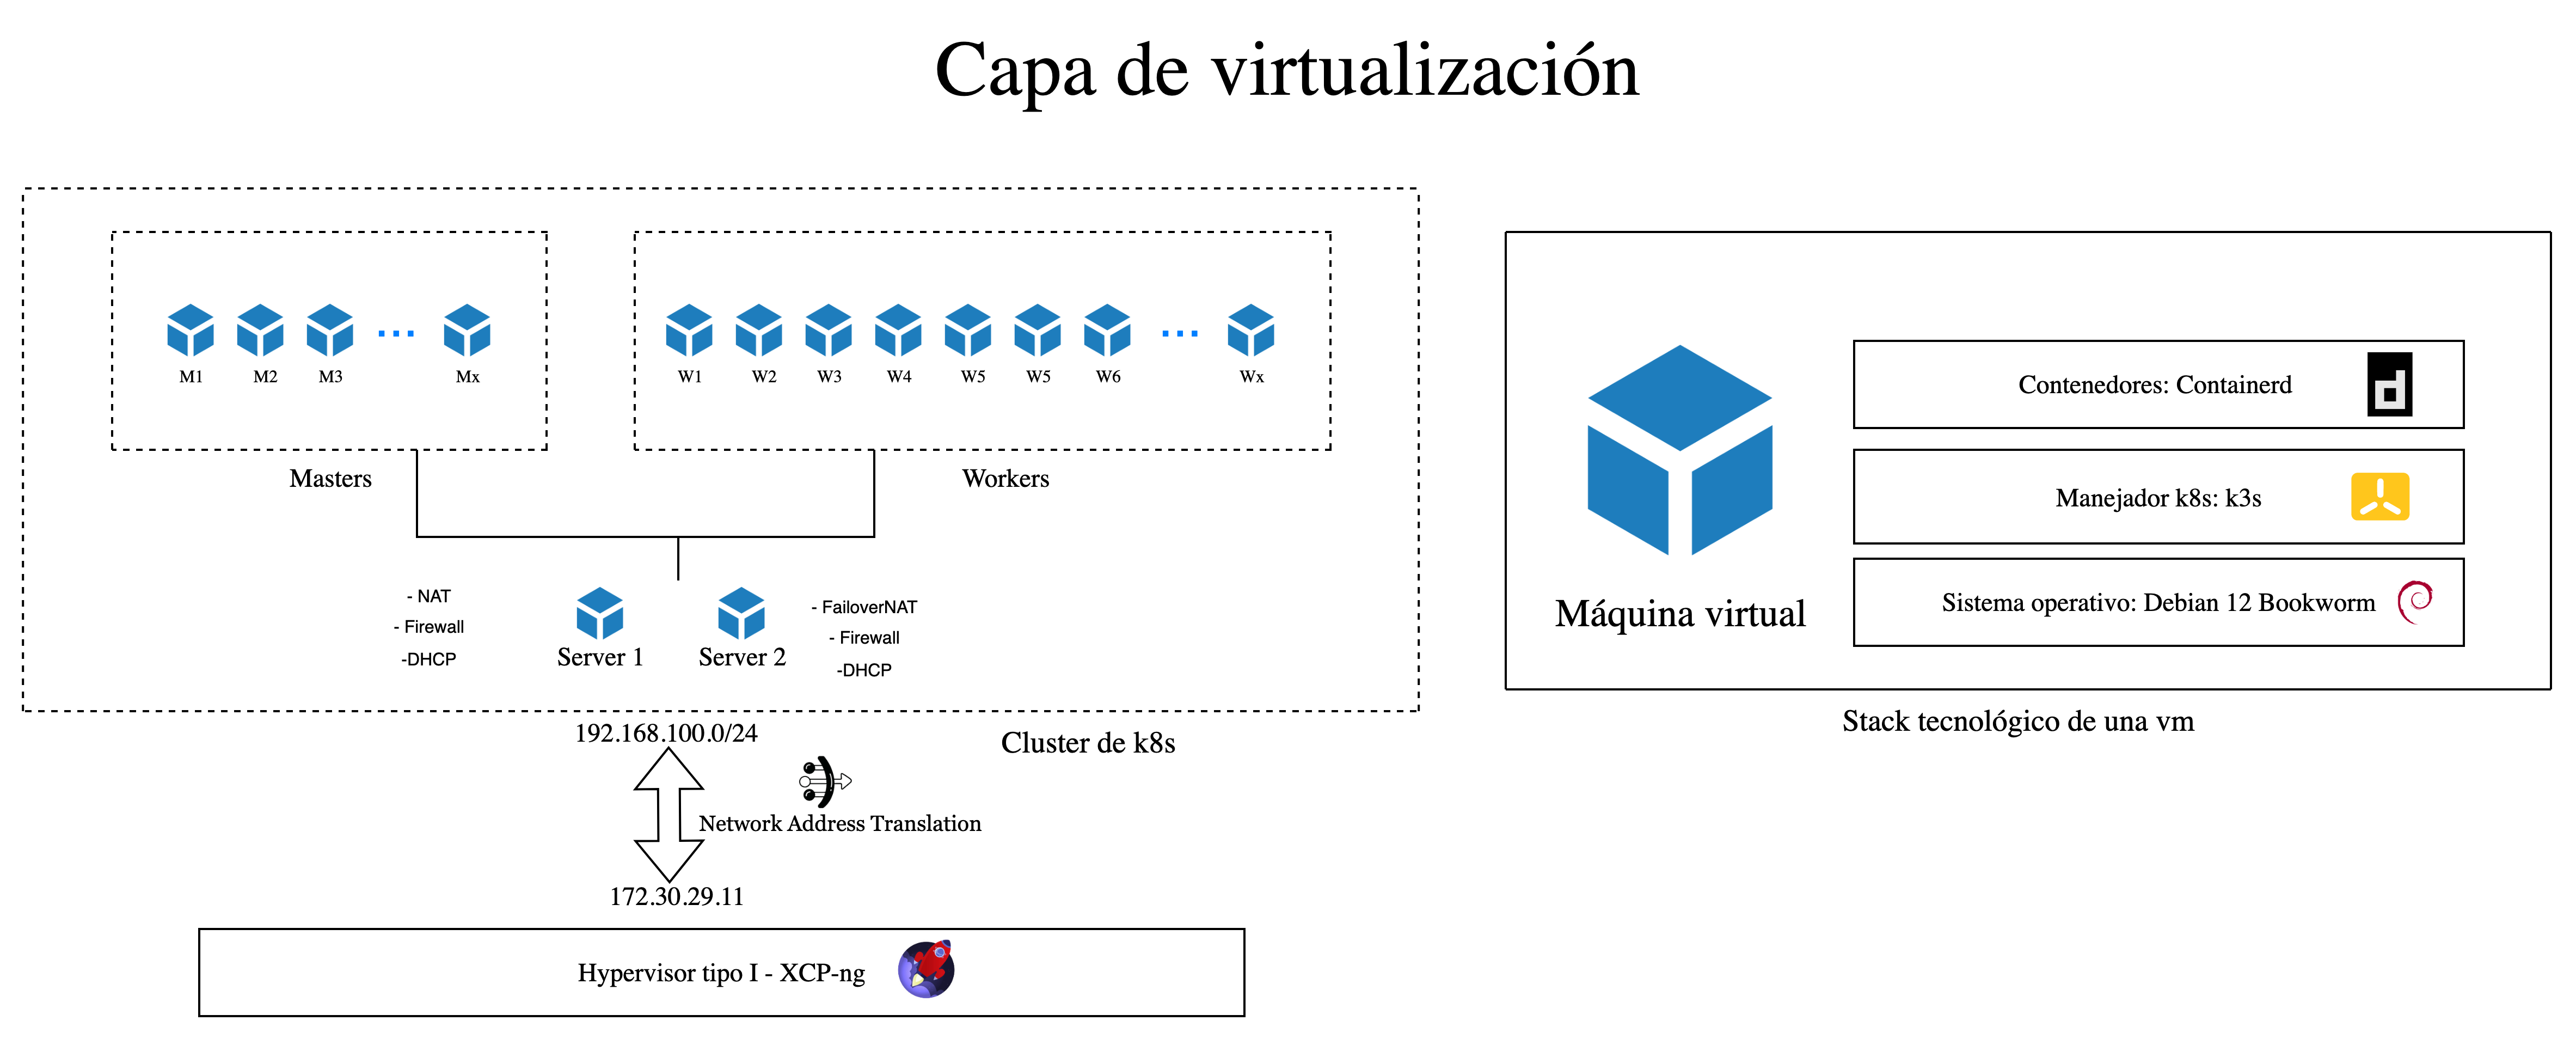
\includegraphics[width=\textwidth]{tablas-images/cp6/disenio-N2.png}
    \caption{Capa de Virtualización}
\end{figure}

\section{Capa de aplicación}


\ChapterImageStar[cap:cumplimiento-objetivos]{Cumplimiento de objetivos}{./images/fondo.png}\label{cap:cumplimiento-objetivos}

% Referencias - con imagen de fondo específica
\cleardoublepage\thispagestyle{empty}
\refstepcounter{chapter}
\phantomsection\addcontentsline{toc}{chapter}{Referencias}\label{cap:referencias}

% Imagen de fondo específica para referencias
\AddToShipoutPicture*{%
  \put(0,0){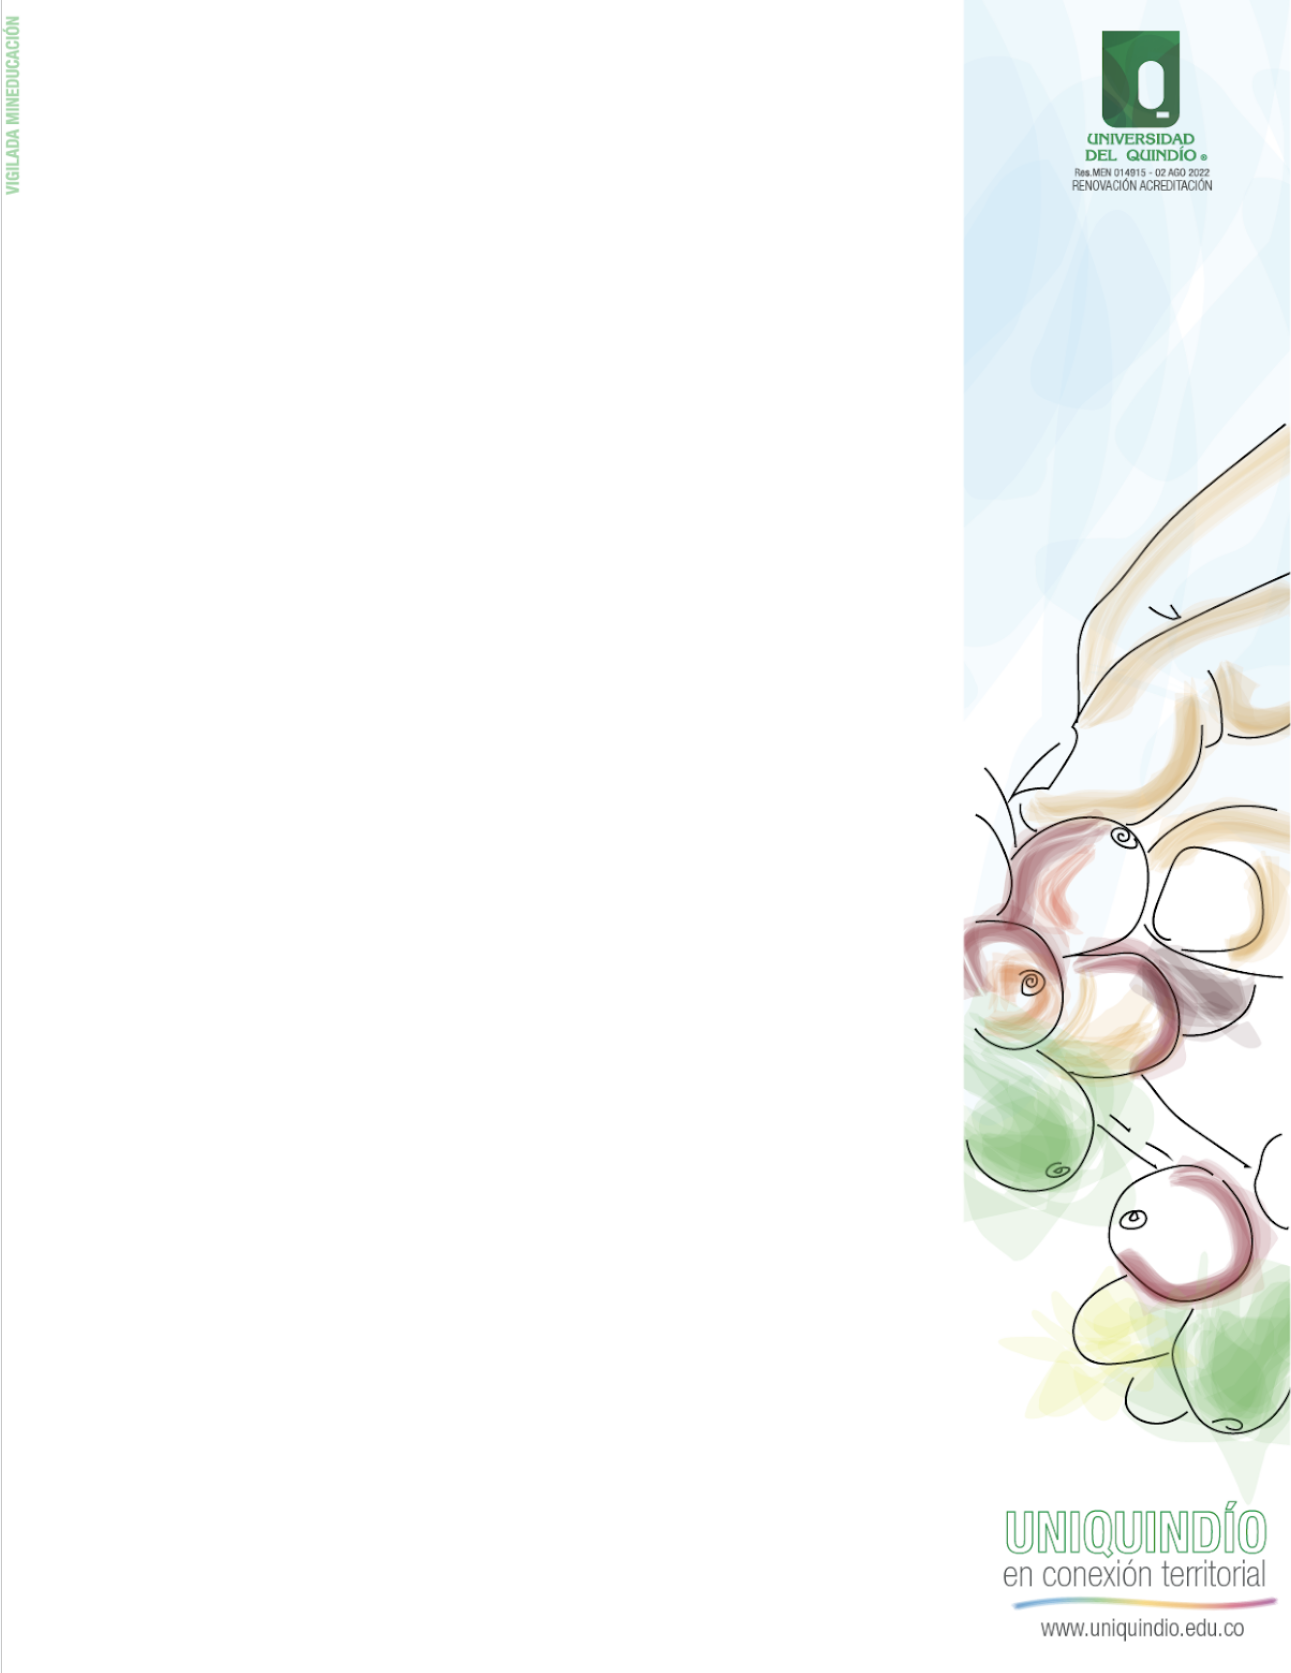
\includegraphics[width=\paperwidth,height=\paperheight]{./images/referencias.png}}%
}

% Título posicionado con coordenadas absolutas (en píxeles desde esquina superior izquierda)
\begin{tikzpicture}[remember picture,overlay]
  \node[anchor=north west] at ([xshift=150pt,yshift=-370pt]current page.north west)
    {\Large\bfseries\textcolor{black}{Referencias}};
\end{tikzpicture}
\vspace{2cm}

% Bibliografía sin título automático
\begingroup
  \renewcommand{\bibname}{}
  \pagestyle{fancy} % Fuerza el estilo fancy para todas las páginas de bibliografía
  \bibliographystyle{apalike}
  \bibliography{bibliografia}
\endgroup



\appendix

\chapter{Fichas técnicas y búsqueda en bases de datos}\label{apendice:fichas-y-busquedas}

\section{Ficha técnica del recurso tecnológico}
\begin{figure}[H]
    \centering
    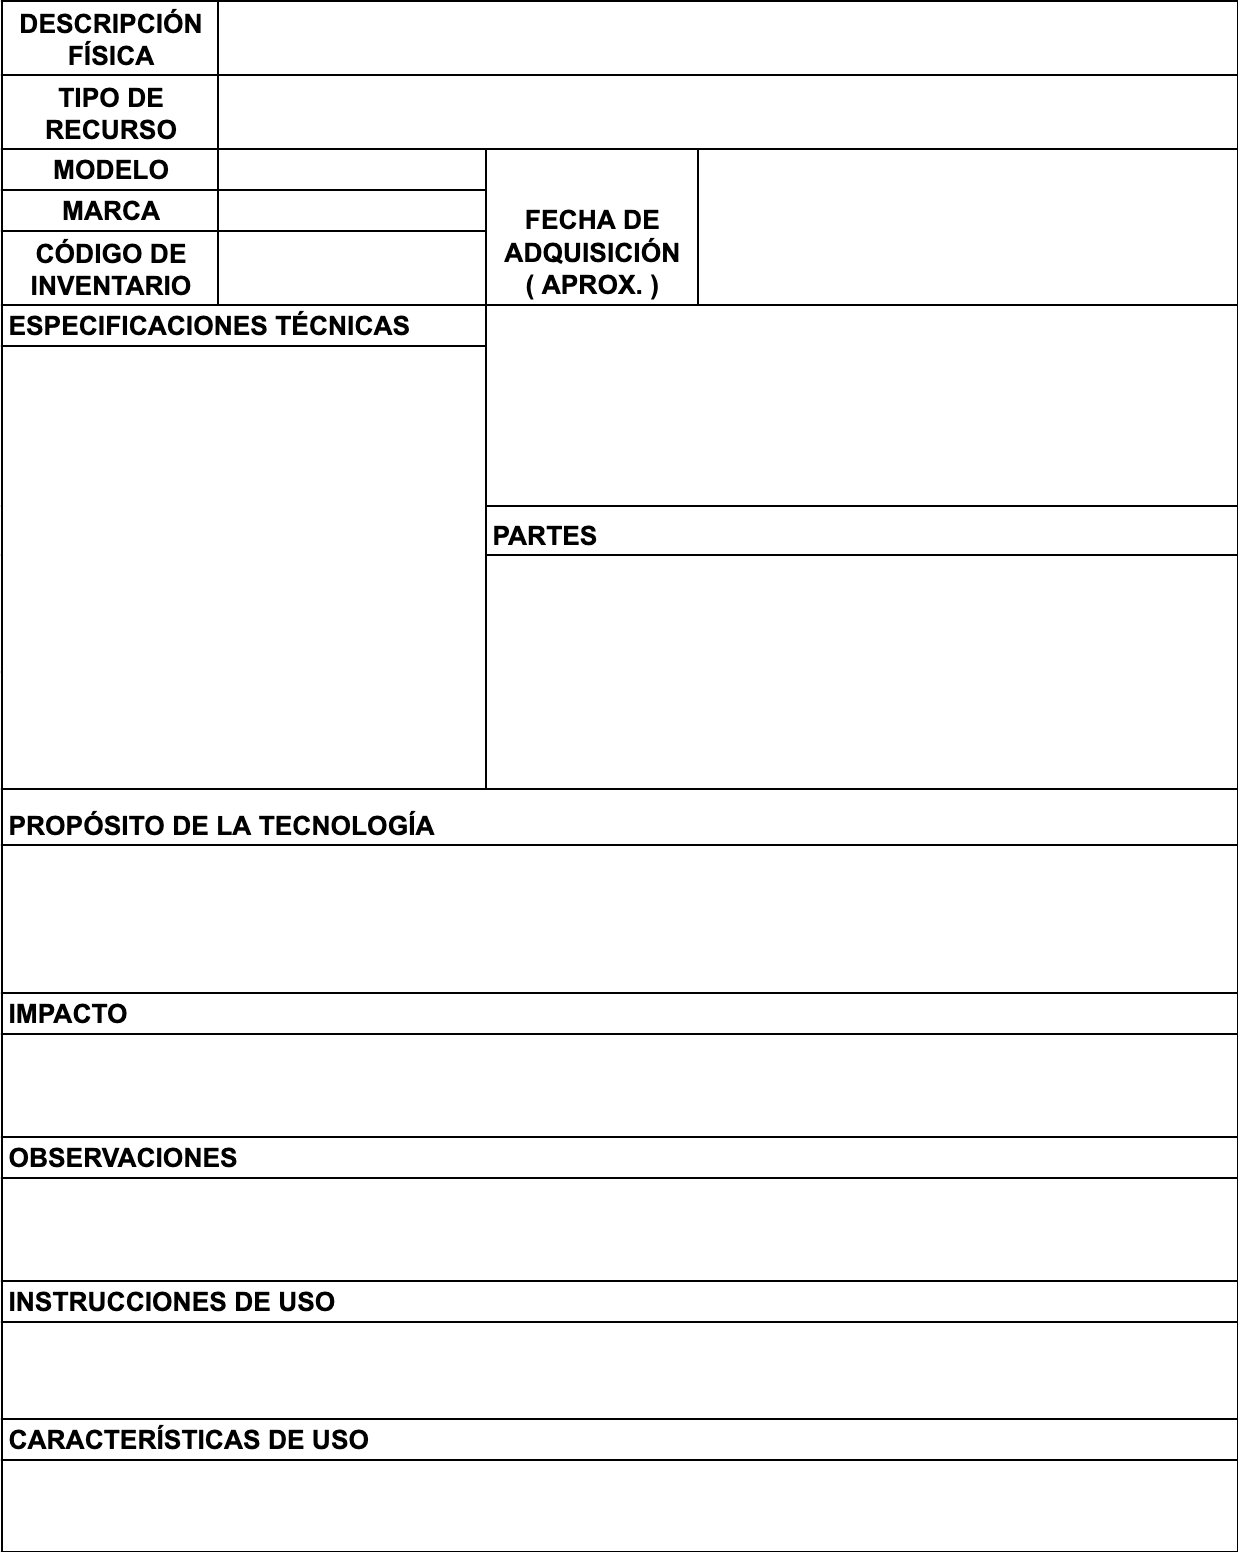
\includegraphics[width=\textwidth,height=0.85\textheight,keepaspectratio]{apendices/caracterizacionInfraestructura.png}
    \caption{Ficha técnica del recurso tecnológico}\label{fig:tabla-ficha-tecnica}
\end{figure}
\FloatBarrier\section*{Ficha técnica de servicios}

\begin{figure}[H]
    \centering
    \includegraphics[width=\textwidth,height=0.85\textheight,keepaspectratio]{apendices/caracterizacionServicios.png}
    \caption{Ficha técnica de servicios}\label{fig:tabla-ficha-servicios}
\end{figure}
\FloatBarrier\clearpage

\chapter{Búsquedas en bases de datos}

\section{Cadenas de búsqueda}\label{sec:cadenas-busqueda}


\begin{tcolorbox}[
  colback=gray!5, 
  colframe=black!60, 
  title=Cadena de búsqueda en ACM para educación, 
  fonttitle=\bfseries, 
  sharp corners=south
]
\scriptsize % o \footnotesize, \tiny según lo pequeño que lo quieras
\begin{verbatim}
(Title:("Container-based virtualization" OR "Application virtualization" OR "Docker" OR 
"Lightweight Virtualization") AND Title:("Education" OR "Education System" 
OR "Education Development" OR "Higher Education") ) 

OR

(Abstract:("Container-based virtualization" OR "Application virtualization" OR "Docker"
 OR "Lightweight Virtualization") AND Abstract:("Education" OR "Education System" 
 OR "Education Development" OR "Higher Education") )

OR

(Keyword:("Container-based virtualization" OR "Application virtualization" OR "Docker" OR 
"Lightweight Virtualization")
AND Keyword:("Education" OR "Education System" OR "Education Development" 
OR "Higher Education"))
\end{verbatim}
\end{tcolorbox}

\begin{tcolorbox}[
  colback=gray!5, 
  colframe=black!60, 
  title=Cadena de búsqueda en ACM para investigación, 
  fonttitle=\bfseries, 
  sharp corners=south
]
\scriptsize % puedes usar \tiny para hacerlo aún más pequeño
\begin{verbatim}
(Title:("Container-based virtualization" OR "Application virtualization" OR "Docker" OR 
"Lightweight Virtualization") AND Title:("Research" OR "Research Group" OR 
"Research Proposal"))

OR

(Abstract:("Container-based virtualization" OR "Application virtualization" OR "Docker" OR 
"Lightweight Virtualization") AND Abstract:("Research" OR "Research Group" OR 
"Research Proposal"))

OR

(Keyword:("Container-based virtualization" OR "Application virtualization" OR "Docker" OR 
"Lightweight Virtualization") AND Keyword:("Research" OR "Research Group" OR 
"Research Proposal"))
\end{verbatim}
\end{tcolorbox}

\begin{tcolorbox}[
  colback=gray!5, 
  colframe=black!60, 
  title=Cadena de búsqueda en ACM para extensión, 
  fonttitle=\bfseries, 
  sharp corners=south
]
\scriptsize % puedes usar \tiny para hacerlo aún más pequeño
\begin{verbatim}
(Title:("Container-based virtualization" OR "Application virtualization" OR "Docker" OR 
"Lightweight Virtualization") AND Title:("Industry" OR “IT Services” OR 
“Technology Infrastructure” OR “Cloud Computing”) ) 

OR

(Abstract:("Container-based virtualization" OR "Application virtualization" OR "Docker" 
OR "Lightweight Virtualization") AND Abstract:("Industry" OR “IT Services” OR 
“Technology Infrastructure” OR “Cloud Computing”) )

OR

(Keyword:("Container-based virtualization" OR "Application virtualization" OR "Docker" 
OR "Lightweight Virtualization")
AND Keyword:("Industry" OR “IT Services” OR “Technology Infrastructure” 
OR “Cloud Computing”))

\end{verbatim}
\end{tcolorbox}

\begin{tcolorbox}[
  colback=gray!5, 
  colframe=black!60, 
  title=Cadena de búsqueda en IEE para educación, 
  fonttitle=\bfseries, 
  sharp corners=south
]
\scriptsize % puedes usar \tiny para hacerlo aún más pequeño
\begin{verbatim}
(("Abstract":"Container-based virtualization" OR "Abstract":"Application virtualization" 
OR "Abstract":"Docker" OR "Abstract":"Lightweight Virtualization") AND ("Abstract":"Education" 
OR "Abstract":"Education System" OR "Abstract":"Education Development”  OR 
"Abstract":"Higher Education”)) 

OR (("Publication Title":"Container-based virtualization" OR "Publication 
Title":"Application virtualization" 
OR "Publication Title":"Docker" OR "Publication Title":"Lightweight Virtualization") 
AND ("Publication Title":"Education" 
OR "Publication Title":"Education System" OR "Publication Title":"Education Development”  
OR "Publication Title":"Higher Education” ))

OR (("Author Keywords":"Container-based virtualization" OR 
"Author Keywords":"Application virtualization" OR 
"Author Keywords":"Docker" OR "Author Keywords":"Lightweight Virtualization") AND 
("Author Keywords":"Education" 
OR "Author Keywords":"Education System" OR "Author Keywords":"Education Development”  
OR "Author Keywords":"Higher Education”))
\end{verbatim}
\end{tcolorbox}


\begin{tcolorbox}[
  colback=gray!5, 
  colframe=black!60, 
  title=Cadena de búsqueda en IEE para investigación, 
  fonttitle=\bfseries, 
  sharp corners=south
]
\scriptsize % puedes usar \tiny para hacerlo aún más pequeño
\begin{verbatim}
(("Abstract":"Container-based virtualization" OR "Abstract":"Application virtualization" 
OR "Abstract":"Docker" OR "Abstract":"Lightweight Virtualization") AND 
("Abstract":"Research Group" OR "Abstract":"Research Proposal")) 

OR (("Publication Title":"Container-based virtualization" OR 
"Publication Title":"Application virtualization" OR "Publication Title":"Docker" OR 
"Publication Title":"Lightweight Virtualization") AND 
("Publication Title":"Research Group" OR "Publication Title":"Research Proposal" ))

OR (("Author Keywords":"Container-based virtualization" OR 
"Author Keywords":"Application virtualization" OR "Author Keywords":"Docker" OR 
"Author Keywords":"Lightweight Virtualization") AND 
("Author Keywords":"Research Group" OR "Author Keywords":"Research Proposal"))
\end{verbatim}
\end{tcolorbox}

\begin{tcolorbox}[
  colback=gray!5, 
  colframe=black!60, 
  title=Cadena de búsqueda en IEE para extensión, 
  fonttitle=\bfseries, 
  sharp corners=south
]
\scriptsize % puedes usar \tiny para hacerlo aún más pequeño
\begin{verbatim}
(("Abstract":"Container-based virtualization" OR "Abstract":"Application virtualization" 
OR "Abstract":"Docker" OR "Abstract":"Lightweight Virtualization") AND 
("Abstract":"Industry" OR "Abstract":"IT Services" OR 
"Abstract":"Technology Infrastructure" OR "Abstract":"Cloud Computing")) 

OR (("Publication Title":"Container-based virtualization" OR 
"Publication Title":"Application virtualization" 
OR "Publication Title":"Docker" OR "Publication Title":"Lightweight Virtualization") AND 
("Publication Title":"Industry" OR "Publication Title":"IT Services" OR 
"Publication Title":"Technology Infrastructure" OR "Publication Title":"Cloud Computing"))

OR (("Author Keywords":"Container-based virtualization" OR 
"Author Keywords":"Application virtualization" OR "Author Keywords":"Docker" OR 
"Author Keywords":"Lightweight Virtualization") AND ("Author Keywords":"Industry" OR 
"Author Keywords":"IT Services" OR "Author Keywords":"Technology Infrastructure" OR 
"Author Keywords":"Cloud Computing"))
\end{verbatim}
\end{tcolorbox}

\begin{tcolorbox}[
  colback=gray!5, 
  colframe=black!60, 
  title=Cadena de búsqueda en Springer para educación, 
  fonttitle=\bfseries, 
  sharp corners=south
]
\scriptsize % puedes usar \tiny para hacerlo aún más pequeño
\begin{verbatim}
(title:("Container-based virtualization" OR "Application virtualization" OR 
"Docker" OR "Lightweight Virtualization") AND title:("Education" OR 
"Education System" OR "Education Development" OR "Higher Education"))

OR

(abstract:("Container-based virtualization" OR "Application virtualization" OR 
"Docker" OR "Lightweight Virtualization") AND abstract:("Education" OR 
"Education System" OR "Education Development" OR "Higher Education"))

OR 

(keyword:("Container-based virtualization" OR "Application virtualization" OR 
"Docker" OR "Lightweight Virtualization") AND keyword:("Education" OR 
"Education System" OR "Education Development" OR "Higher Education"))

\end{verbatim}
\end{tcolorbox}

\begin{tcolorbox}[
  colback=gray!5, 
  colframe=black!60, 
  title=Cadena de búsqueda en Springer para investigación, 
  fonttitle=\bfseries, 
  sharp corners=south
]
\scriptsize % puedes usar \tiny para hacerlo aún más pequeño
\begin{verbatim}
(title:("Container-based virtualization" OR "Application virtualization" OR 
"Docker" OR "Lightweight Virtualization") AND title:("research" OR 
"Research Group" OR "Research Proposal"))

OR

(abstract:("Container-based virtualization" OR "Application virtualization" 
OR "Docker" OR "Lightweight Virtualization") AND abstract:("research" 
OR "Research Group" OR "Research Proposal"))

OR 

(keyword:("Container-based virtualization" OR "Application virtualization"
 OR "Docker" OR "Lightweight Virtualization") AND keyword:("research" OR 
 "Research Group" OR "Research Proposal"))

\end{verbatim}
\end{tcolorbox}

\begin{tcolorbox}[
  colback=gray!5, 
  colframe=black!60, 
  title=Cadena de búsqueda en Springer para extensión, 
  fonttitle=\bfseries, 
  sharp corners=south
]
\scriptsize % puedes usar \tiny para hacerlo aún más pequeño
\begin{verbatim}
(title:("Container-based virtualization" OR "Application virtualization"
 OR "Docker" OR "Lightweight Virtualization") AND title:("Industry" OR 
 “IT Services” OR “Technology Infrastructure” OR “Cloud Computing”))

OR

(abstract:("Container-based virtualization" OR "Application virtualization" 
OR "Docker" OR "Lightweight Virtualization") AND abstract:("Industry" OR 
“IT Services” OR “Technology Infrastructure” OR “Cloud Computing”))

OR 

(keyword:("Container-based virtualization" OR "Application virtualization"
 OR "Docker" OR "Lightweight Virtualization") AND keyword:("Industry" 
 OR “IT Services” OR “Technology Infrastructure” OR “Cloud Computing”))

\end{verbatim}
\end{tcolorbox}

\begin{tcolorbox}[
  colback=gray!5, 
  colframe=black!60, 
  title=Cadena de búsqueda en Science Direct para educación, 
  fonttitle=\bfseries, 
  sharp corners=south
]
\scriptsize % puedes usar \tiny para hacerlo aún más pequeño
\begin{verbatim}
("Container-based virtualization" OR "Application virtualization" 
OR "Docker" OR "Lightweight Virtualization")  AND ("Education" OR 
"Education System" OR "Education Development" OR "Higher Education")
\end{verbatim}
\end{tcolorbox}


\begin{tcolorbox}[
  colback=gray!5, 
  colframe=black!60, 
  title=Cadena de búsqueda en Science Direct para investigación, 
  fonttitle=\bfseries, 
  sharp corners=south
]
\scriptsize % puedes usar \tiny para hacerlo aún más pequeño
\begin{verbatim}
("Container-based virtualization" OR "Application virtualization" OR 
"Docker" OR "Lightweight Virtualization")  AND ("Research" OR 
"Research Group" OR "Research Proposal")
\end{verbatim}
\end{tcolorbox}

\begin{tcolorbox}[
  colback=gray!5, 
  colframe=black!60, 
  title=Cadena de búsqueda en Science Direct para extensión, 
  fonttitle=\bfseries, 
  sharp corners=south
]
\scriptsize % puedes usar \tiny para hacerlo aún más pequeño
\begin{verbatim}
("Container-based virtualization" OR "Application virtualization" OR "Docker" OR 
"Lightweight Virtualization")  AND 
(“Industry” OR "IT Services" OR "Technology Infrastructure" OR "Cloud Computing")
\end{verbatim}
\end{tcolorbox}

\begin{tcolorbox}[
  colback=gray!5, 
  colframe=black!60, 
  title=Cadena de búsqueda en Taylor \& Francis para educación, 
  fonttitle=\bfseries, 
  sharp corners=south
]
\scriptsize % puedes usar \tiny para hacerlo aún más pequeño
\begin{verbatim}
("Application virtualization" OR "Docker" OR "Lightweight Virtualization" OR "Docker Container")   
AND   
("Education System" OR "Education Sector" OR "Education Development" OR "Higher Education")
\end{verbatim}
\end{tcolorbox}

\begin{tcolorbox}[
  colback=gray!5, 
  colframe=black!60, 
  title=Cadena de búsqueda en Taylor \& Francis para investigación, 
  fonttitle=\bfseries, 
  sharp corners=south
]
\scriptsize % puedes usar \tiny para hacerlo aún más pequeño
\begin{verbatim}
("Application virtualization" OR "Docker" OR "Lightweight Virtualization" OR "Docker Container")
AND   
("Specific Research Areas" OR "Research Group" OR "Research Proposal" OR "Research and Development")
\end{verbatim}
\end{tcolorbox}

\begin{tcolorbox}[
  colback=gray!5, 
  colframe=black!60, 
  title=Cadena de búsqueda en Taylor \& Francis para extensión, 
  fonttitle=\bfseries, 
  sharp corners=south
]
\scriptsize % puedes usar \tiny para hacerlo aún más pequeño
\begin{verbatim}
("Application virtualization" OR "Docker" OR "Lightweight Virtualization" OR "Docker Container")  
AND 
(“Industry” OR "IT Services" OR "Technology Infrastructure" OR "Cloud Computing")
\end{verbatim}
\end{tcolorbox}


\section{Búsqueda de artículos sin criterios de inclusión/exclusión}

\begin{figure}[H]
    \centering
    \includegraphics[width=\textwidth,keepaspectratio]{apendices/BD/sin-criterios/ACM-ed.png}
    \caption{Búsqueda de artículos de educación en ACM sin criterios de inclusión/exclusión \\
    Fecha de acceso: 12/03/25 9:13 pm
    }\label{fig:busqueda1}
\end{figure}
\FloatBarrier\begin{figure}[H]
    \centering
    \includegraphics[width=\textwidth,keepaspectratio]{apendices/BD/sin-criterios/ACM-inv.png}
    \caption{Búsqueda de artículos de investigación en ACM sin criterios de inclusión/exclusión \\
    Fecha de acceso: 12/03/25 8:23 pm
    }\label{fig:busqueda2}
\end{figure}
\FloatBarrier\begin{figure}[H]
    \centering
    \includegraphics[width=\textwidth,keepaspectratio]{apendices/BD/sin-criterios/ACM-ind.png}
    \caption{Búsqueda de artículos de extensión en ACM sin criterios de inclusión/exclusión \\
    Fecha de acceso: 12/03/25 9:20 pm
    }\label{fig:busqueda3}
\end{figure}
\FloatBarrier\begin{figure}[H]
    \centering
    \includegraphics[width=\textwidth,keepaspectratio]{apendices/BD/sin-criterios/IEEE-ed.png}
    \caption{Búsqueda de artículos de educación en IEEE sin criterios de inclusión/exclusión
    Fecha de acceso: 7/03/25 8:50 pm
    }\label{fig:busqueda4}
\end{figure}
\FloatBarrier\begin{figure}[H]
    \centering
    \includegraphics[width=\textwidth,keepaspectratio]{apendices/BD/sin-criterios/IEEE-inv.png}
    \caption{Búsqueda de artículos de investigación en IEEE sin criterios de inclusión/exclusión
    Fecha de acceso: 7/03/25 8:46 pm
    }\label{fig:busqueda5}
\end{figure}
\FloatBarrier\begin{figure}[H]
    \centering
    \includegraphics[width=\textwidth,keepaspectratio]{apendices/BD/sin-criterios/IEEE-ind.png}
    \caption{Búsqueda de artículos de extensión en IEEE sin criterios de inclusión/exclusión
    Fecha de acceso: 12/03/25 8:54 pm
    }\label{fig:busqueda6}
\end{figure}
\FloatBarrier\begin{figure}[H]
    \centering
    \includegraphics[width=\textwidth,keepaspectratio]{apendices/BD/sin-criterios/Springer-ed.png}
    \caption{Búsqueda de artículos de educación en Springer sin criterios de inclusión/exclusión
    Fecha de acceso: 12/03/25 9:58 pm
    }\label{fig:busqueda7}
\end{figure}
\FloatBarrier\begin{figure}[H]
    \centering
    \includegraphics[width=\textwidth,keepaspectratio]{apendices/BD/sin-criterios/Springer-inv.png}
    \caption{Búsqueda de artículos de investigación en Springer sin criterios de inclusión/exclusión
    Fecha de acceso: 13/03/25 12:40 pm
    }\label{fig:busqueda8}
\end{figure}
\FloatBarrier\begin{figure}[H]
    \centering
    \includegraphics[width=\textwidth,keepaspectratio]{apendices/BD/sin-criterios/Springer-ind.png}
    \caption{Búsqueda de artículos de extensión en Springer sin criterios de inclusión/exclusión
    Fecha de acceso: 13/03/25 12:48 pm}\label{fig:busqueda9}
\end{figure}
\FloatBarrier\begin{figure}[H]
    \centering
    \includegraphics[width=\textwidth,keepaspectratio]{apendices/BD/sin-criterios/SD-ed.png}
    \caption{Búsqueda de artículos de educación en Science Direct sin criterios de inclusión/exclusión
    Fecha de acceso: 13/03/25 1:03 pm}\label{fig:busqueda10}
\end{figure}
\FloatBarrier\begin{figure}[H]
    \centering
    \includegraphics[width=\textwidth,keepaspectratio]{apendices/BD/sin-criterios/SD-inv.png}
    \caption{Búsqueda de artículos de investigación en Science Direct sin criterios de inclusión/exclusión
    Fecha de acceso: 13/03/25 1:43 pm}\label{fig:busqueda11}
\end{figure}
\FloatBarrier\begin{figure}[H]
    \centering
    \includegraphics[width=\textwidth,keepaspectratio]{apendices/BD/sin-criterios/SD-ind.png}
    \caption{Búsqueda de artículos de extensión en Science Direct sin criterios de inclusión/exclusión
    Fecha de acceso: 13/03/25 1:48 pm}\label{fig:busqueda12}
\end{figure}
\FloatBarrier\begin{figure}[H]
    \centering
    \includegraphics[width=\textwidth,keepaspectratio]{apendices/BD/sin-criterios/TF-ed.png}
    \caption{Búsqueda de artículos de educación en Taylor \& Francis sin criterios de inclusión/exclusión
    Fecha de acceso: 16/03/25 9:21 pm}\label{fig:busqueda13}
\end{figure}
\FloatBarrier\begin{figure}[H]
    \centering
    \includegraphics[width=\textwidth,keepaspectratio]{apendices/BD/sin-criterios/TF-inv.png}
    \caption{Búsqueda de artículos de investigación en Taylor \& Francis sin criterios de inclusión/exclusión
    Fecha de acceso: 16/03/25 9:31 pm
    }\label{fig:busqueda14}
\end{figure}
\FloatBarrier\begin{figure}[H]
    \centering
    \includegraphics[width=\textwidth,keepaspectratio]{apendices/BD/sin-criterios/TF-ind.png}
    \caption{Búsqueda de artículos de extensión en Taylor \& Francis sin criterios de inclusión/exclusión
    Fecha de acceso: 16/03/25 9:34 pm
    }\label{fig:busqueda15}
\end{figure}
\FloatBarrier\section{Búsqueda de artículos usando criterios de inclusión/exclusión}
\begin{figure}[H]
    \centering
    \includegraphics[width=\textwidth,keepaspectratio]{apendices/BD/criterios/ACM-ed.png}
    \caption{Búsqueda de artículos de educación en ACM con criterios de inclusión/exclusión
    Fecha de acceso: 20/03/25 1:15 pm
    }\label{fig:busqueda16}
\end{figure}
\FloatBarrier\begin{figure}[H]
    \centering
    \includegraphics[width=\textwidth,keepaspectratio]{apendices/BD/criterios/ACM-inv.png}
    \caption{Búsqueda de artículos de investigación en ACM con criterios de inclusión/exclusión
    Fecha de acceso: 20/03/25 1:19 pm
    }\label{fig:busqueda17}
\end{figure}
\FloatBarrier\begin{figure}[H]
    \centering
    \includegraphics[width=\textwidth,keepaspectratio]{apendices/BD/criterios/ACM-ind.png}
    \caption{Búsqueda de artículos de extensión en ACM con criterios de inclusión/exclusión
    Fecha de acceso: 20/03/25 1:20 pm
    }\label{fig:busqueda18}
\end{figure}
\FloatBarrier\begin{figure}[H]
    \centering
    \includegraphics[width=\textwidth,keepaspectratio]{apendices/BD/criterios/IEEE-ed.png}
    \caption{Búsqueda de artículos de educación en IEEE con criterios de inclusión/exclusión
    Fecha de acceso: 20/03/25 1:27 pm
    }\label{fig:busqueda19}
\end{figure}
\FloatBarrier\begin{figure}[H]
    \centering
    \includegraphics[width=\textwidth,keepaspectratio]{apendices/BD/criterios/IEEE-ind.png}
    \caption{Búsqueda de artículos de extensión en IEEE con criterios de inclusión/exclusión
    Fecha de acceso: 20/03/25 1:37 pm
    }\label{fig:busqueda21}
\end{figure}
\FloatBarrier\begin{figure}[H]
    \centering
    \includegraphics[width=\textwidth,keepaspectratio]{apendices/BD/criterios/Springer-ed.png}
    \caption{Búsqueda de artículos de educación en Springer con criterios de inclusión/exclusión
    Fecha de acceso: 20/03/25 2:29 pm
    }\label{fig:busqueda22}
\end{figure}
\FloatBarrier\begin{figure}[H]
    \centering
    \includegraphics[width=\textwidth,keepaspectratio]{apendices/BD/criterios/Springer-inv.png}
    \caption{Búsqueda de artículos de investigación en Springer con criterios de inclusión/exclusión
    Fecha de acceso: 16/03/25 11:05 am
    }\label{fig:busqueda23}
\end{figure}
\FloatBarrier\begin{figure}[H]
    \centering
    \includegraphics[width=\textwidth,keepaspectratio]{apendices/BD/criterios/Springer-ind.png}
    \caption{Búsqueda de artículos de extensión en Springer con criterios de inclusión/exclusión
    Fecha de acceso: 16/03/25 11:07 am
    }\label{fig:busqueda24}
\end{figure}
\FloatBarrier\begin{figure}[H]
    \centering
    \includegraphics[width=\textwidth,keepaspectratio]{apendices/BD/criterios/SD-ed.png}
    \caption{Búsqueda de artículos de educación en Science Direct con criterios de inclusión/exclusión
    Fecha de acceso: 20/03/25 2:59 am
    }\label{fig:busqueda25}
\end{figure}
\FloatBarrier\begin{figure}[H]
    \centering
    \includegraphics[width=\textwidth,keepaspectratio]{apendices/BD/criterios/SD-inv.png}
    \caption{Búsqueda de artículos de investigación en Science Direct con criterios de inclusión/exclusión
    Fecha de acceso: 20/03/25 3:01 am
    }\label{fig:busqueda26}
\end{figure}
\FloatBarrier\begin{figure}[H]
    \centering
    \includegraphics[width=\textwidth,keepaspectratio]{apendices/BD/criterios/SD-ind.png}
    \caption{Búsqueda de artículos de extensión en Science Direct con criterios de inclusión/exclusión
    Fecha de acceso: 20/03/25 3:07 am
    }\label{fig:busqueda27}
\end{figure}
\FloatBarrier\begin{figure}[H]
    \centering
    \includegraphics[width=\textwidth,keepaspectratio]{apendices/BD/criterios/TF-ed.png}
    \caption{Búsqueda de artículos de educación en Taylor \& Francis con criterios de inclusión/exclusión
    Fecha de acceso: 20/03/25 4:46 am
    }\label{fig:busqueda28}
\end{figure}
\FloatBarrier\begin{figure}[H]
    \centering
    \includegraphics[width=\textwidth,keepaspectratio]{apendices/BD/criterios/TF-inv.png}
    \caption{Búsqueda de artículos de investigación en Taylor \& Francis con criterios de inclusión/exclusión
    Fecha de acceso: 20/03/25 4:49 am
    }\label{fig:busqueda29}
\end{figure}
\FloatBarrier\begin{figure}[H]
    \centering
    \includegraphics[width=\textwidth,keepaspectratio]{apendices/BD/criterios/TF-ind.png}
    \caption{Búsqueda de artículos de extensión en Taylor \& Francis con criterios de inclusión/exclusión
    Fecha de acceso: 20/03/25 4:50 am
    }\label{fig:busqueda30}
\end{figure}
\FloatBarrier\chapter{Plantilla del análisis DAR}
\section{Plantilla análisis DAR}

\begin{figure}[H]
    \centering
    \includegraphics[width=\textwidth,height=0.85\textheight,keepaspectratio]{apendices/plantilla-DAR.png}
    \caption{Plantilla del análisis DAR}\label{fig:tabla-plantilla-dar}
\end{figure}
\FloatBarrier\chapter{Eventos de difusión}
\section{Seminario GRID 2024-II}


\section{Seminario GRID 2025-I}

\section{ACOFI 2025}

En esta sección se presenta la ponencia presentada en el congreso ACOFI 2025 como resultado de la investigación desarrollada en este trabajo.

\subsection{Páginas de la ponencia ACOFI}

% Página 1
\begin{figure}[H]
    \centering
    \begin{tcolorbox}[
        colback=white,
        colframe=gray!50,
        boxrule=1pt,
        arc=2pt,
        boxsep=5pt,
        left=3pt,
        right=3pt,
        top=3pt,
        bottom=3pt,
        drop shadow
    ]
        \includegraphics[width=0.95\textwidth,keepaspectratio]{apendices/ACOFI/pagina_1.png}
    \end{tcolorbox}
    \caption{Ponencia ACOFI --- Página 1}\label{fig:acofi-pagina-1}
\end{figure}
\FloatBarrier% Página 2
\begin{figure}[H]
    \centering
    \begin{tcolorbox}[
        colback=white,
        colframe=gray!50,
        boxrule=1pt,
        arc=2pt,
        boxsep=5pt,
        left=3pt,
        right=3pt,
        top=3pt,
        bottom=3pt,
        drop shadow
    ]
        \includegraphics[width=0.95\textwidth,keepaspectratio]{apendices/ACOFI/pagina_2.png}
    \end{tcolorbox}
    \caption{Ponencia ACOFI --- Página 2}\label{fig:acofi-pagina-2}
\end{figure}
\FloatBarrier% Página 3
\begin{figure}[H]
    \centering
    \begin{tcolorbox}[
        colback=white,
        colframe=gray!50,
        boxrule=1pt,
        arc=2pt,
        boxsep=5pt,
        left=3pt,
        right=3pt,
        top=3pt,
        bottom=3pt,
        drop shadow
    ]
        \includegraphics[width=0.95\textwidth,keepaspectratio]{apendices/ACOFI/pagina_3.png}
    \end{tcolorbox}
    \caption{Ponencia ACOFI --- Página 3}\label{fig:acofi-pagina-3}
\end{figure}
\FloatBarrier% Página 4
\begin{figure}[H]
    \centering
    \begin{tcolorbox}[
        colback=white,
        colframe=gray!50,
        boxrule=1pt,
        arc=2pt,
        boxsep=5pt,
        left=3pt,
        right=3pt,
        top=3pt,
        bottom=3pt,
        drop shadow
    ]
        \includegraphics[width=0.95\textwidth,keepaspectratio]{apendices/ACOFI/pagina_4.png}
    \end{tcolorbox}
    \caption{Ponencia ACOFI --- Página 4}\label{fig:acofi-pagina-4}
\end{figure}
\FloatBarrier% Página 5
\begin{figure}[H]
    \centering
    \begin{tcolorbox}[
        colback=white,
        colframe=gray!50,
        boxrule=1pt,
        arc=2pt,
        boxsep=5pt,
        left=3pt,
        right=3pt,
        top=3pt,
        bottom=3pt,
        drop shadow
    ]
        \includegraphics[width=0.95\textwidth,keepaspectratio]{apendices/ACOFI/pagina_5.png}
    \end{tcolorbox}
    \caption{Ponencia ACOFI --- Página 5}\label{fig:acofi-pagina-5}
\end{figure}
\FloatBarrier% Página 6
\begin{figure}[H]
    \centering
    \begin{tcolorbox}[
        colback=white,
        colframe=gray!50,
        boxrule=1pt,
        arc=2pt,
        boxsep=5pt,
        left=3pt,
        right=3pt,
        top=3pt,
        bottom=3pt,
        drop shadow
    ]
        \includegraphics[width=0.95\textwidth,keepaspectratio]{apendices/ACOFI/pagina_6.png}
    \end{tcolorbox}
    \caption{Ponencia ACOFI --- Página 6}\label{fig:acofi-pagina-6}
\end{figure}
\FloatBarrier% Página 7
\begin{figure}[H]
    \centering
    \begin{tcolorbox}[
        colback=white,
        colframe=gray!50,
        boxrule=1pt,
        arc=2pt,
        boxsep=5pt,
        left=3pt,
        right=3pt,
        top=3pt,
        bottom=3pt,
        drop shadow
    ]
        \includegraphics[width=0.95\textwidth,keepaspectratio]{apendices/ACOFI/pagina_7.png}
    \end{tcolorbox}
    \caption{Ponencia ACOFI --- Página 7}\label{fig:acofi-pagina-7}
\end{figure}
\FloatBarrier% Página 8
\begin{figure}[H]
    \centering
    \begin{tcolorbox}[
        colback=white,
        colframe=gray!50,
        boxrule=1pt,
        arc=2pt,
        boxsep=5pt,
        left=3pt,
        right=3pt,
        top=3pt,
        bottom=3pt,
        drop shadow
    ]
        \includegraphics[width=0.95\textwidth,keepaspectratio]{apendices/ACOFI/pagina_8.png}
    \end{tcolorbox}
    \caption{Ponencia ACOFI --- Página 8}\label{fig:acofi-pagina-8}
\end{figure}
\FloatBarrier% Página 9
\begin{figure}[H]
    \centering
    \begin{tcolorbox}[
        colback=white,
        colframe=gray!50,
        boxrule=1pt,
        arc=2pt,
        boxsep=5pt,
        left=3pt,
        right=3pt,
        top=3pt,
        bottom=3pt,
        drop shadow
    ]
        \includegraphics[width=0.95\textwidth,keepaspectratio]{apendices/ACOFI/pagina_9.png}
    \end{tcolorbox}
    \caption{Ponencia ACOFI --- Página 9}\label{fig:acofi-pagina-9}
\end{figure}
\FloatBarrier% Página 10
\begin{figure}[H]
    \centering
    \begin{tcolorbox}[
        colback=white,
        colframe=gray!50,
        boxrule=1pt,
        arc=2pt,
        boxsep=5pt,
        left=3pt,
        right=3pt,
        top=3pt,
        bottom=3pt,
        drop shadow
    ]
        \includegraphics[width=0.95\textwidth,keepaspectratio]{apendices/ACOFI/pagina_10.png}
    \end{tcolorbox}
    \caption{Ponencia ACOFI --- Página 10}\label{fig:acofi-pagina-10}
\end{figure}
\FloatBarrier\section{CEIFI 2025}

\section{Artículo de revista}

En esta sección se presenta el artículo de revista publicado en Journal of Information Systems and Applications (JISA) como resultado de la investigación desarrollada en este trabajo.

\subsection{Páginas del artículo JISA}

% Página 1
\begin{figure}[H]
    \centering
    \begin{tcolorbox}[
        colback=white,
        colframe=gray!50,
        boxrule=1pt,
        arc=2pt,
        boxsep=5pt,
        left=3pt,
        right=3pt,
        top=3pt,
        bottom=3pt,
        drop shadow
    ]
        \includegraphics[width=0.95\textwidth,keepaspectratio]{apendices/JISA/pagina_1.png}
    \end{tcolorbox}
    \caption{Artículo JISA --- Página 1}\label{fig:jisa-pagina-1}
\end{figure}
\FloatBarrier% Página 2
\begin{figure}[H]
    \centering
    \begin{tcolorbox}[
        colback=white,
        colframe=gray!50,
        boxrule=1pt,
        arc=2pt,
        boxsep=5pt,
        left=3pt,
        right=3pt,
        top=3pt,
        bottom=3pt,
        drop shadow
    ]
        \includegraphics[width=0.95\textwidth,keepaspectratio]{apendices/JISA/pagina_2.png}
    \end{tcolorbox}
    \caption{Artículo JISA --- Página 2}\label{fig:jisa-pagina-2}
\end{figure}
\FloatBarrier% Página 3
\begin{figure}[H]
    \centering
    \begin{tcolorbox}[
        colback=white,
        colframe=gray!50,
        boxrule=1pt,
        arc=2pt,
        boxsep=5pt,
        left=3pt,
        right=3pt,
        top=3pt,
        bottom=3pt,
        drop shadow
    ]
        \includegraphics[width=0.95\textwidth,keepaspectratio]{apendices/JISA/pagina_3.png}
    \end{tcolorbox}
    \caption{Artículo JISA --- Página 3}\label{fig:jisa-pagina-3}
\end{figure}
\FloatBarrier% Página 4
\begin{figure}[H]
    \centering
    \begin{tcolorbox}[
        colback=white,
        colframe=gray!50,
        boxrule=1pt,
        arc=2pt,
        boxsep=5pt,
        left=3pt,
        right=3pt,
        top=3pt,
        bottom=3pt,
        drop shadow
    ]
        \includegraphics[width=0.95\textwidth,keepaspectratio]{apendices/JISA/pagina_4.png}
    \end{tcolorbox}
    \caption{Artículo JISA --- Página 4}\label{fig:jisa-pagina-4}
\end{figure}
\FloatBarrier% Página 5
\begin{figure}[H]
    \centering
    \begin{tcolorbox}[
        colback=white,
        colframe=gray!50,
        boxrule=1pt,
        arc=2pt,
        boxsep=5pt,
        left=3pt,
        right=3pt,
        top=3pt,
        bottom=3pt,
        drop shadow
    ]
        \includegraphics[width=0.95\textwidth,keepaspectratio]{apendices/JISA/pagina_5.png}
    \end{tcolorbox}
    \caption{Artículo JISA --- Página 5}\label{fig:jisa-pagina-5}
\end{figure}
\FloatBarrier% Macro para crear páginas del artículo de forma automática
% Páginas 6-34
\newcounter{jisampage}
\setcounter{jisampage}{6}
\loop%
    \begin{figure}[H]
        \centering
        \begin{tcolorbox}[
            colback=white,
            colframe=gray!50,
            boxrule=1pt,
            arc=2pt,
            boxsep=5pt,
            left=3pt,
            right=3pt,
            top=3pt,
            bottom=3pt,
            drop shadow
        ]
            \includegraphics[width=0.95\textwidth,keepaspectratio]{apendices/JISA/pagina_\thejisampage.png}
        \end{tcolorbox}
        \caption{Artículo JISA --- Página \thejisampage}\label{fig:jisa-pagina-\thejisampage}
    \end{figure}
    \FloatBarrier\stepcounter{jisampage}
    \ifnum\value{jisampage}<35
\repeat%


\end{document}